%\documentclass[12pt, a4 paper]{article}
\documentclass[usenatbib]{mnras}
%\documentclass{mnras}

\usepackage{graphicx}
\usepackage{amsfonts}
\usepackage{amsmath}
\usepackage{amssymb}
\usepackage{geometry}
\usepackage{epstopdf}
%\usepackage{comment}
\usepackage{xcolor}
%\usepackage{hyperref}
\usepackage{gensymb}
\usepackage{xspace}
\usepackage{cuted}
\usepackage{float}

%\usepackage{My_packages}
%\usepackage[utf8]{inputenc}
%\usepackage{xcolor}

\definecolor{dg}{rgb}{0.0, 0.6, 0.1}
\newcommand{\Andrew}[1]{\textcolor{dg}{#1}}
\newcommand{\Arjen}[1]{{\color{brown}#1}}
\newcommand{\Vasu}[1]{{\color{purple}#1}}

\newcommand{\bfm}[1]{\mbox{\boldmath$ #1 $}}

\DeclareRobustCommand{\VAN}[3]{#2}
\let\VANthebibliography\thebibliography
\def\thebibliography{\DeclareRobustCommand{\VAN}[3]{##3}\VANthebibliography}

\title{UHECR and the Halo Magnetic Field}

\author[V.~Shaw et al.]{
Vasundhara~Shaw,$^{1}$\thanks{E-mail: vasundhara.shaw@desy.de}
Arjen~van~Vliet,$^{1}$
Andrew~M.~Taylor$^{1}$
\\
% List of institutions
$^{1}$Deutsches Elektronen-Synchrotron, Platanenallee 6, Zeuthen, Germany
}

% These dates will be filled out by the publisher
\date{Accepted XXX. Received YYY; in original form ZZZ}

% Enter the current year, for the copyright statements etc.
\pubyear{2022}

\begin{document}
\maketitle

\begin{abstract}
blah.....
\end{abstract}

\section{Introduction}
\label{Introducion}

% What do we know about magnetic fields?   
The origin and structure of the Galactic magnetic field remains a long standing unresolved problem in astrophysics. What is apparent, however, is the vital role it plays, especially in terms of cosmic ray propagation within the Galaxy. The incompleteness of the observational data, required to probe the Galactic magnetic field structure on many different scales, limits significantly our ability to describe cosmic ray propagation through the Galaxy. This is especially true when it comes to the modelling of cosmic ray propagation out in the Galactic halo where our knowledge of the magnetic field is particularly weak.

%  tools used to detect magnetic fields namely RM and synchrotron. And typical values for these fields
A variety of methods allow observational probes of Galactic magnetic fields, such as starlight polarisation and infrared emission from dust grains, or Zeeman splitting of spectral radio lines in the dust clouds \cite{Beck_2007}. Galactic magnetic fields are also probed by Pulsar dispersion with Faraday rotation, which is sensitive to the magnetic-field component parallel to the line of sight $B_{\parallel}$, and synchrotron radiation which probes the component perpendicular to the line of sight $B_{\perp}$. A major drawback in using the Pulsar dispersion measure along with the Faraday rotation measure method for probing Galactic magnetic fields is that it relies heavily on the lines of sight along which Pulsars are found, which places a strong focus on the regions close to the Galactic plane. Therefore, this method is of most use for probing the magnetic field in the Galactic disc region, and is not so useful for probing the magnetic field out in the Galactic halo. Synchrotron radiation on the other hand is produced via the gyration of non-thermal electrons along magnetic field lines. This method can thus be used to probe magnetic fields also in the Galactic halo.

\Vasu{We should first talk about the Fermi observations and then SPASS and the model.}
% Observations from Fermi 
The observations from FERMI-LAT \cite{Su_2010} in the gamma ray regime unveiled giant bipolar gamma ray bubbles extending up to $\approx$~3~kpc radially and $\approx$~8~kpc in the z-direction, having a total energy of $\approx 10^{(54-55)}$~ergs. Recently, observations from eROSITA \cite{eROSITA} in X-ray regime further suggest existence of even larger bubbles going up to  $\approx$~7~kpc radially and $\approx$~14~kpc in the azimuthal direction, having a total energy of $\approx 10^{(56)}$~ergs. These observations strongly motivate the requirement of a magnetic field model focusing on the halo. Henceforth, for the sake of simplicity we will address the two bubbles together as the Galactic halo bubbles.

% Observations from S-PASS and Planck
With the help of the aforementioned techniques, we can estimate the strength and direction of the magnetic field in different parts of the Galaxy. 
For the Galactic halo the S-PASS \cite{Carretti_2013} observations  made at 2.3 GHz seem to suggest that the field strength in the halo bubbles can be anywhere between $6-10~\mu $G depending on the proton-electron ratio. S-PASS \cite{Carretti_2013} observation however are subject to depolarisation of polarised synchrotron radiation via Faraday rotation due to its low observation frequencies and this data set is also not sensitive to a portion of the Fermi bubbles because of its positioning in the southern hemisphere. For this reason data from Planck and WMAP are more helpful when probing magnetic fields in the Galactic halo due to their all sky coverage and observation bandwidths which are not sensitive to Faraday rotation effects.

% Other magnetic field models and energies in the halo.

Several efforts have  been made in modelling magnetic fields in the Galaxy namely by \cite{Jaffe_2010},\cite{Jaffe_2011}, \cite{Sun_2008},and \cite{JF12}. It should be noted that our understanding for Galactic disc is much better than the halo due to larger amount of observational data present at varying frequencies. However, widely used models like JF12 \cite{JF12} have made considerable contributions also towards modelling of Galactic halo. One drawback with JF12 \cite{JF12} is that they mask out the Fermi bubble regions in their models but, S-PASS\cite{Carretti_2013} observations tell us that magnetic field strength in this region is not negligible. Therefore, it is important to consider modelling the Galactic halo including the Fermi bubbles.


% Short note on non-thermal electron distribution.
\Vasu{This paragraph needs more work}
Apart from the Galactic magnetic field, our understanding of the non-thermal electron distribution in the Galaxy is also poor. We have some information on the distribution of cosmic ray electrons from the observations made by AMS01 \cite{AMS_2002} \& \cite{aguilar2014precision}, CALET \cite{Calet_2017}, DAMPE \cite{Dampe_2017}, CAPRICE94  \cite{CAPRICE_2001} , HEAT\cite{Heat_2001}, SANRIKU\cite{Sanriku_1999}, BETS\cite{Bets_2001}, PPT-BETS\cite{PPT_BETS}, ATIC-1-2\cite{AITC_1_2}, H.E.S.S.\cite{HESS_2008}\cite{HESS_2009}, Fermi-LAT \cite{FERMI_2009} \& \cite{FERMI_2010}, PAMELA \cite{Pamela}. Currently, there are a few ways to model the spatial distribution of these relativistic electrons; for example, with GALPROP \cite{Hammurabi} \cite{Orlando_2011} or the analytical WMAP model \cite{WMAP_Page}. The knowledge of non-thermal electrons is imperative in modelling Galactic magnetic field and generating synchrotron maps.  \Arjen{Perhaps this paragraph can be extended a bit. Why do we care about the non-thermal electron distribution when talking about the Galactic magnetic field? Why is our knowledge of the non-thermal electron distribution so poor? How can it be measured and how do the models that you mention relate to the measurements?} \Vasu{Currently working on it.}
However, when modelling Galactic magnetic fields, Galactic cosmic ray electrons are not the only particles of interest. 

% Importance of UHECRs
The propagation of cosmic rays is vital to understand their sources, and this is in turn is limited by our understanding of the intervening magnetic fields. Unfortunately, both Galactic and extra-Galactic magnetic fields are presently poorly understood. Arrival direction of extra-galactic cosmic rays (with energies higher than $\approx$~$10^{18}$), also known  as ultra high energy cosmic rays (UHECRs). These UHECRs are constituted by charged protons or nuclei, and therefore their origin directions are scrambled by the magnetic fields in the path between the source and earth. The paths of these UHECRs can, therefore, be drastically changed depending on the strength and geometry of the field. Different models of the Galactic magnetic field give vastly different predictions for the deflection of UHECRs (see e.g.~Ref.~\textcolor{blue}{ADD REF}). Recently, significant anisotropies in the UHECR sky have been discovered~\textcolor{blue}{REFS TO DIPOLE/STARBURST CORRELATIONS/TA HOTSPOT}. Due to the deflections in the Galactic magnetic fields, the interpretation of these results in terms of the localisation of the UHECR sources is extremely hard and hence, the knowledge of Galactic magnetic fields is extremely important. 

% Introduction to brief layout of the paper
The structure of this paper is the following. In section~\ref{Methods}, we provide a description of the electron distribution and the toy magnetic field model adopted in our study. In section~\ref{Results} synthetic polarised synchrotron maps are produced adopting this model, which are then compared against the Planck data. A grid scan of the model against the data is then made in order that constrained model parameters are obtained. In section~\ref{Deflections} we determine the arrival directions of ultra high energy cosmic rays $\rm E = 30$~EeV from our toy model and discuss how the uncertainties in the parameters can propagate errors in estimating the cosmic ray directions. %We also compare results from the toy model and the halo fields from JF12 model.
Lastly, in section~\ref{Conclusions} we summarise our conclusions.


\section{Methodology - Polarised synchrotron emission}
\label{Methods}

% Toy model introduction and comparison to JF12 
\subsection{Galactic Halo Magnetic Field Model}
\label{GMF}
In this paper we follow the philosophy \cite{West_Helicity}, adopting a simple toy model as means of a preliminary attempt to provide a model for the Galactic halo bubbles. 

For our toy model we adopt an axisymmetric torroidal structured field, along with a Kolmogorov turbulent field with a power-law spectrum spectrum of index $5/3$ given by the following expression:
\begin{equation}\label{TM_equation}
B_{\rm{toy}}= B_{\rm{str}}\rm{e}^{{(-|z|}/Z_{\rm{mag}})} \rm{e}^{(-z_{\rm{min}}/|z|)}\rm{e}^{(-|r|/R_{\rm{mag}})} + B_{\rm{tur}}
\end{equation}
The structured field has 3 free parameters: $B_{\rm str}$ as the strength of the magnetic field, and $R_{\rm {mag}}$ and $Z_{\rm {mag}}$ describing the radial and azimuthal cut off distances, respectively. The model spans radially up to 20~kpc with the observer being centered at earth (-8.5,0,0)~kpc. The direction of the toroidal field is orientated in opposite directions above and below the Galactic plane. A visualisation of the field in XY and XZ cross-sections is shown in figure[\ref{fig:Vis_TM}]. 

We use CRPropa~3 \cite{CRPropa3_2016} for generating turbulent fields which has a power law spectrum, with the magnitude of this component being $B_{\rm{tur}}$. 
The minimum and maximum values of wavelength to generate these fields are  $L_{\rm min}$ = 200~pc and $L_{\rm max}$ = 400~pc. For computational reasons we stick to this restricted dynamic range of $L_{\rm min}$ and $L_{\rm max}$. The turbulent field has effectively only 1 free parameter which is the magnitude of the turbulent field strength, $ B_{\rm tur}$, with the coherence length of the field being kept fixed at 150~pc.  In appendix ~\ref{Appendix_B} we show a power-spectrum plot for this turbulent magnetic field description.

Since, we focus only on the Galactic regions of the sky which probe the Galactic halo, we do not include any disk magnetic field component in this model. For the purposes of comparison, we use the JF12 model as a comparative reference since it is a widely known Galactic magnetic field model.
%We studied each component of the JF12 field separately in order to ascertain how the different components of the Galactic magnetic field model act individually and together. 
However, it should be noted that the JF12 model was motivated by observations which masked out a large part of the Galactic bubble region, and adopts magnetic fields strengths weaker than the ones suggested by S-PASS observation \cite{Carretti_2013}.
\begin{figure*}
    \centering
    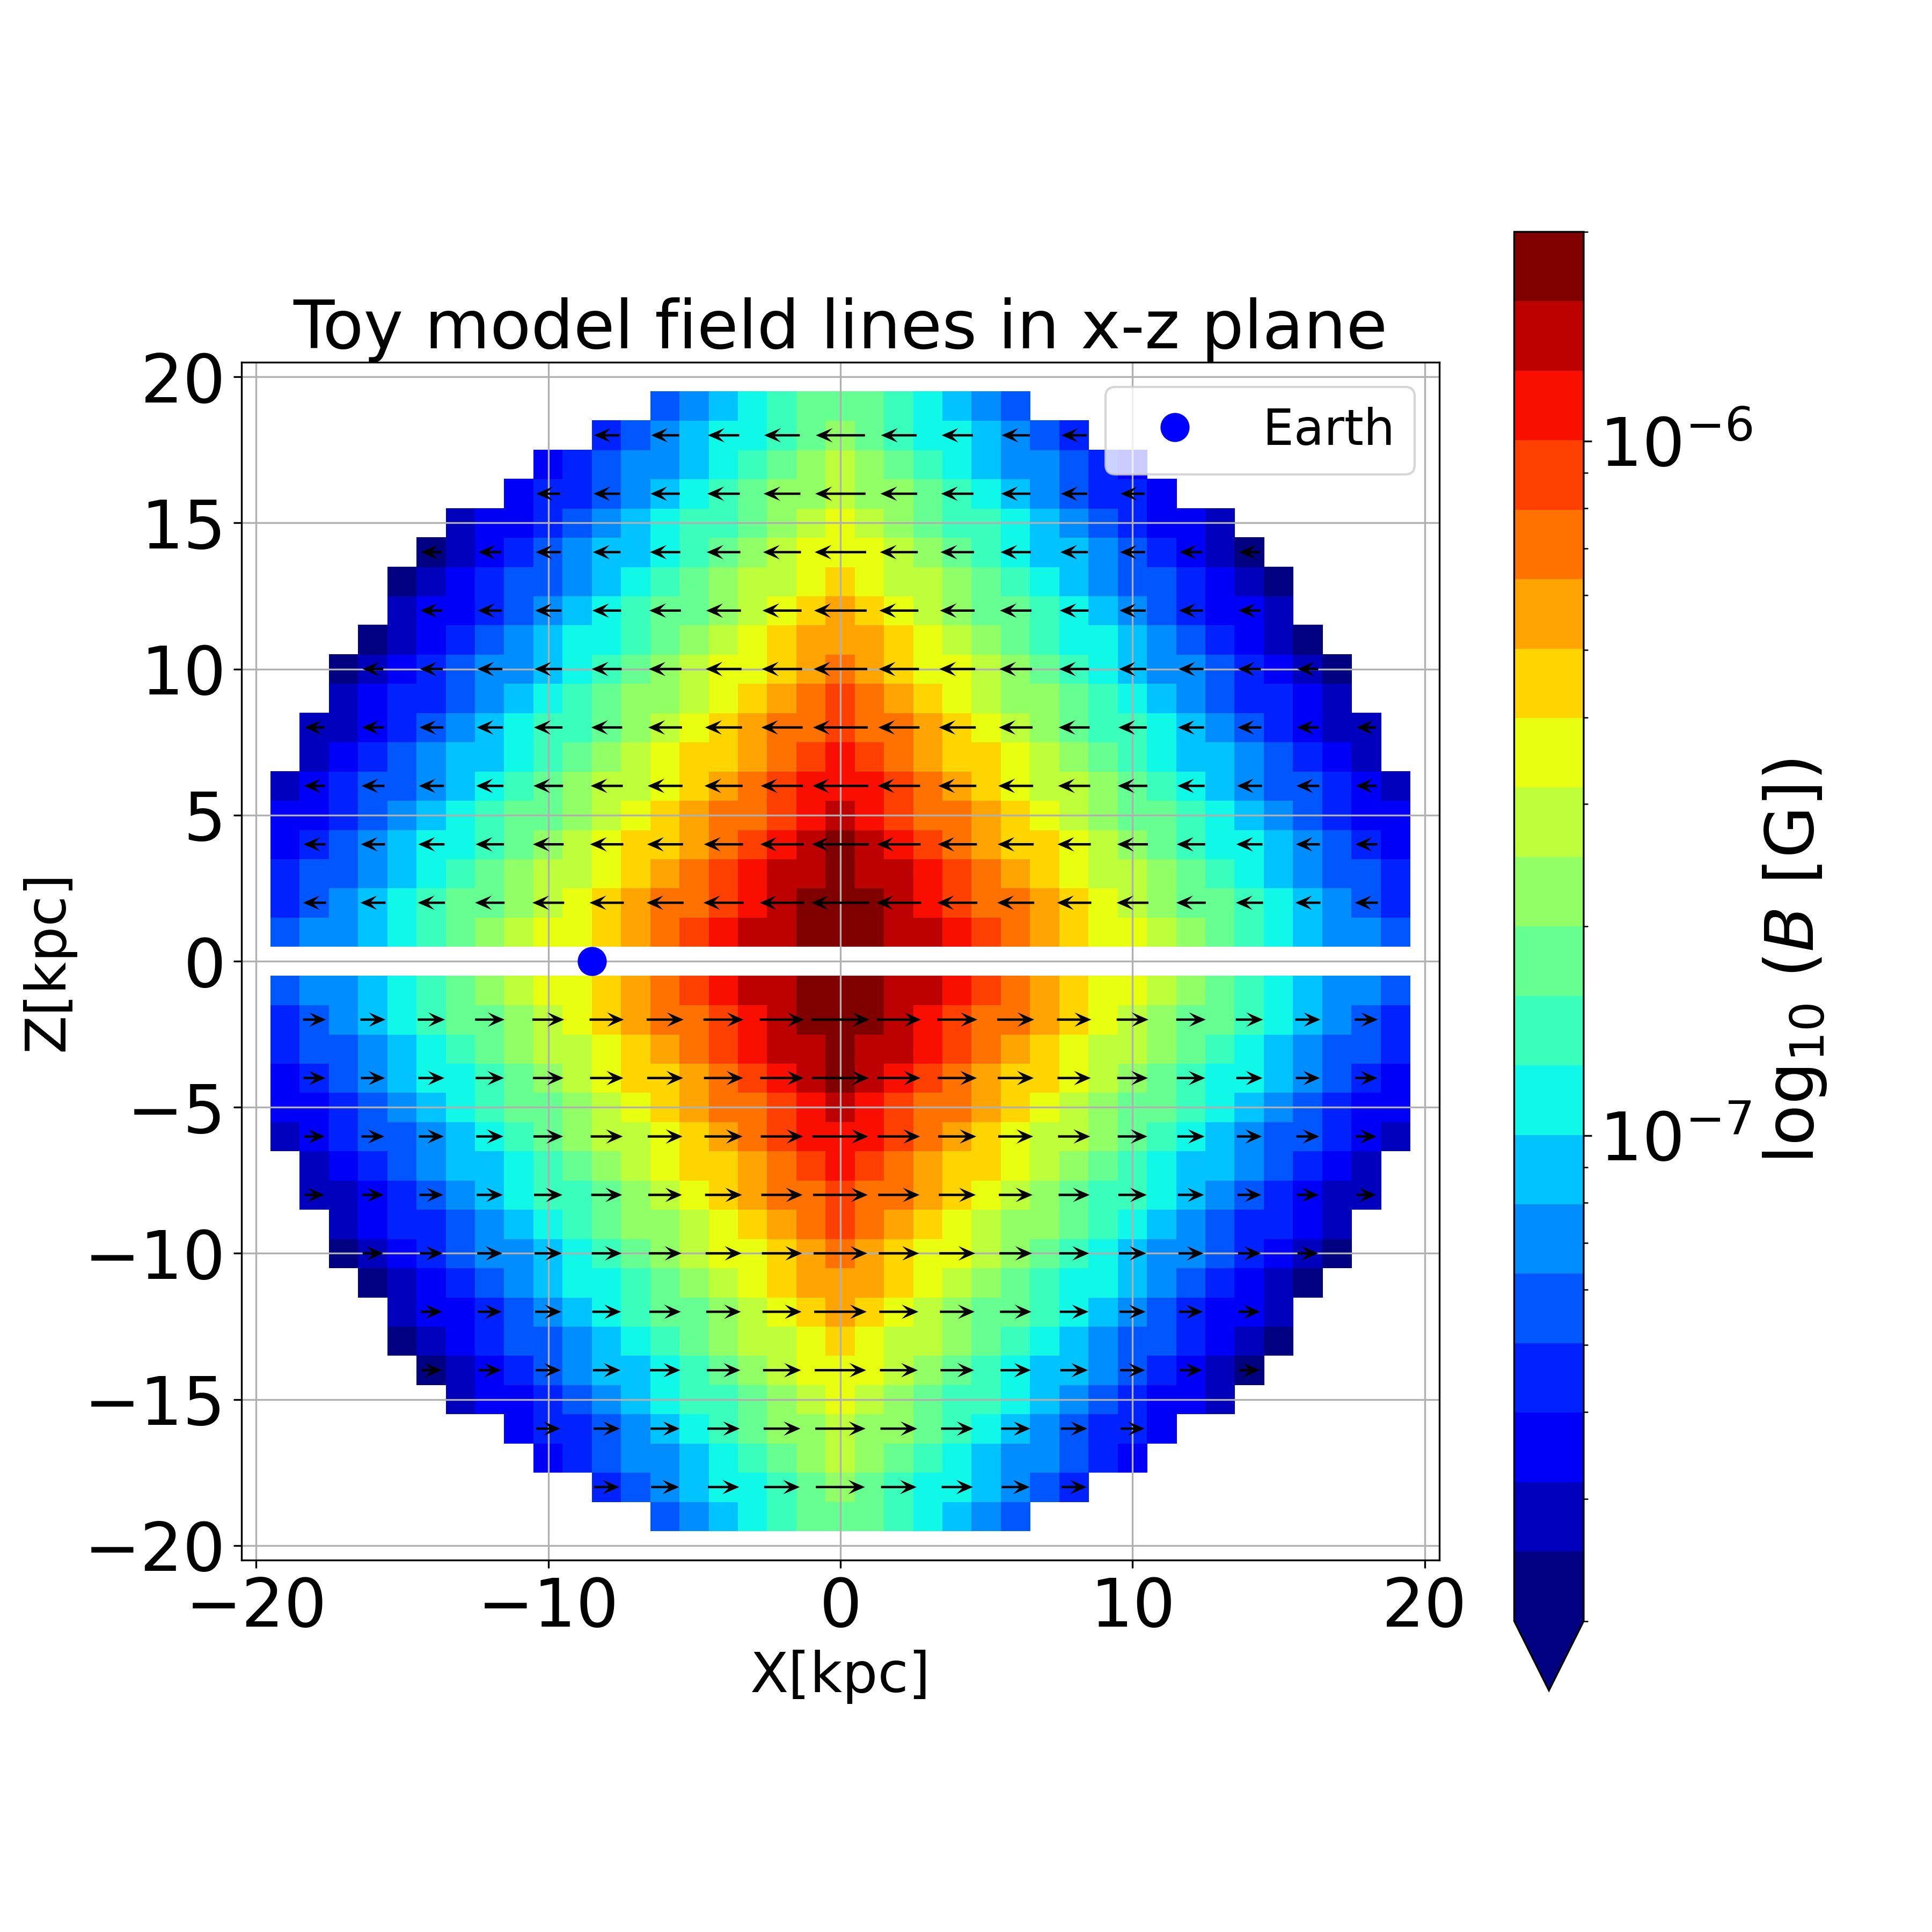
\includegraphics[width = 9cm]{Images/ToyModel_BestFit_XZ.png}%
    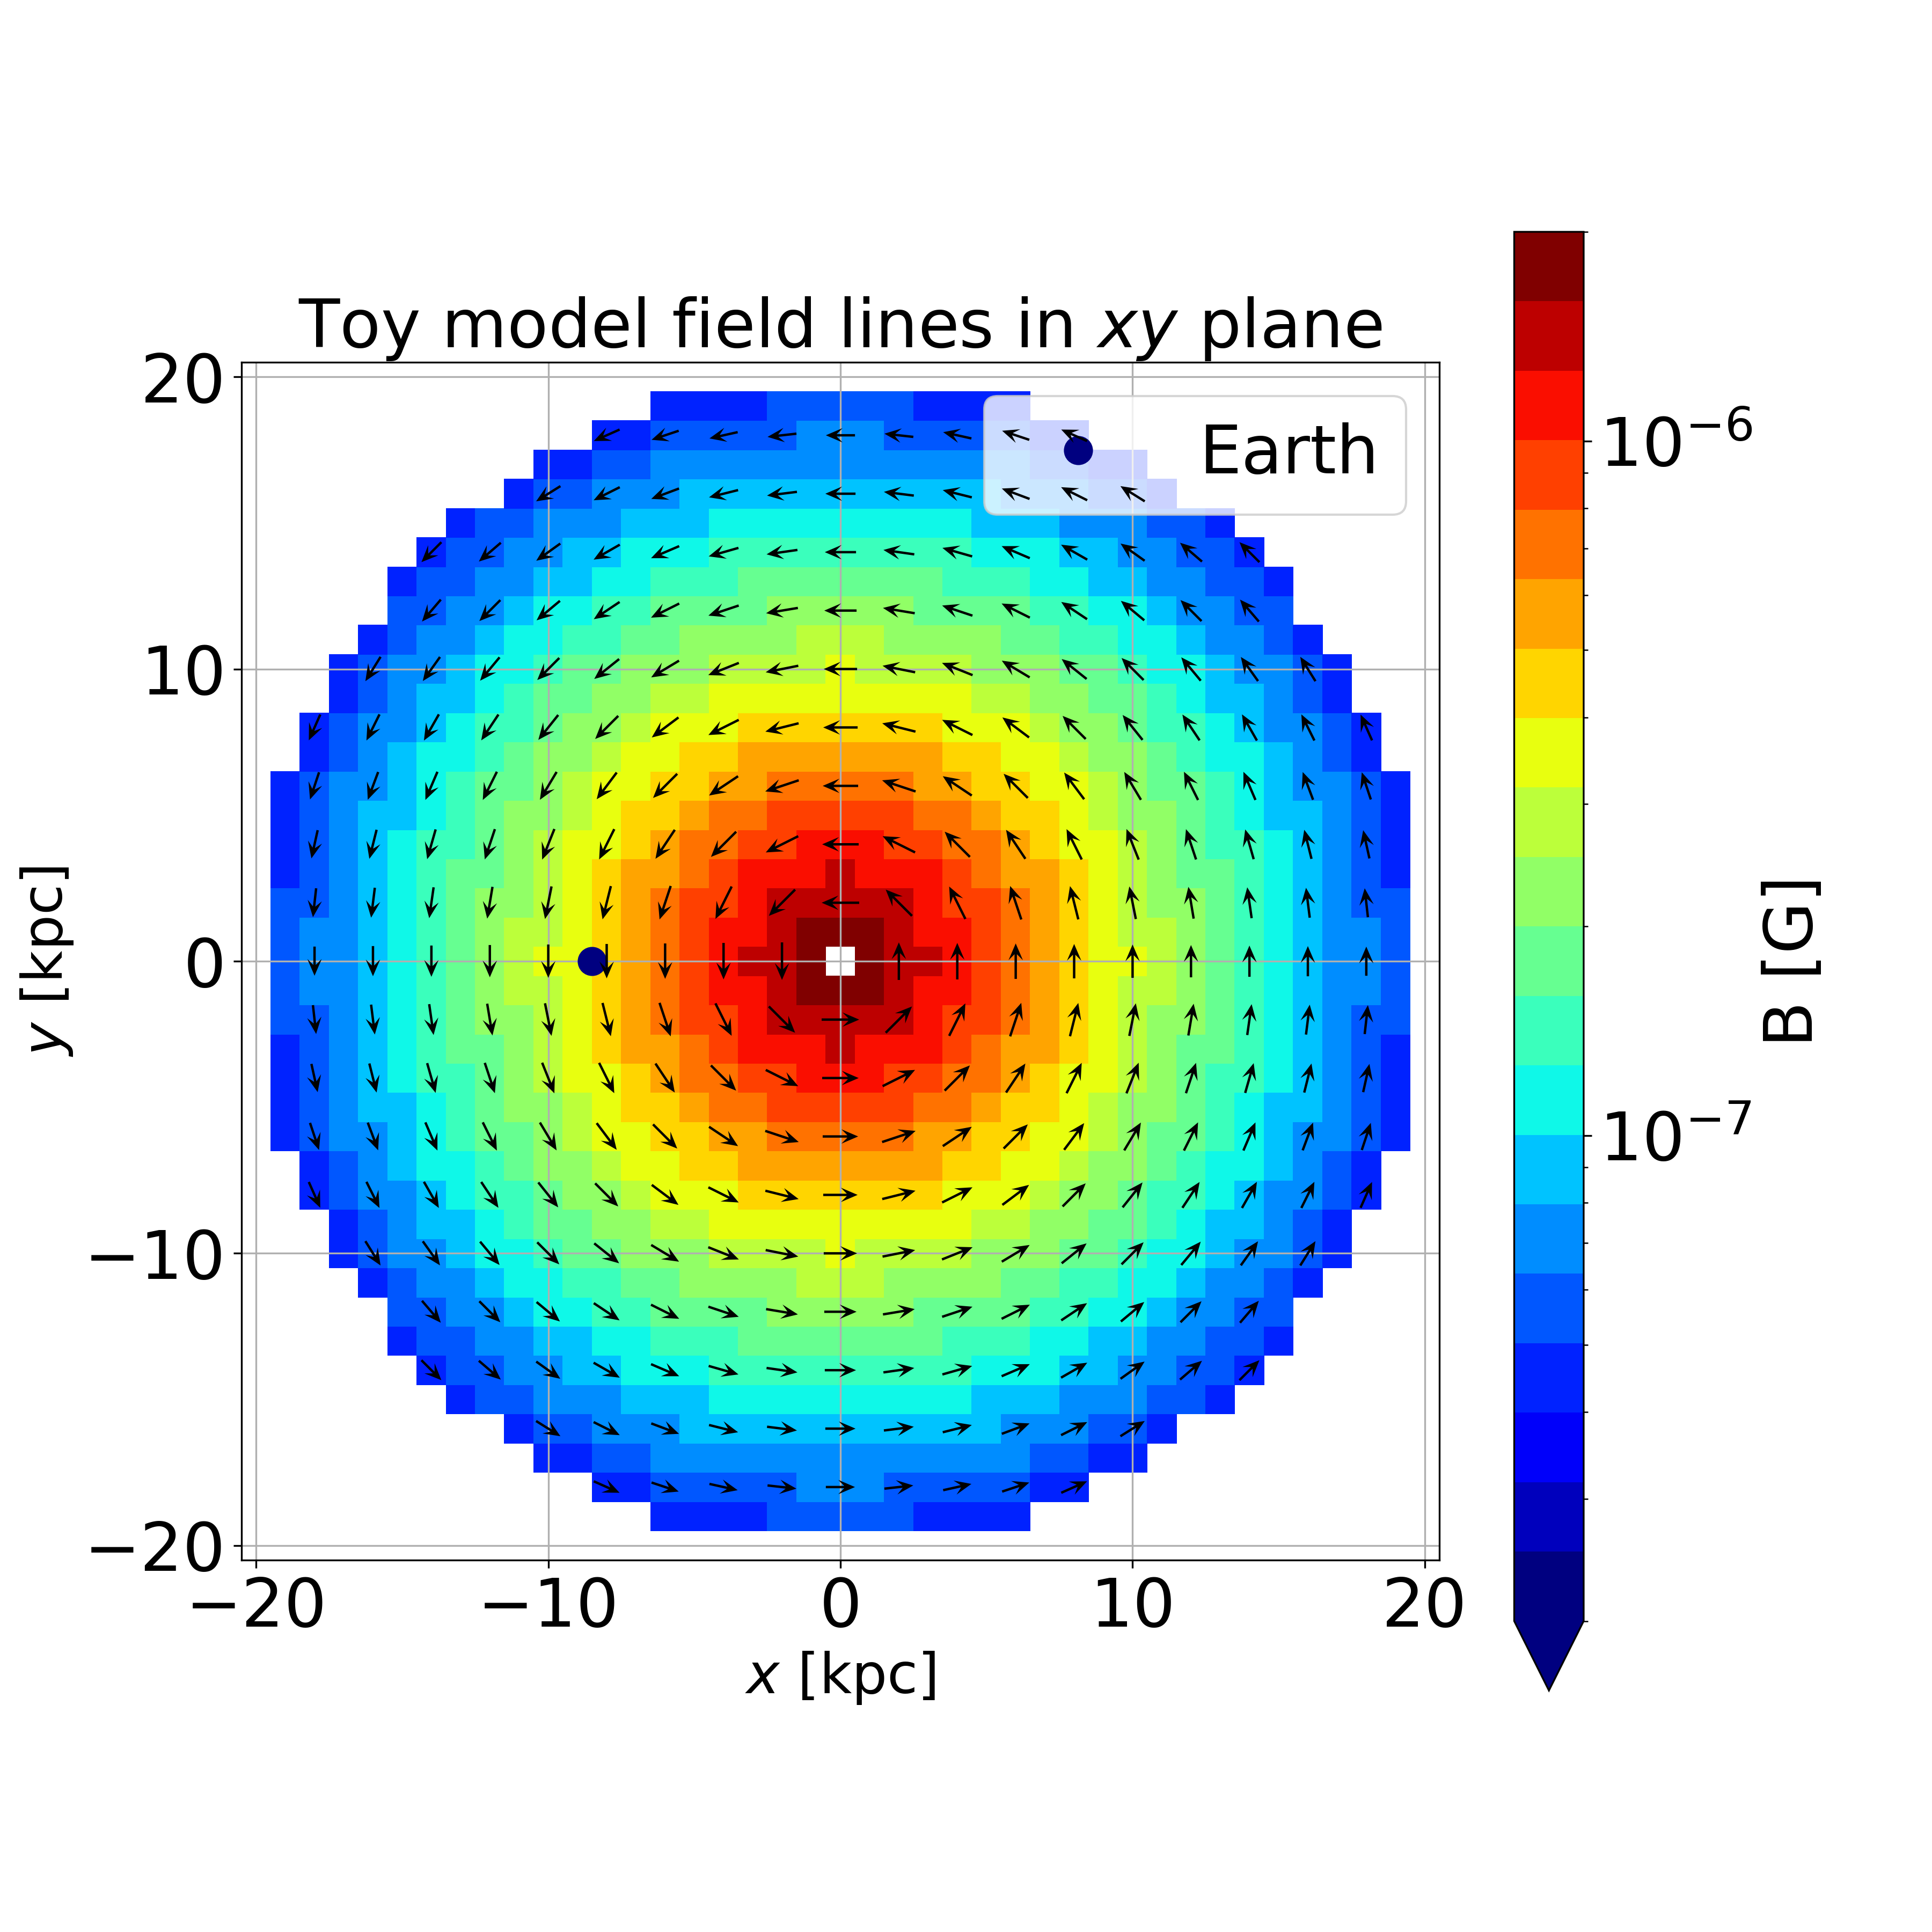
\includegraphics[width = 9cm
    ]{Images/ToyModel_BestFit_XY.png}
    \caption{Cross-section of toy model for the Galactic magnetic field in the Galactic halo region in the XY and XZ plane (with the Galactic plane in the XY plane at $z=0$) showing their drop in two dimensions. \Andrew{REMOVE MOD SIGNS AND VEC NOTATION ON B IN COLAR BAR LABEL}}
    \label{fig:Vis_TM}
\end{figure*}

%Discuss the electron distribution
\subsubsection{Electron Distribution}

In order to produce synthetic synchrotron maps an electron distribution is required.
The JF12 model considered both the WMAP analytical expression \ref{Eq_WMAP_EdNdE}
and simulated electron distribution from GALPROP. They used the latter for their model in their paper.
The two models are quite different. The WMAP \cite{WMAP_Page} model is an analytical expression whereas the GALPROP \cite{Hammurabi} is based on numerical simulations and the distribution of supernova remnants in the Galaxy. For our toy model we adopted the WMAP distribution model. Our current knowledge of the non-thermal electron distribution in the Galaxy, especially in the Galactic halo region, is very limited. We therefore prefer to adopt a simple analytical model in order to avoid adding further layers of complexity. The WMAP electron distribution model is:
\begin{equation}\label{Eq_WMAP_EdNdE}
    \frac{\mathrm{d}N_e}{\mathrm{dlog}E_{e}} =     C_\mathrm{norm} \left(\frac{E_e}{\rm E_{\rm 10 GeV}}\right)^{-p+1} e^{-r/R_{\mathrm{el}}} \mathrm{sech}^2(z/Z_{\mathrm{el}}) 
\end{equation}
where $\frac{\mathrm{d}N_e}{\mathrm{dlog}E_{e}}$ is the differential electron density in a certain energy bins
in units of ${\rm cm}^{-3}$, $p =3$ is the spectral index. The parameters, $C_\mathrm{norm}$, describes the 10~GeV electron density, and $R_{\mathrm{el}}$ \& $Z_{\mathrm{el}}$ describe the radial and azimuthal spatial cut-offs. 


% EdNdE plots for some arbitrary parameters which will be fixed post equipartition scans.
\begin{figure*}
    \centering
    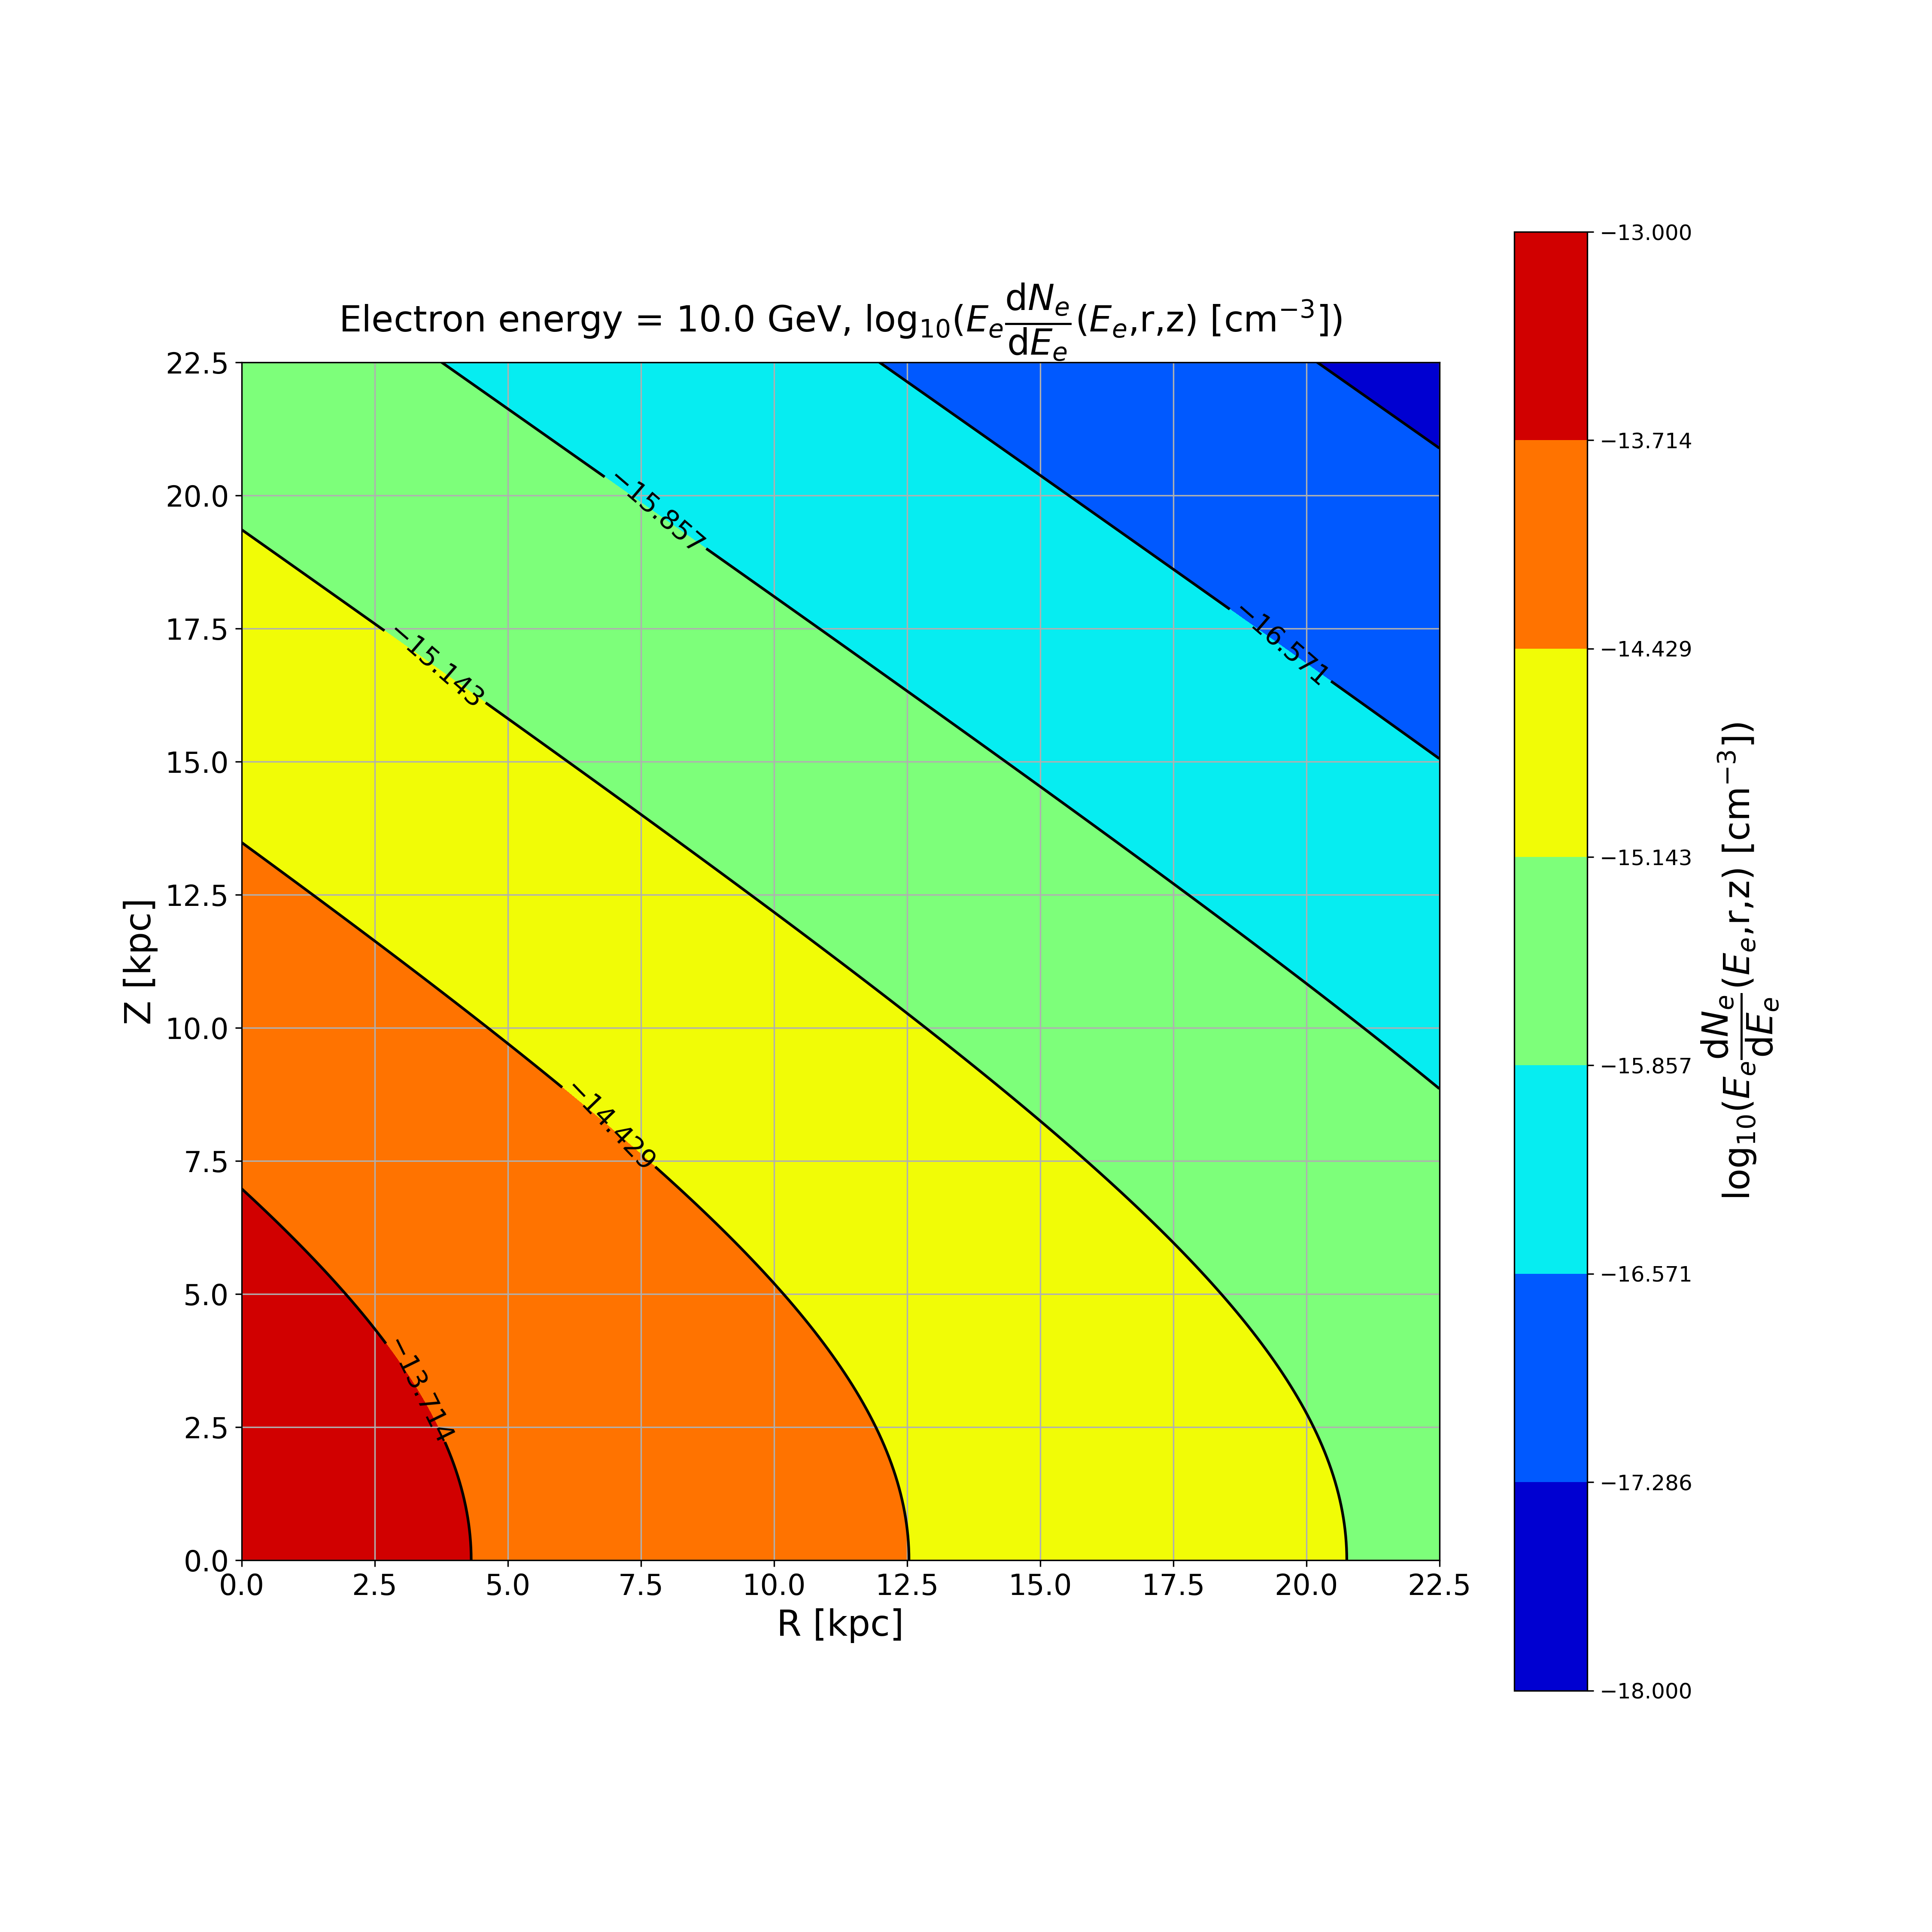
\includegraphics[width= 8cm]{Images/Linear_EdNdE.png}%
    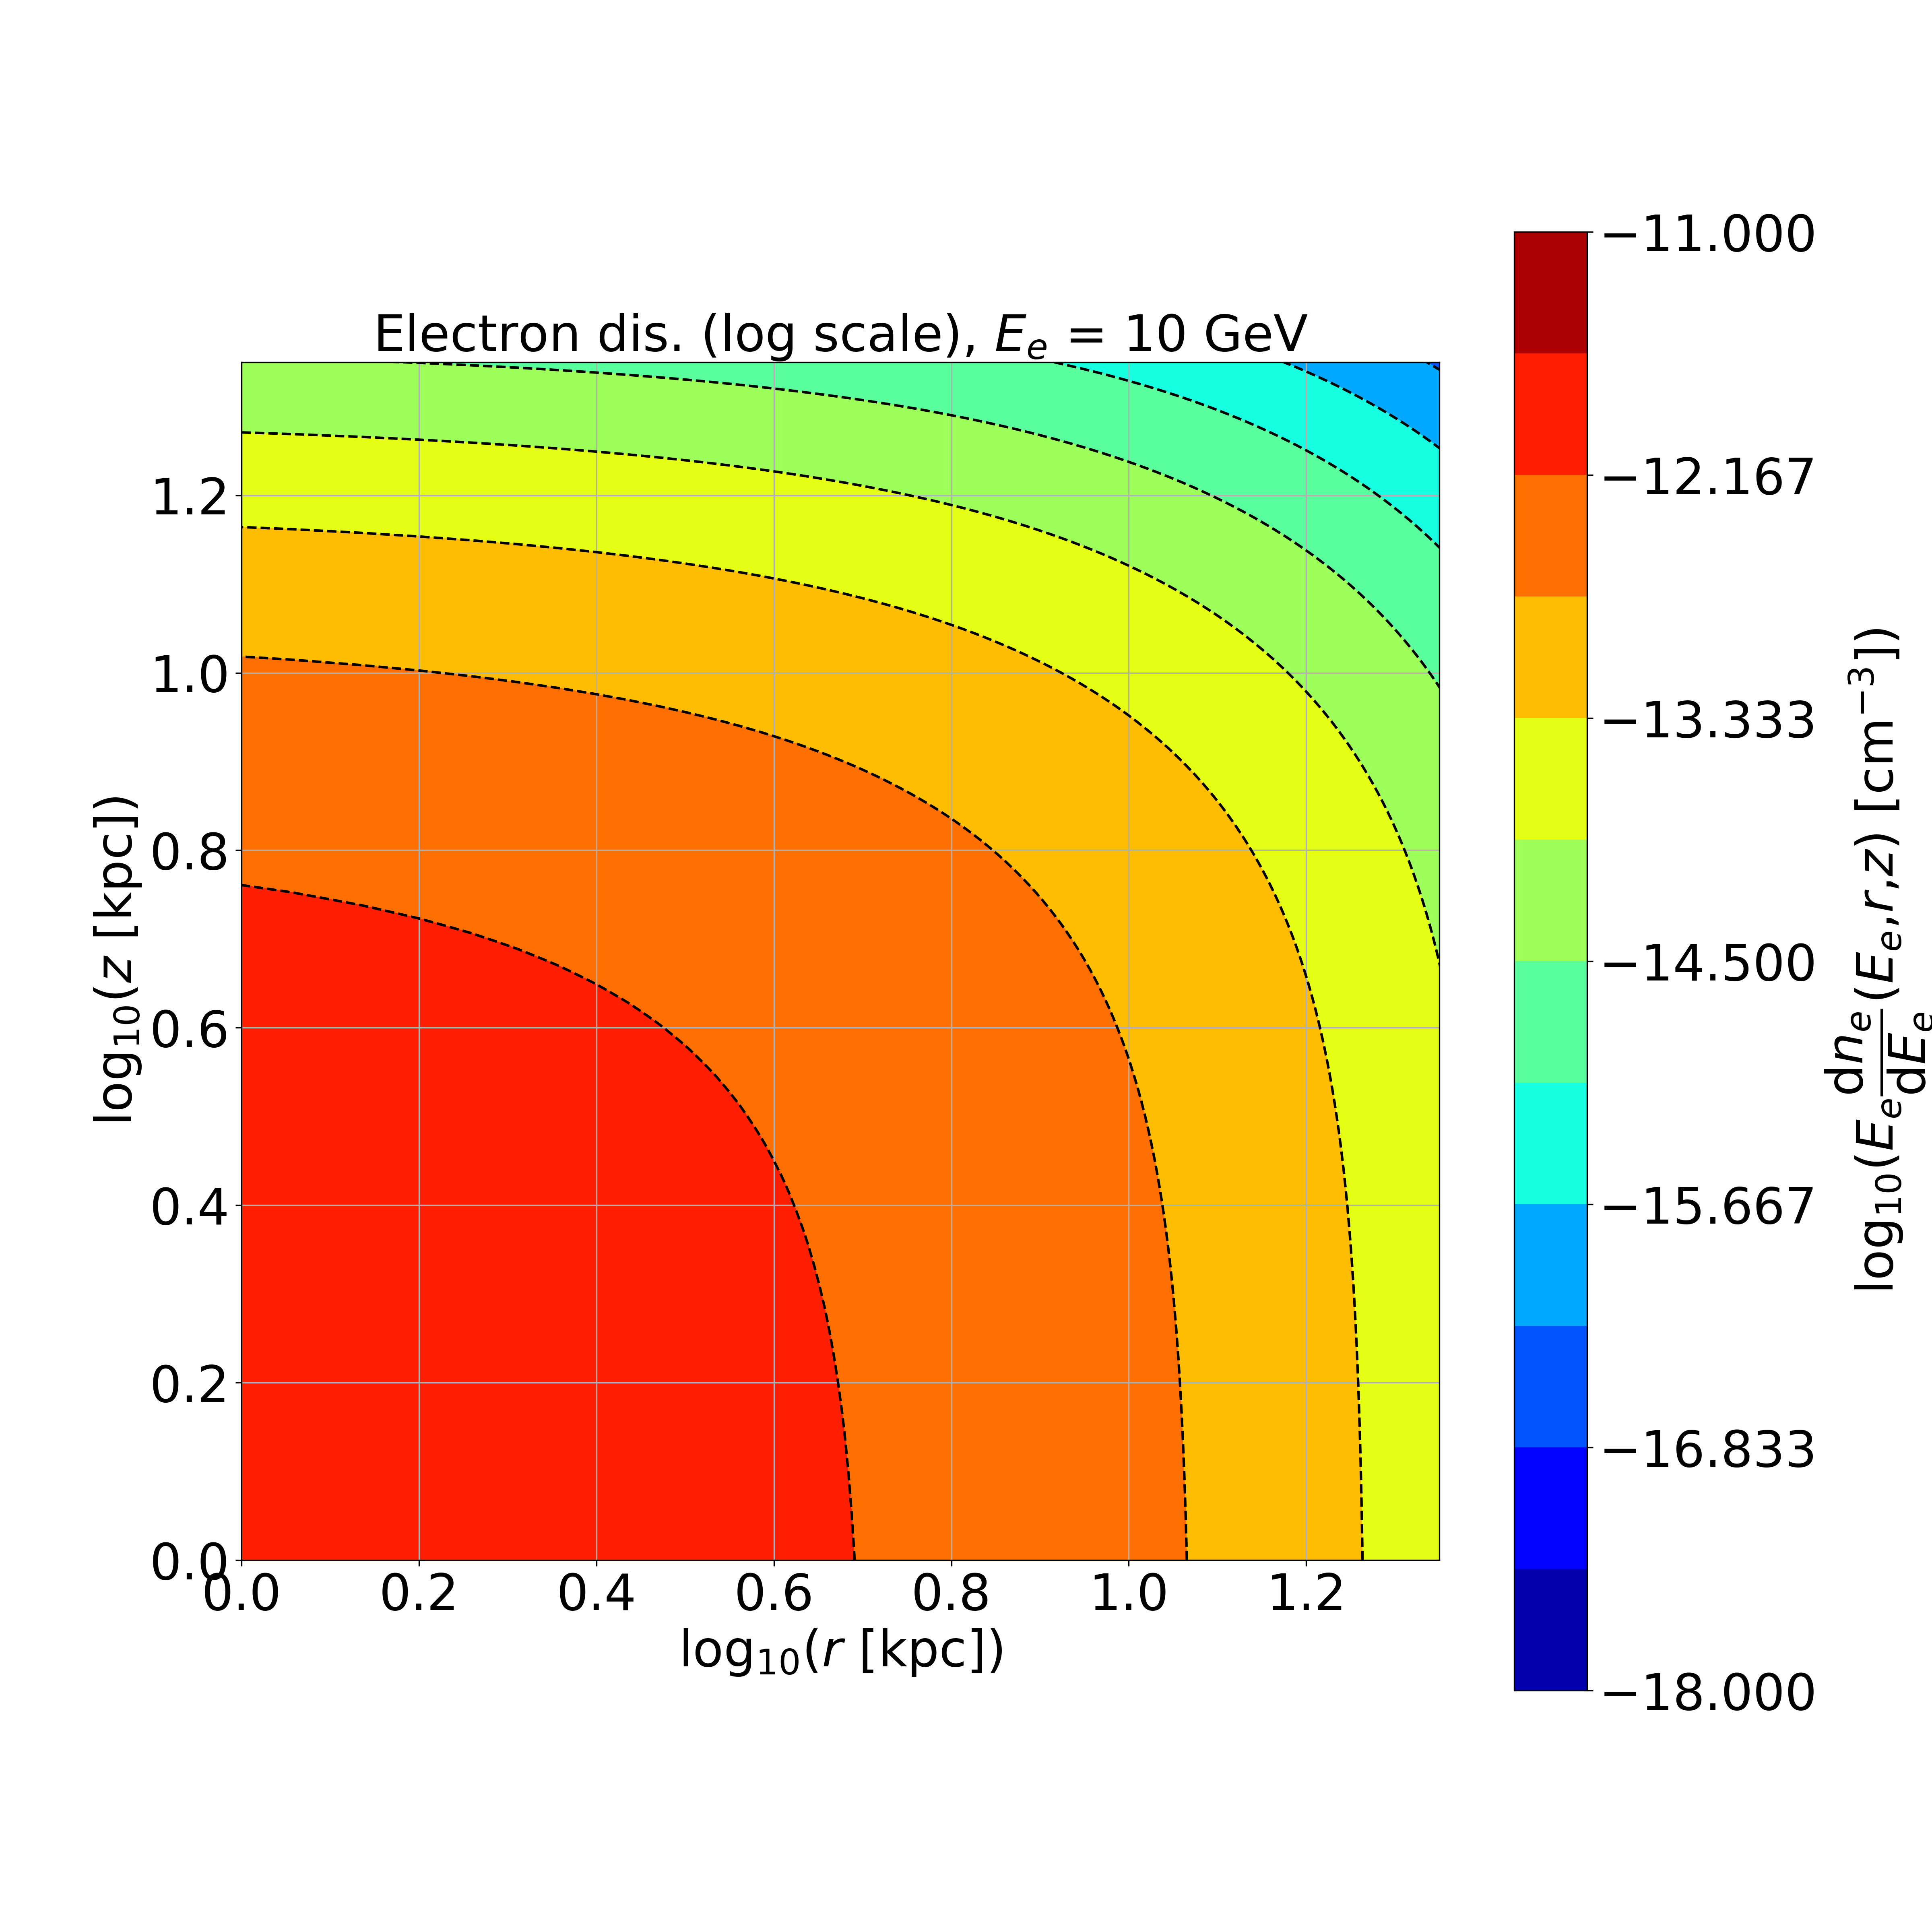
\includegraphics[width = 8cm]{Images/Log_EdNdE.png}
    \caption{Electron distribution for $R_{\mathrm{el}} = 5$ kpc and $Z_{\mathrm{el}} = 7$~kpc in linear scale on left and log-scale on right. \Andrew{LABELS ALL TOO SMALL}}
    \label{fig:my_label}
\end{figure*}

% synchrotron radiation expressions and theory, also the appendix.
\subsection{Synchrotron Emission}\label{Synchrotron_theory}

\subsubsection{Intensity \& polarisation}
Synchrotron radiation or magneto-bremsstrahlung radiation is the radiation produced due to charged particles that gyrate at relativistic speeds around a static magnetic field. The radiation produced via synchrotron is often linearly polarised.

The polarised emission can be visualised as an ellipse where the major axis is the perpendicular component ($J_{\rm \perp}$) and the minor axis is the parallel ($J_{\parallel}$) component. We provide a detailed explanation of this in appendix~(\ref{Appendix_A}). 

The two polarisation emission components, $J_{\perp}$ and $J_{\parallel}$, describe the emission level for a  given peak photon energy $E_{\gamma}^{\mathrm{peak}}$. Expressions for these two components are provided below in eqns~\ref{Jperp} and \ref{Jpara},

\begin{strip}
\begin{equation}
 {J_{\perp}^l} =   \int_{\mathrm{log}E_e^{\mathrm{min}}}^{\mathrm{log}E_e^{\mathrm{max}}}\mathrm{dlog}E_{e} \  \frac{\mathrm{d}N_e}{\mathrm{dlog}E_{e}} \  \left[F\left(\frac{E_{\gamma}}{E_{\gamma}^{\mathrm{peak}}}\right) + G\left(\frac{E_{\gamma}}{E_{\gamma}^{\mathrm{peak}}}\right)\right] * \frac{B_{\perp}}{B_{\mathrm{crit}}}\frac{m_{e}}{h} \frac{8\pi \alpha}{9} 
 \label{Jperp}
\end{equation}
\end{strip}

and,

\begin{strip}
%\begin{widetext}
\begin{equation}
{J_{\parallel}^l} = \int_{\mathrm{log}E_e^{\mathrm{min}}}^{\mathrm{log}E_e^{\mathrm{max}}}\mathrm{dlog}E_{e} \ \frac{\mathrm{d}N_e}{\mathrm{dlog}E_{e}} \  \left[F\left(\frac{E_{\gamma}}{E_{\gamma}^{\mathrm{peak}}}\right) - G\left(\frac{E_{\gamma}}{E_{\gamma}^{\mathrm{peak}}}\right)\right] * \frac{B_{\perp}}{B_{\mathrm{crit}}}\frac{m_{e}}{h} \frac{8\pi \alpha}{9}
\label{Jpara}
\end{equation}
%\end{widetext}
\end{strip}
%\hline

where the functions,
\begin{align}
F(x) &= x \int_x^\infty K_{5/3}(x') dx'\\
G(x) &= x K_{2/3}.
\end{align}
These expressions are provided in terms of the critical field magnetic field strength, $B_{\mathrm{crit}} \frac{m_e^2c^3}{e\hbar} = 4.414 \times 10^{13}$~G, where $m_e = 0.511$~MeV is the mass of electron, $h = 4.136 \times 10^{-15}$~eV-sec is the Planck's constant and $\alpha \approx \frac{1}{137.04}$ is the electromagnetic fine structure constant.

For clarity, several of the conventions we adopted are here noted. The parallel component of polarisation (${J_{\parallel}}$) is orientated in the same direction as  $\vec{B_{\perp}}$, and the perpendicular component of polarisation (${J_{\perp}}$) is perpendicular to $\vec{B_{\perp}}$. The Stokes parameters at each point along the line of sight can be written in terms of the intrinsic polarisation angle $\Psi^l_{\rm in}$ which is the angle between the line of sight perpendicular component of the magnetic field $B_{\perp}$ and Galactic south at each step. The conventions adopted here match those used by the Planck collaboration \cite{Planck_XIX} based on the $\rm HEALPix^3$~\footnote{\textcolor{purple}{https://healpix.jpl.nasa.gov/}} software by \cite{Healpix_2005}. For each step along the line-of-sight, both  ${J_{\perp}^l}$ and ${J_{\parallel}^l}$ are subsequently used to obtain the $Q$ and $U$ Stokes parameters. The integrated values along the line of sight can be defined as  $Q^{\rm tot}_{\rm in}$ and $U^{\rm tot}_{\rm in}$ as:
\begin{eqnarray}
Q_{\rm in}^{\rm tot} = {\int_0^L \mathrm{d}l \ ({J_{\perp}^l} - J_{\parallel}^l) \ {\cos}(2\Psi^l_{\rm in}) } \\
U_{\rm in}^{\rm tot} = {\int_0^L \mathrm{d}l \ ({J_{\perp}^l} - J_{\parallel}^l) \ {\sin}(2\Psi^l_{\rm in})} \,
\end{eqnarray}

The polarised flux ($I_{\rm pol}$) can then be expressed in terms of the intrinsic Stokes parameters which are integrated along the line of sight (${Q_{\rm in}}$ \& ${U_{\rm in}}$) :
\begin{eqnarray} \label{eq_I_pol}
I_{\rm pol} = \sqrt{(Q_{\rm in}^{\rm tot})^2+(U_{\rm in}^{\rm tot})^2} = J_{\perp}^{\rm tot} - J_{\parallel}^{\rm tot} ,\ \rm and
\end{eqnarray}
\begin{equation} \label{eq_I_tot}
    I_{\rm tot} = J_{\perp}^{\rm tot} + J_{\parallel}^{\rm tot} 
\end{equation}
$J_{\perp}^{\rm tot}$ and $J_{\parallel}^{\rm tot}$ are the resultant magnitudes of emissions in perpendicular and parallel directions and can be given by:
\begin{eqnarray}
J_{\perp}^{\rm tot} = (I_{\rm tot} + I_{\rm pol})/2 \\
J_{\parallel}^{\rm tot} = (I_{\rm tot} - I_{\rm pol})/2 
\end{eqnarray}
In appendix(\ref{Appendix_A}) we explain in detail the relation between these equations with two simplified cases.
The intrinsic polarisation angle $\Psi_{\rm in}$ between the Galactic south and the local magnetic field component perpendicular to the line of sight can be defined as:
\begin{eqnarray}
\tan(2\Psi_{\rm in}) = \frac{U_{\rm in}^{\rm tot}}{Q_{\rm in}^{\rm tot}} 
\end{eqnarray}

%% Details of simulation like scanning range, cuts etc
\subsection{Simulation setup for the polarised synchrotron emission}
%% Grid details
Utilising the setup described in the previous section (see section~\ref{Methods}), we generate a synthetic polarised synchrotron emission map for each parameter set of our toy model. The toy model comprises of 5 free parameters, (see table~\ref{Para_table}). The radial cut-off of the magnetic field and electron distribution is kept identical $R_{\mathrm{Mag}}$ = $R_{\mathrm{el}}$ and the same applies to the azimuthal cut-off $Z_{\mathrm{Mag}}$ = $Z_{\mathrm{el}}$. The reason for this constraint is that synchrotron radiation level depends on both non-thermal electron density and magnetic field strength. Thus, even if the spatial extend of the magnetic field differs from the electron distribution, one can only probe the field in the region where both the field and electrons are present. The minimum and maximum value for the spatial parameters are 2~kpc to 19~kpc, which are scanned over in step size of 1~kpc. The range over which both $B_{\rm str}$ and $B_{\rm tur}$ are scanned is 2$~\mu$G to 19$~\mu$G, with a step size of 1$~\mu$G. We calculate the polarised emission for one particular value of $\log_{10}(C_{\rm norm}[{\rm cm}^{-3}]) = -13.85$, and subsequently re-scale these results to obtain the polarised emission maps for different values of  $\log_{10}(C_{\rm norm} [{\rm cm}^{-3}])$, ranging this scan from $-9.84$ to $-15.83$ with a step size of $0.24$ (ie. in 25 steps).

%% Handling of data 
In our study, we mask out three regions from our skymaps. The first of these is in the Galactic disc region between b = $(-15^{\circ},15^{\circ})$. For the second region, based on observations from \cite{eROSITA} and \cite{Su_2010}, we block out longitudes  $\geq \pm 90^{\circ}$ from the Galactic center (ie. all direction pointing away from the Galactic center direction), so as to ensure that our analysis only covers the region occupied by the Galactic Halo (Fermi and eRosita) bubbles. Lastly, we block out the region associated with the North Polar Spur (NPS). Our motivation here is that the higher latitudes of NPS seem to follow a trend to be originating locally rather than from Galactic center based on the starlight polarisation observations \cite{Gina_2021}. In order to remain as impartial as possible for the designation of this region, we adopt a cut for it selected in \cite{Wolleben_2007}. In fig.~\ref{fig:Skymaps} observational and synthetic skymaps are shown with these three regions removed.

%% Skymap comparison and explanation of smoothening method

To obtain best-fit for our model we ran a grid search for over a million configurations. For each toy configuration, a synthetic skymap was generated using Healpix \cite{Healpix_2005}, adopting a resolution with Nside = 32. Since the interests of our study are focused on large scale structures, both the synthetic skymaps and observational data were smoothed out, using a Gaussian kernel, on size scale of $15^{\circ}$, to wash out smaller scale features. We then compare the simulated polarised emission with the Planck data at 30~GHz by evaluating the $\chi^{2}$ value of the model fit to the data. To find the best fit parameters and their constraints, we carry out a grid search over the 5 free parameters, sampling in total two million parameter points.


\subsection{Observational Data}
% discussion of data sets used
For our synchrotron emission study We use the publicly available from the Planck satellite mission \footnote{\textcolor{purple}{http://pla.esac.esa.int/pla/}}. Specifically, we use the polarised radio data at 30~GHz from Planck where the peak frequency is at 28.4~GHz, with a band width of 9.8~GHz. At this frequency a considerable level of polarised synchrotron emission is observed, with a only a small level of Faraday rotation occurring at these high frequencies. However, we also note that in this 30~GHz band, the Planck data cannot be used to probe synchrotron intensity directly, since at this frequency the unpolarised sky receives a considerable contributions from both thermal bremsstrahlung and anomalous microwave emission, as well as synchrotron radiation \cite{Planck_XIX} and \cite{Planck_XLII}. 

\subsection{Constraints on Magnetic Field Model}
\label{Results}
%% Details of uncertainities 
We obtained 1$~\sigma$ constraint on our model shown in table~$\ref{Para_table}$. For the structured magnetic field strength $B_{\rm str}$ we obtain the best fit value of 3~$\mu$G with the upper extreme being 11~$\mu$G
and the lower extreme 1~$\mu$G. Similarly, turbulent magnetic fields $B_{\rm tur}$ the mean value is 6~$\mu$G and upper and lower extreme values are 4~$\mu$G and 12~$\mu$G respectively. For spatial dimensions, we obtain a best fit vale of 7~kpc for the azimuthal extent $Z_{\rm Mag}/Z_{\rm el}$ and uncertainities of $\pm$ 1~kpc. Similarly, for electron densities we obtain a best fit value of $3\times 10^{-13} \rm cm^{-3}$ \Vasu{Will update this!} These values are in agreement with the observations made by FERMI \cite{Su_2010}, S-PASS\cite{Carretti_2013} and eROSITA\cite{eROSITA}. We do not however, obtain an upper extreme value for $R_{\rm Mag}/R_{\rm el}$ only a lower extreme value of 4~kpc with the best fit value being 5~kpc. Again this best fit value is in agreement with the radial extent as obtained by the observations.

In Fig.~\ref{fig:Skymaps} the smoothened skymap obtained from the best fit value of the parameters and the smoothened polarised Planck data is shown along with the residuals. The best-fit values used for the parameters are provided in table~\ref{Para_table}. 
%% Polarisation fraction
We next estimate the polarisation fraction obtained by our best-fit toy-model which is given in figure \ref{fig:Skymaps} which was calculated taking the ratio of the polarised to the total intensity. The polarisation fraction for the best-fit toy model is comparable to the values as seen in the observation data \cite{Carretti_2013} and \cite{WMAP_Page}.

%% Polarised Skymap

\begin{figure*}
\centering
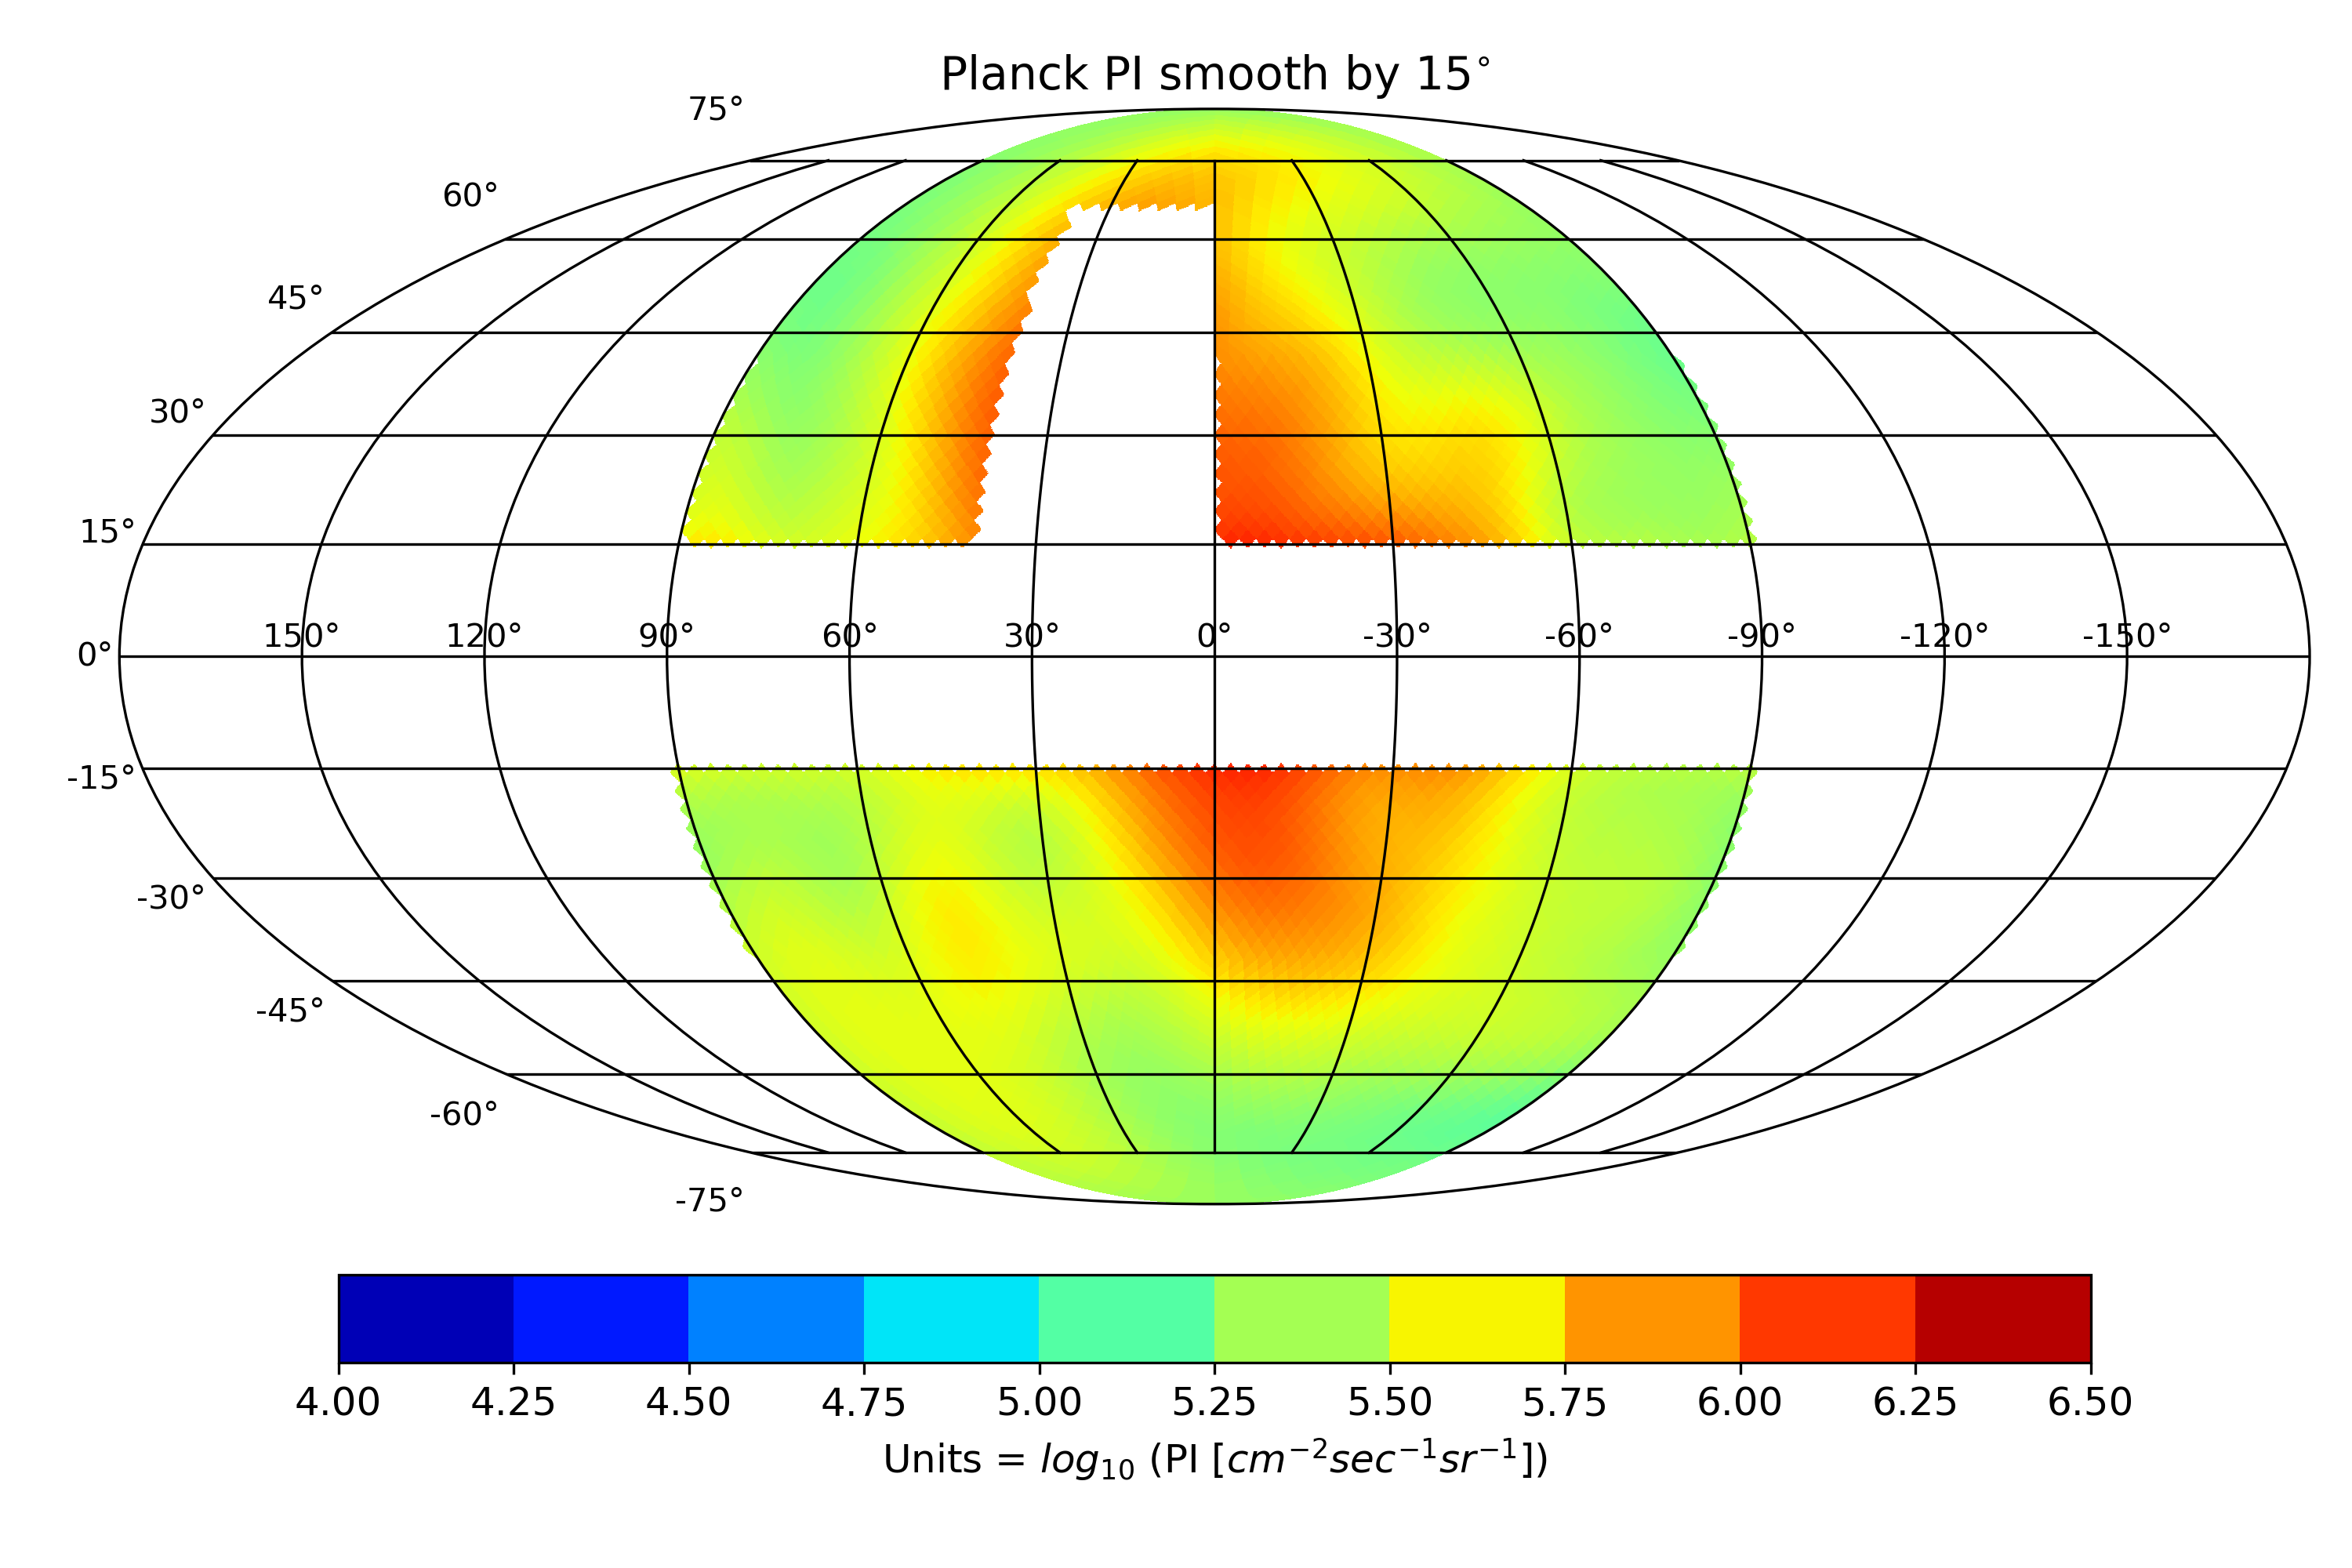
\includegraphics[width =0.49\linewidth]{Images/Jan-17-2022_Planck_Sky_Map.png}%
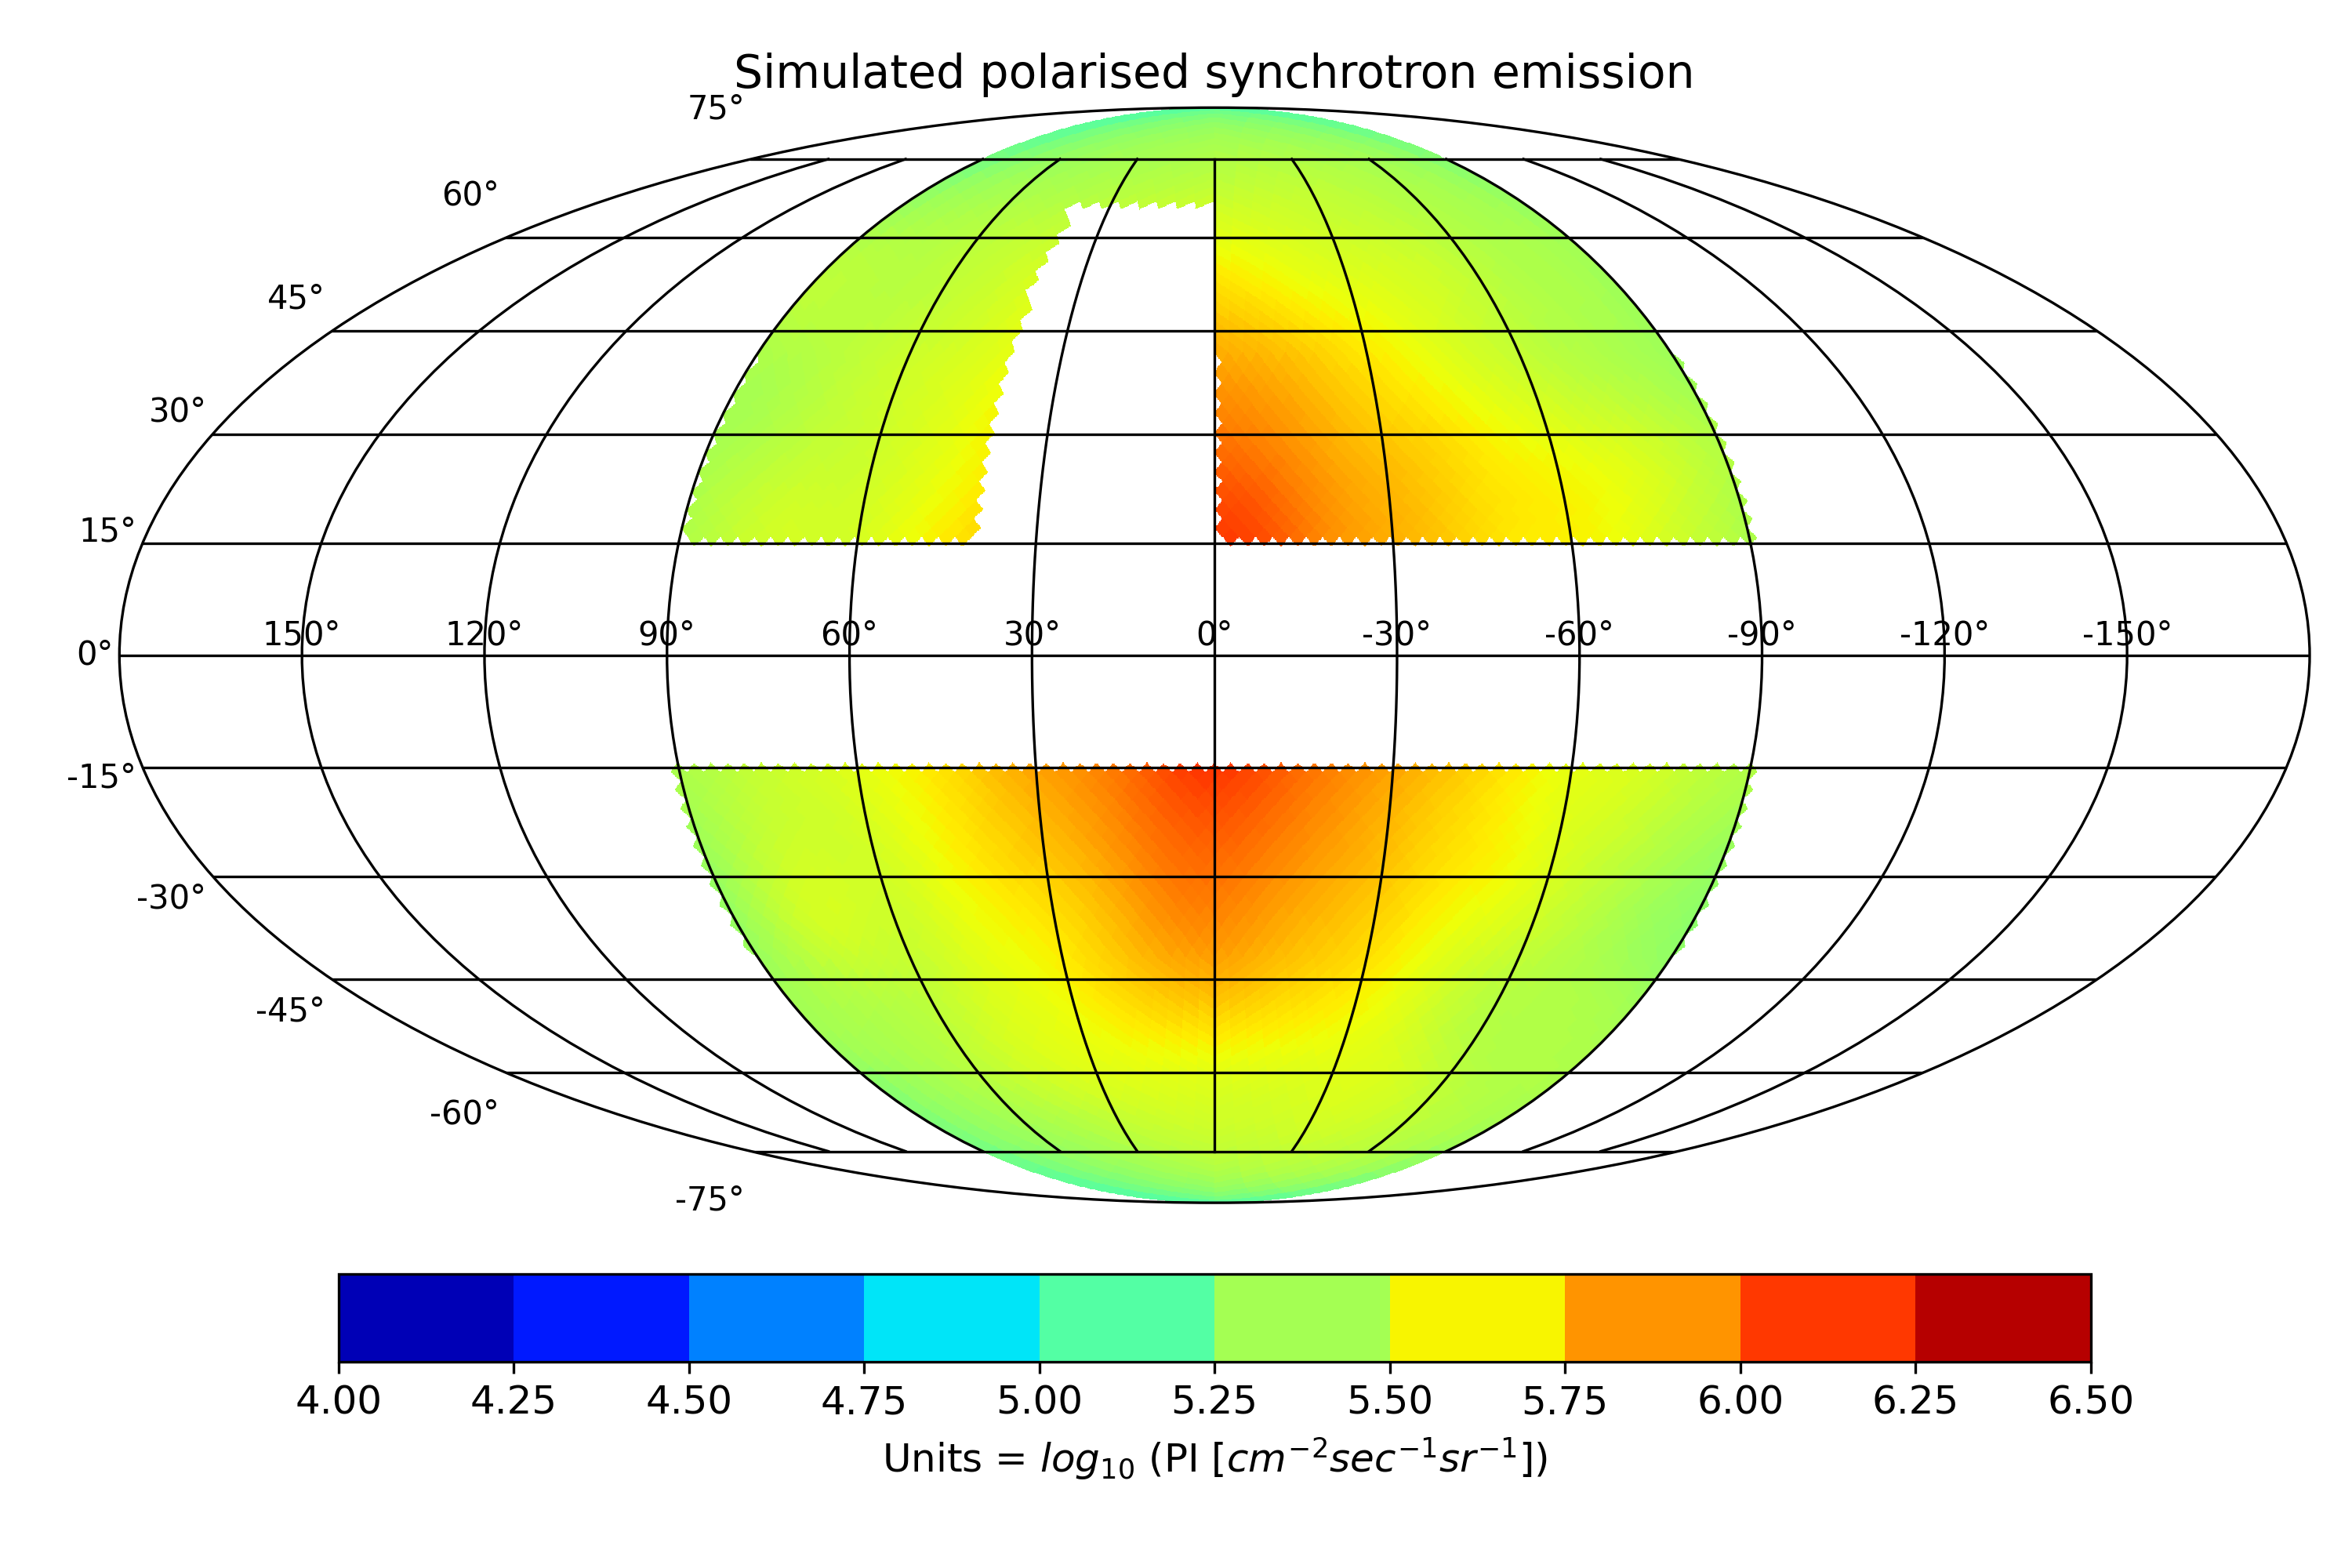
\includegraphics[width=0.49\linewidth]{Images/Jan-20-2022Ver1_Skymap_Bstr_3_Btur_6_Rmag_5_Zmag_7_norm_3.76e-13.png}
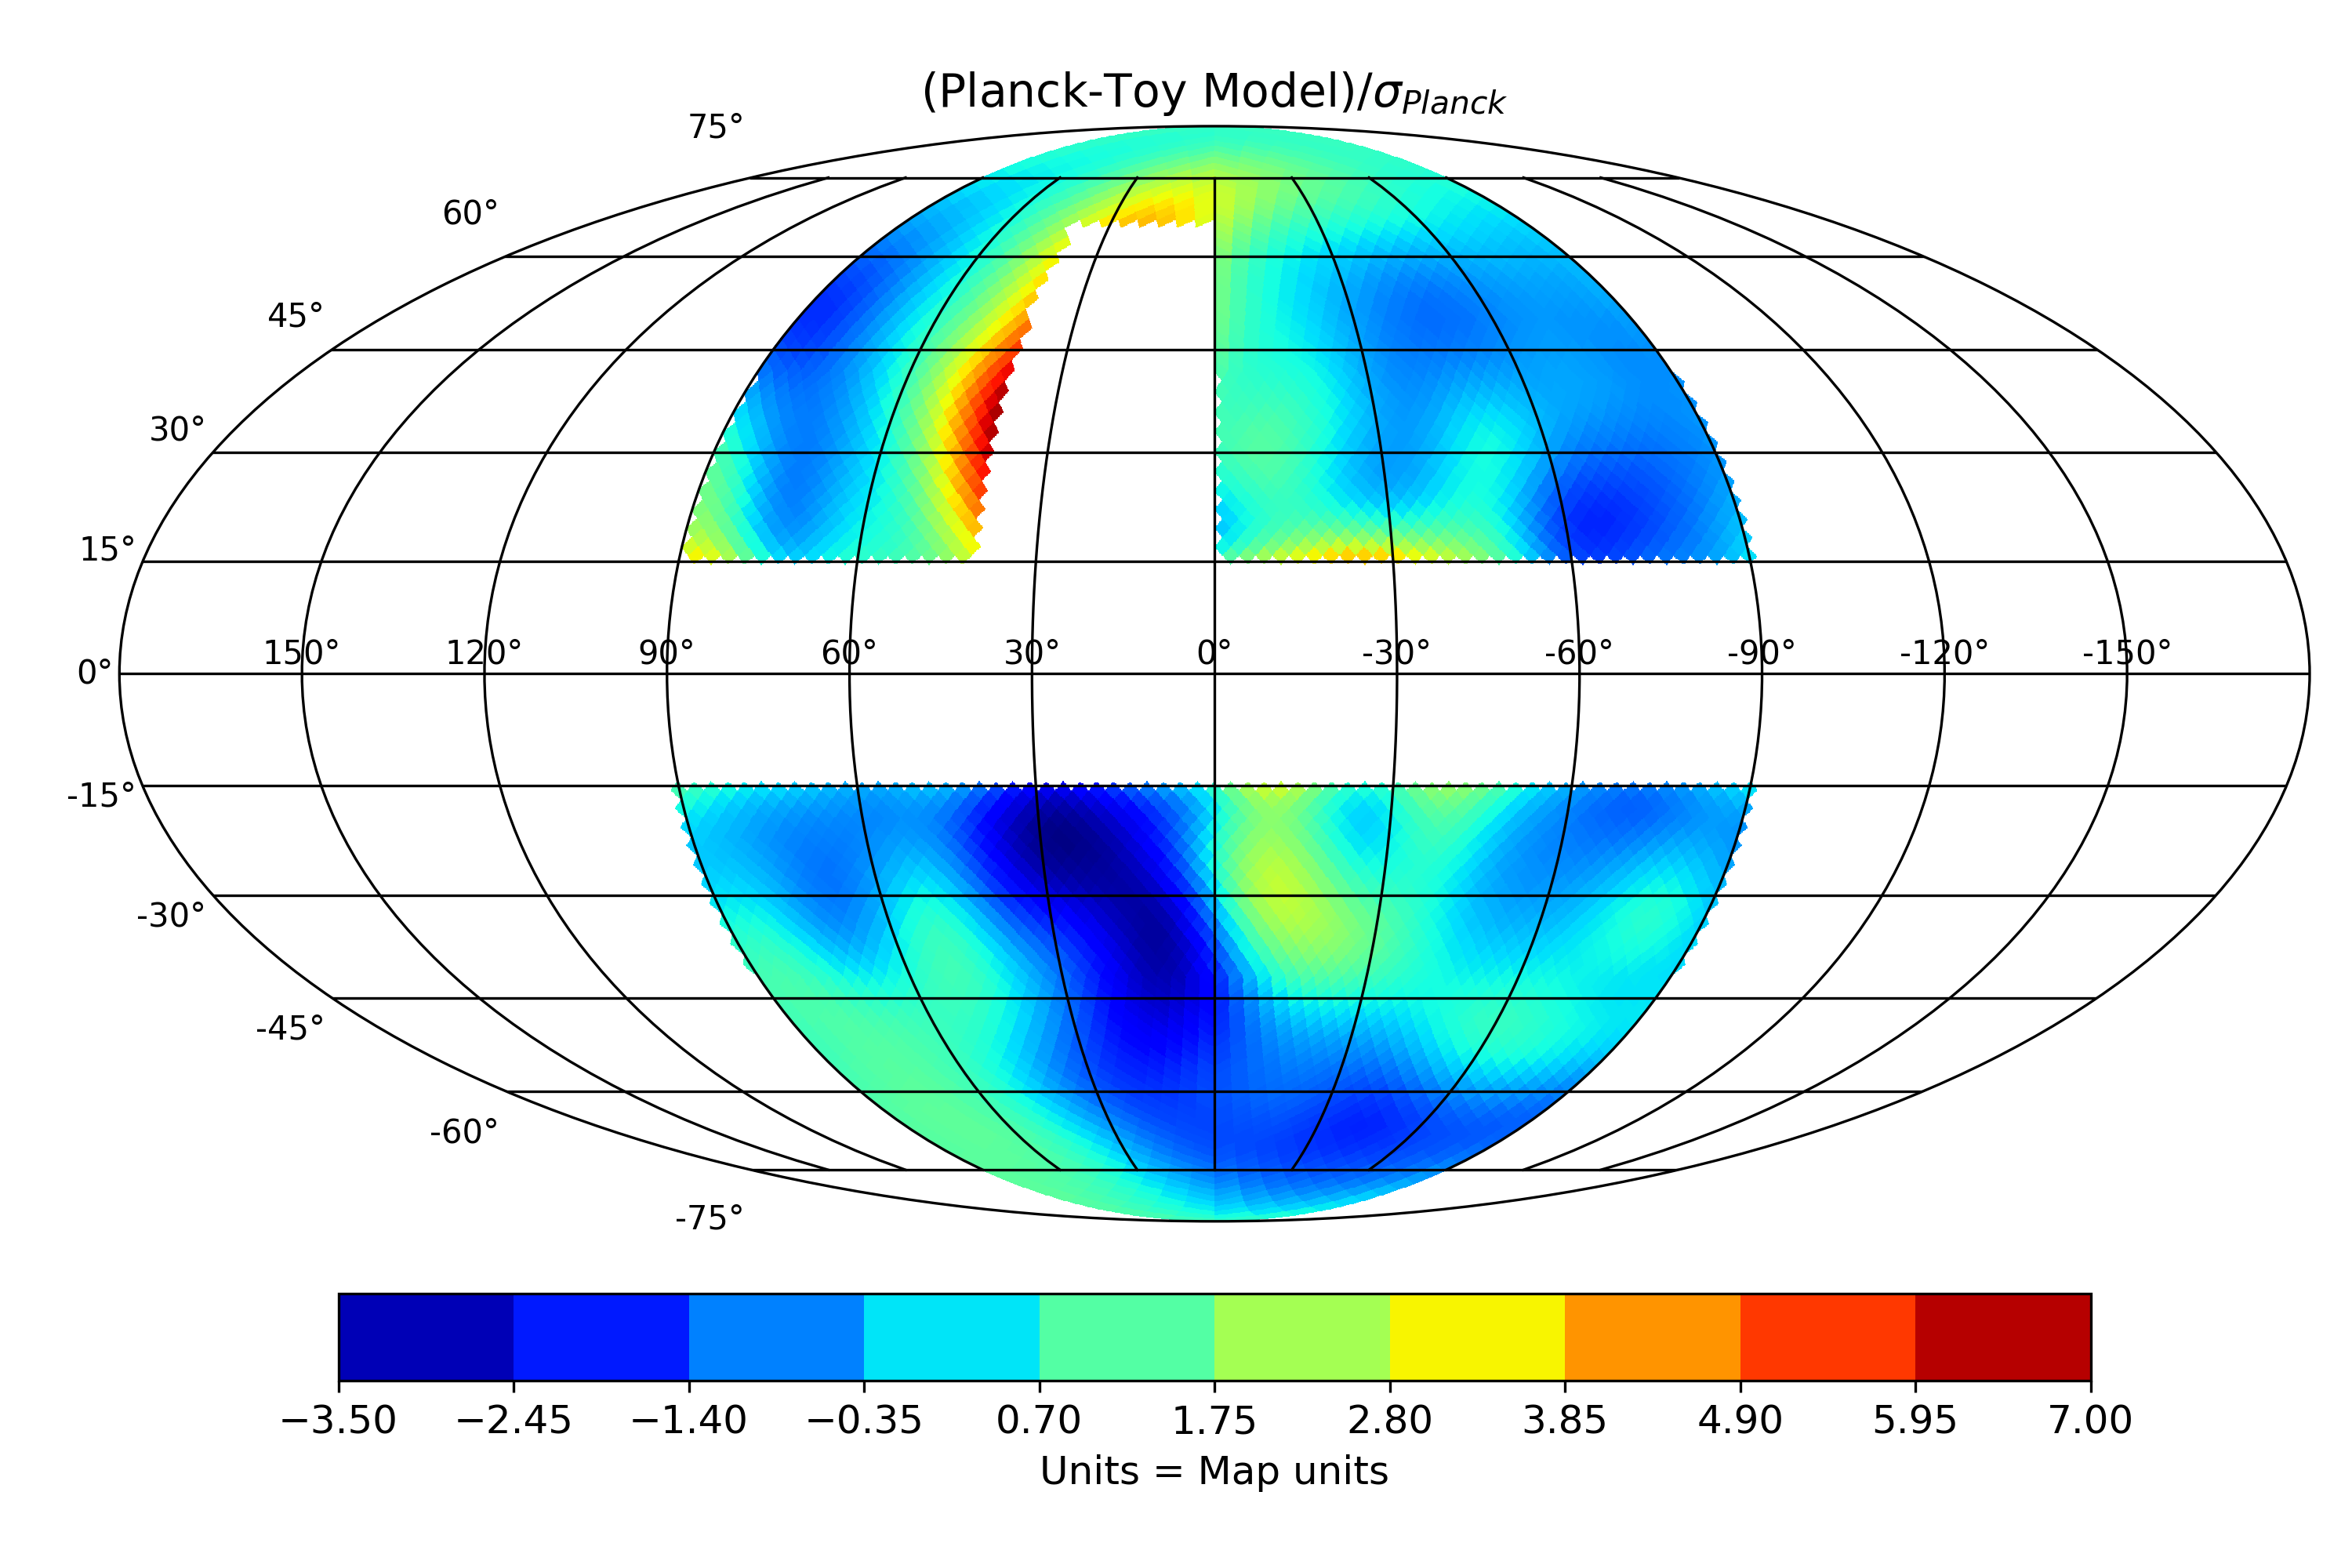
\includegraphics[width = 0.49\linewidth]{Images/Jan-20-2022_Residue_Bstr_3_Btur_6_Rmag_5_Zmag_7_norm_3.76e-13.png}%
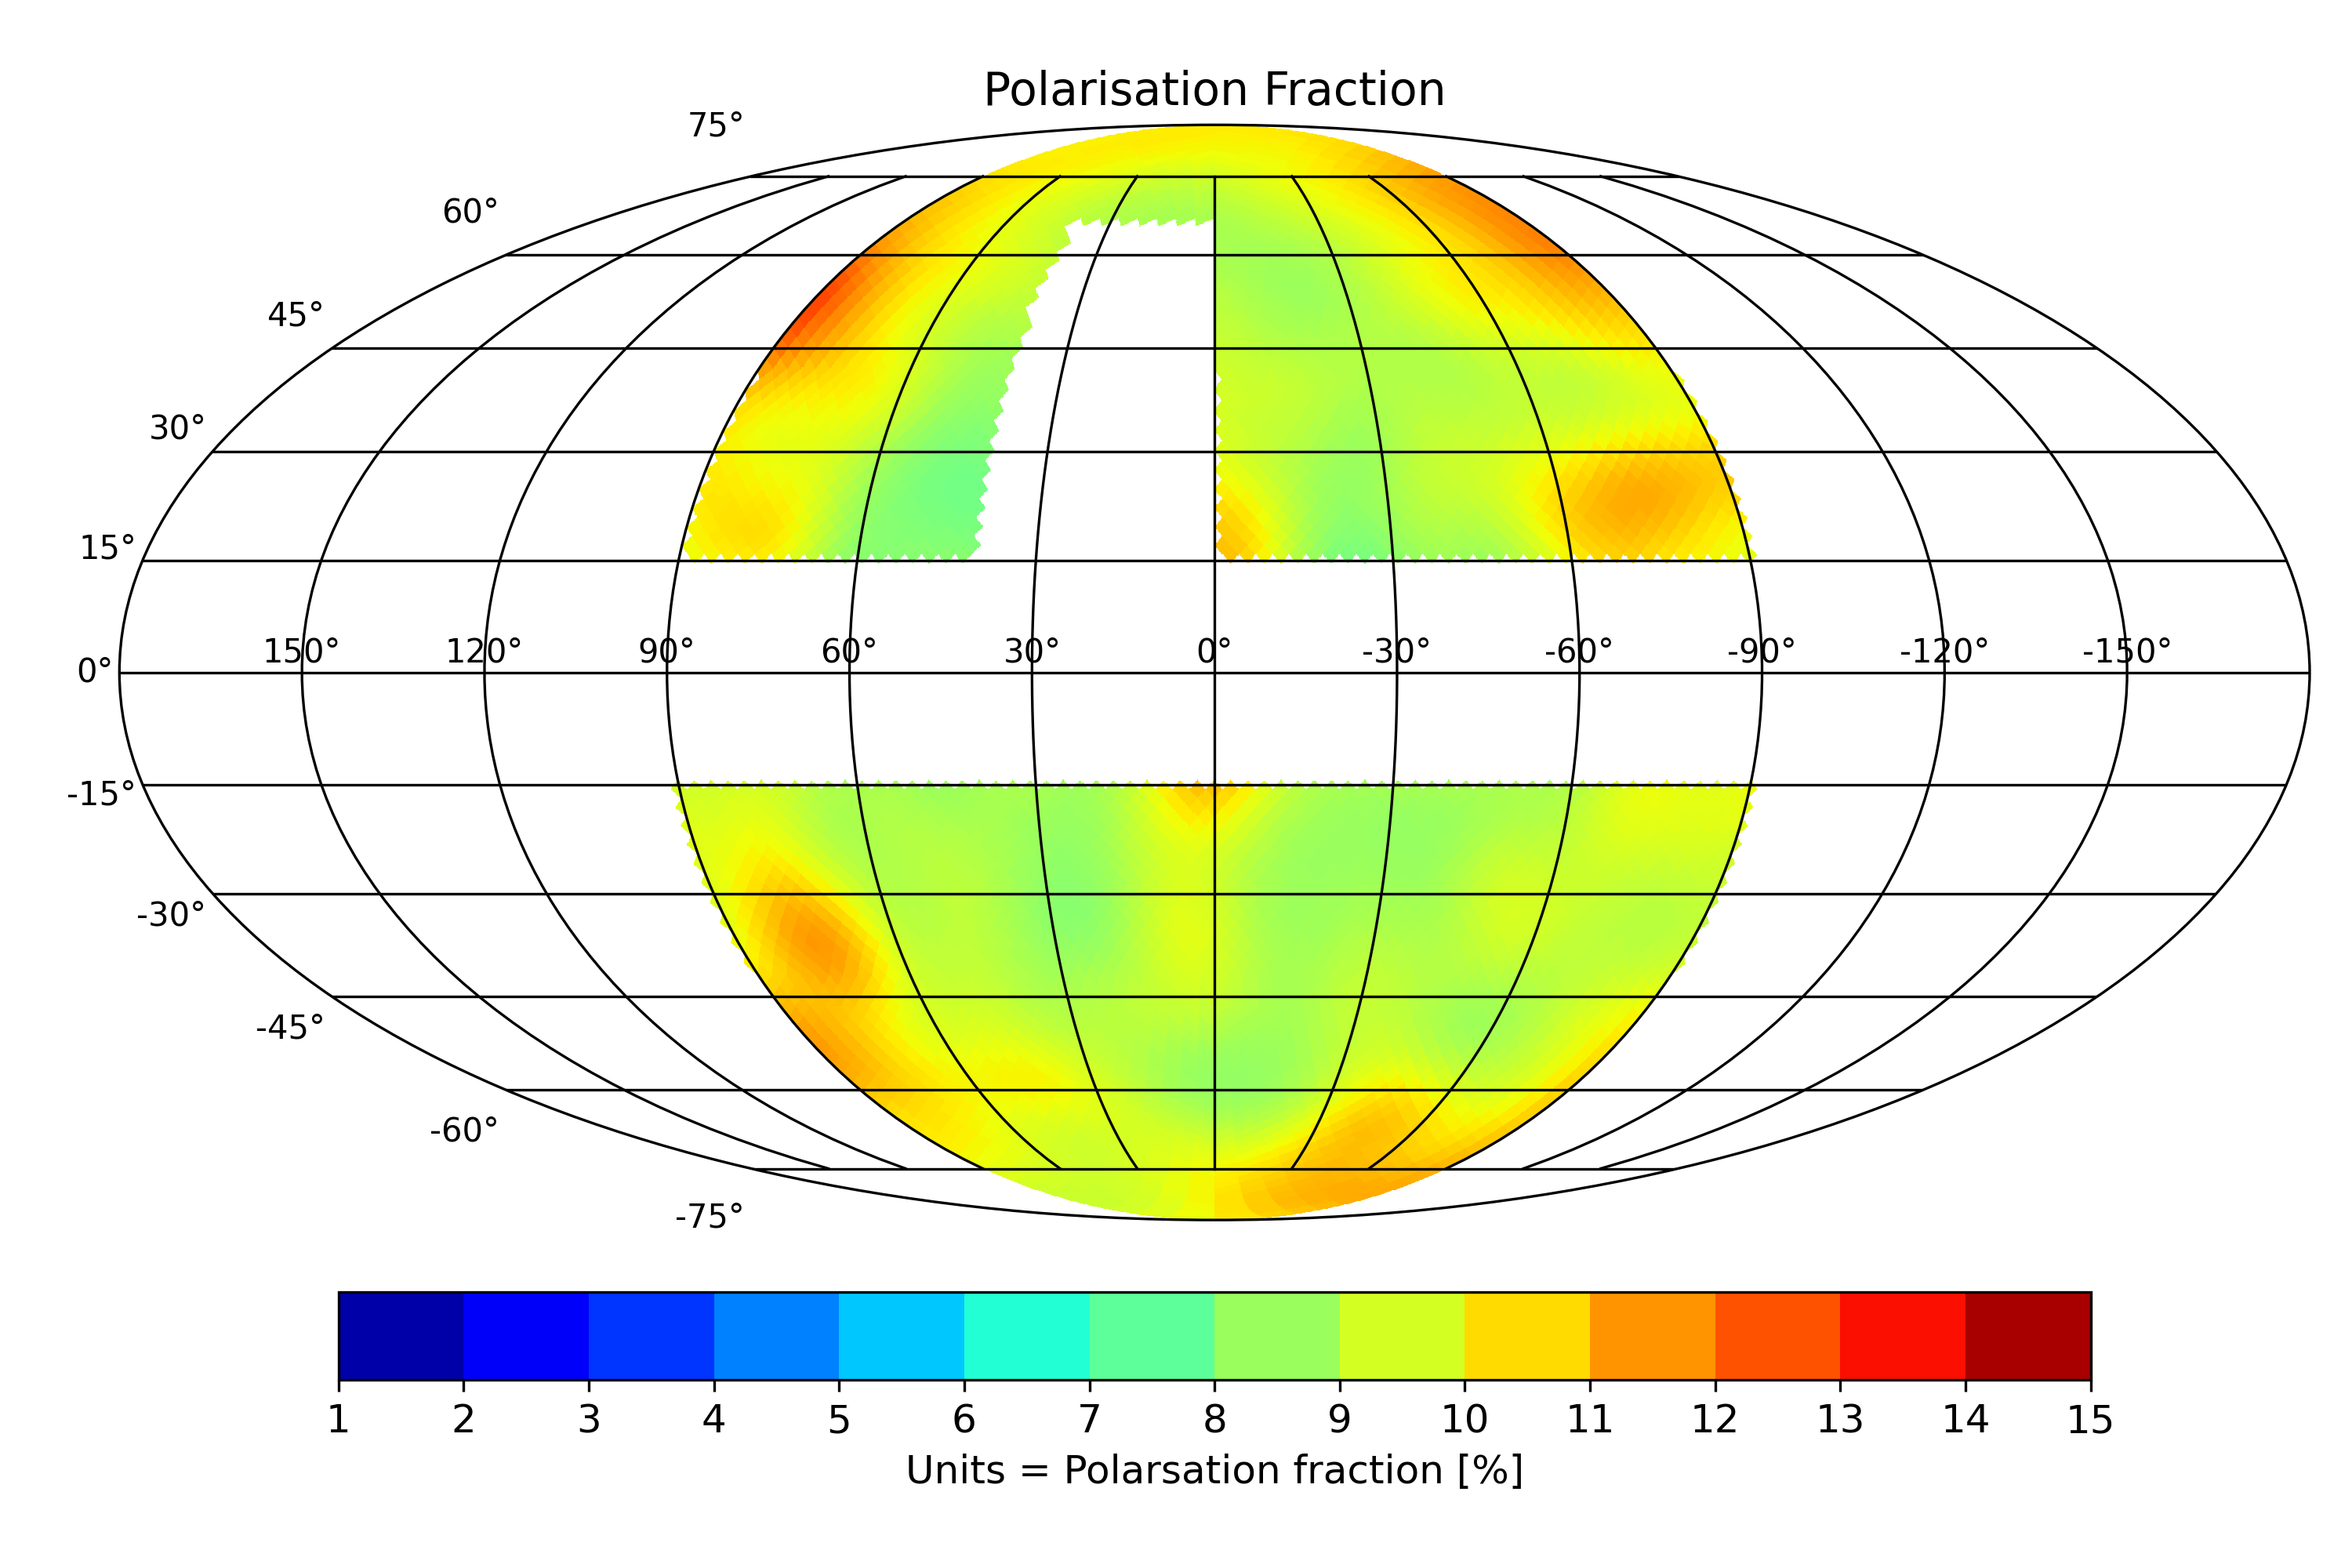
\includegraphics[width =0.49\linewidth]{Images/Jan-20-2022_Pol_Frac_30GHz_Total_Skymap_Bstr_3_Btur_6_Rmag_5_Zmag_7_norm_-1.24e+01.png}
\caption{\textbf{Top:} Planck polarised emission (\textbf{left}) and simulated polarised emission skymap from best fit parameters (see table ~\ref{Para_table}). \textbf{Bottom:} Residual of observation and simulated data (\textbf{left}) and polarisation fraction for toy model (\textbf{right}).}
\label{fig:Skymaps}
\end{figure*}

%\newpage

%% Uncertainities in the parameters

\begin{table*}
\centering
\caption{Table of best fit parameters with uncertainties}
\begin{tabular}{ |p{4.cm}|p{4.5cm}|p{6.5cm}|  }
\hline
\multicolumn{3}{|c|}{Best-fit value with 1-$\sigma$ constraint} \\
\hline
Parameter & Best-fit value &Description \\
\hline
\hline
$B_{\mathrm{str}} $& $3_{-1}^{+8} ~ \mu$G & Structured field strength \\
\hline
$B_{\mathrm{tur}} $& $ 6_{-2}^{+12} ~\mu$G & Turbulent field strength\\
\hline
$R_{\mathrm{Mag}}$ = $R_{\mathrm{el}}$ & $5_{-1}^{\infty}$~kpc & Radial cut off \\
\hline
$Z_{\mathrm{Mag}}$ = $Z_{\mathrm{el}}$ & $7_{-1}^{+1}$~kpc & Azimuthal cut\\
\hline
\rule{0pt}{3ex} 
${\rm{log_{10}}}(C_{\rm norm} [{\rm cm}^{-3}]$) & ${-12.43}_{{-1.31}}^{{+0.32}}$ & Electron normalisation at 10~GeV\\
\hline
\end{tabular}
\label{Para_table}
\end{table*}

% \section{Cosmic ray deflections from different magnetic field models}
\section{Cosmic ray deflections from magnetic field model range}
\label{Deflections}

When charged particles propagate through magnetic fields, they precess around the field lines by virtue of the Lorentz force 
\begin{eqnarray}
\frac{{\rm d}\bfm{\beta}}{c{\rm d}t} = \frac{1}{r_{L}}\bfm{\beta}\times \bfm{\hat{B}}, 
\end{eqnarray}
where $\bfm{\beta}$ is the particle's velocity vector, and $r_{L}$ is the particle's Larmor radius. UHECRs undergo the same Lorentz force when propagating through Galactic magnetic fields. The extra-Galactic magnetic field is considered to be weak, with $B < \rm {nG}$ for $\lambda_{\rm coh}=1$~Mpc \cite{Barrow_1997}, \cite{Kronberg_2007}, and the ultra-high energy cosmic rays UHECRs $E > 10^{19}$ EeV and subsequently $r_{L}>{\rm 10~Mpc}$ are therefore not sensitive to them over 10~Mpc propagation distance scales. However, once they enter the Galaxy magnetic fields are of the order of few $\mu$G. In case for a proton at 6~EeV in $6~\mu$G field the $r_L \approx 1 ~ \rm kpc$ , this implies that the proton will be subject to deflection by the large scale Galactic magnetic fields.

To propagate the cosmic rays we used the CRPropa3's \cite{CRPropa3_2016} Boris pusher scheme in order to ensure particle's trajectory evolution satisfies the Lorentz force equation. CRPropa conserves the total energy each particle during the propagation. 
To achieve this we backtrack $10^7$ cosmic rays starting isotropically from earth to a distance of 20~kpc. We use nitrogen as a choice of our cosmic ray particles at 40~EeV energy. 

\subsection{The Effect of Magnetic Field Model on UHECR Arrival}
In figure~\ref{fig:AD_Plots} we show, \textit{1)} the histogram of all sky in log (density/str) of the backtracked positions for the cosmic rays (\textbf{left}), there are 180 bins both for longitudes and latitudes.\textit{2)} is the histogram of binned arrival directions of cosmic rays in a $5^{\circ}$ region from two known sources (\textbf{right}) Centaurus A (lat = $\rm 19.42^{\circ}$, lon = $\rm 50.49^{\circ}$) and NGC 253 (lat = $\rm -87.96^{\circ}$, lon = $\rm 97.36^{\circ}$).  We normalise both the skymaps with first making histograms with no-magnetic fields and then dividing the histogram generated using toy model by the former. This gives us a normalised value of the number of hits obtained as seen on the right in the figure~\ref{fig:AD_Plots}.

It can be seen that the best fit and lower extreme parameters can clearly help in associating the deflected particles with their potential source. However, in the case of upper extreme parameters any connection between the point of origin of cosmic rays and their final positions is inconclusive. Cosmic rays from  sources like NGC253 get completely deflected by the magnetic field and hence we obtain a suppressed flux $\approx 5\%$ . In case of Centaurus A the final positions are spread out on the entire sky making it impossible to associate it with the source. In table~{\ref{AD_table}} we show the 
%%%%%%%%%%%%%%%%%%%%%%%%%%%%%%%%%%%%%%%%%%%%%%%%%%%%%%%%%%%%%%%%%%%%%%%%%%%%%%%%%%%%%%%%%%%%%%%%%%%%%%%%%%%%%%
%%% Lower Bound

%%% NGC253 mean lat = -60.90231798341981 and lon = -9.43559404135401 degrees
%%% NGC253 standard deviation lat = 15.69753500376699 and lon = 84.34462835618804 degrres
%%% NGC253 variance lat = 0.07506157199726642 and lon = 2.167053299539898

%%% CenA mean lat = 14.137807893047896 and lon = 39.59795385602137 degrees
%%% CenA standard deviation lat = 22.427737611940568 and lon = 26.033548777265693 degrees
%%% CenA variance lat = 0.15322360223540268 and lon = 0.20645313481127128

%%%%%%%%%%%%%%%%%%%%%%%%%%%%%%%%%%%%%%%%%%%%%%%%%%%%%%%%%%%%%%%%%%%%%%%%%%%%%%%%%%%%%%%%%%%%%%%%%%%%%%%%%%%%%%
%%% Upper Bound

%%% NGC253 mean lat = -2.322388780731066 and lon = -8.664927316867324 degrees
%%% NGC253 standard deviation lat = 39.046039934810125 and lon = 98.20089826558244 degrees
%%% NGC253 variance lat = 0.46441765734531754 and lon = 2.937552627840132

%%% CenA mean lat = 0.33584693428469714 and lon = 32.07788442314936 degrees
%%% CenA standard deviation lat = 38.066520277742804 and lon = 83.47296062758137 degrees
%%% CenA variance lat = 0.44140890797613463 and lon = 2.1224935049576783

%%%%%%%%%%%%%%%%%%%%%%%%%%%%%%%%%%%%%%%%%%%%%%%%%%%%%%%%%%%%%%%%%%%%%%%%%%%%%%%%%%%%%%%%%%%%%%%%%%%%%%%%%%%%%%
%%% Best Fit

%%% NGC253 mean lat = -48.890861373380375 and lon = -1.3601224872785176 degrees
%%% NGC253 standard deviation lat = 22.865215337703397 and lon = 83.981593692422 degrees
%%% NGC253 variance lat = 0.15925949224439517 and lon = 2.1484386610540773

%%% CenA mean lat = 8.648647356708622 and lon = 45.80995936362569 degrees
%%% CenA standard deviation lat = 28.67183426567853 and lon = 35.674397052936385 degrees
%%% CenA variance lat = 0.2504180851714255 and lon = 0.3876751990217161
%%%%%%%%%%%%%%%%%%%%%%%%%%%%%%%%%%%%%%%%%%%%%%%%%%%%%%%%%%%%%%%%%%%%%%%%%%%%%%%%%%%%%%%%%%%%%%%%%%%%%%%%%%%%%%

%\begin{center}
\begin{table*}
\centering
\caption{CAPTION TEXT GOES HERE}
\begin{tabular}{|p{3.cm}|p{4.cm}|p{4.cm}|p{4.cm}|}
    \hline
    Parameter set & Mean (${}^\circ$)& SD (${}^\circ$) & Variance ($str$)\\
    \hline
    \multicolumn{4}{|c|}{Cen A} \\ 
    \hline
    \rule{0pt}{3ex} 
    Best Fit & $\overline{b} = 8.64$, $\overline{l} = 45.80 $& $\sigma_{b} = 28.67 $, $\sigma_{l} = 35.67$ & $\sigma^2_{b} = 0.25 $, $\sigma^2_{l} = 0.38$ \\
    \hline
    \rule{0pt}{3ex} 
     Lower & $\overline{b} = 14.13$  , $\overline{l} = 39.59$ & $\sigma_{b} = 22.42$, $\sigma_{l} = 26.03$ & $\sigma^2_{b} = 0.15 $, $\sigma^2_{l} = 0.20$\\
    \hline
    \rule{0pt}{3ex} 
     Upper & $\overline{b} = 0.33$, $\overline{l} = 32.07$ & $\sigma_{b} = 38.06$ , $\sigma_{l} = 83.47$ & $\sigma^2_{b} = 0.44 $, $\sigma^2_{l} = 2.12$\\
    \hline
  \multicolumn{4}{|c|}{NGC 253} \\ 
    \hline
    \rule{0pt}{3ex} 
    Best Fit & $\overline{b} = -48.89$, $\overline{l} = -1.36$  & $\sigma_{b} = 22.86$ , $\sigma_{l} = 83.98$ & $\sigma^2_{b} = 0.15 $, $\sigma^2_{l} = 2.14$ \\
    \hline
    \rule{0pt}{3ex} 
     Lower & $\overline{b} = -60.90 $, $\overline{l} = -9.43$ & $\sigma_{b} = 15.69$, $\sigma_{l} = 84.34 $ & $\sigma^2_{b} = 0.07 $, $\sigma^2_{l} = 2.16$\\
    \hline
    \rule{0pt}{3ex} 
     Upper & $\overline{b} = -2.32$, $\overline{l} = -8.66$ & $\sigma_{b} = 39.04$ , $\sigma_{l} = 98.20 $& $\sigma^2_{b} = 0.44 $, $\sigma^2_{l} = 2.93$\\
    \hline
\end{tabular}
\label{AD_table}
\end{table*}

%\end{center}
%\newpage

\begin{figure*}
\centering
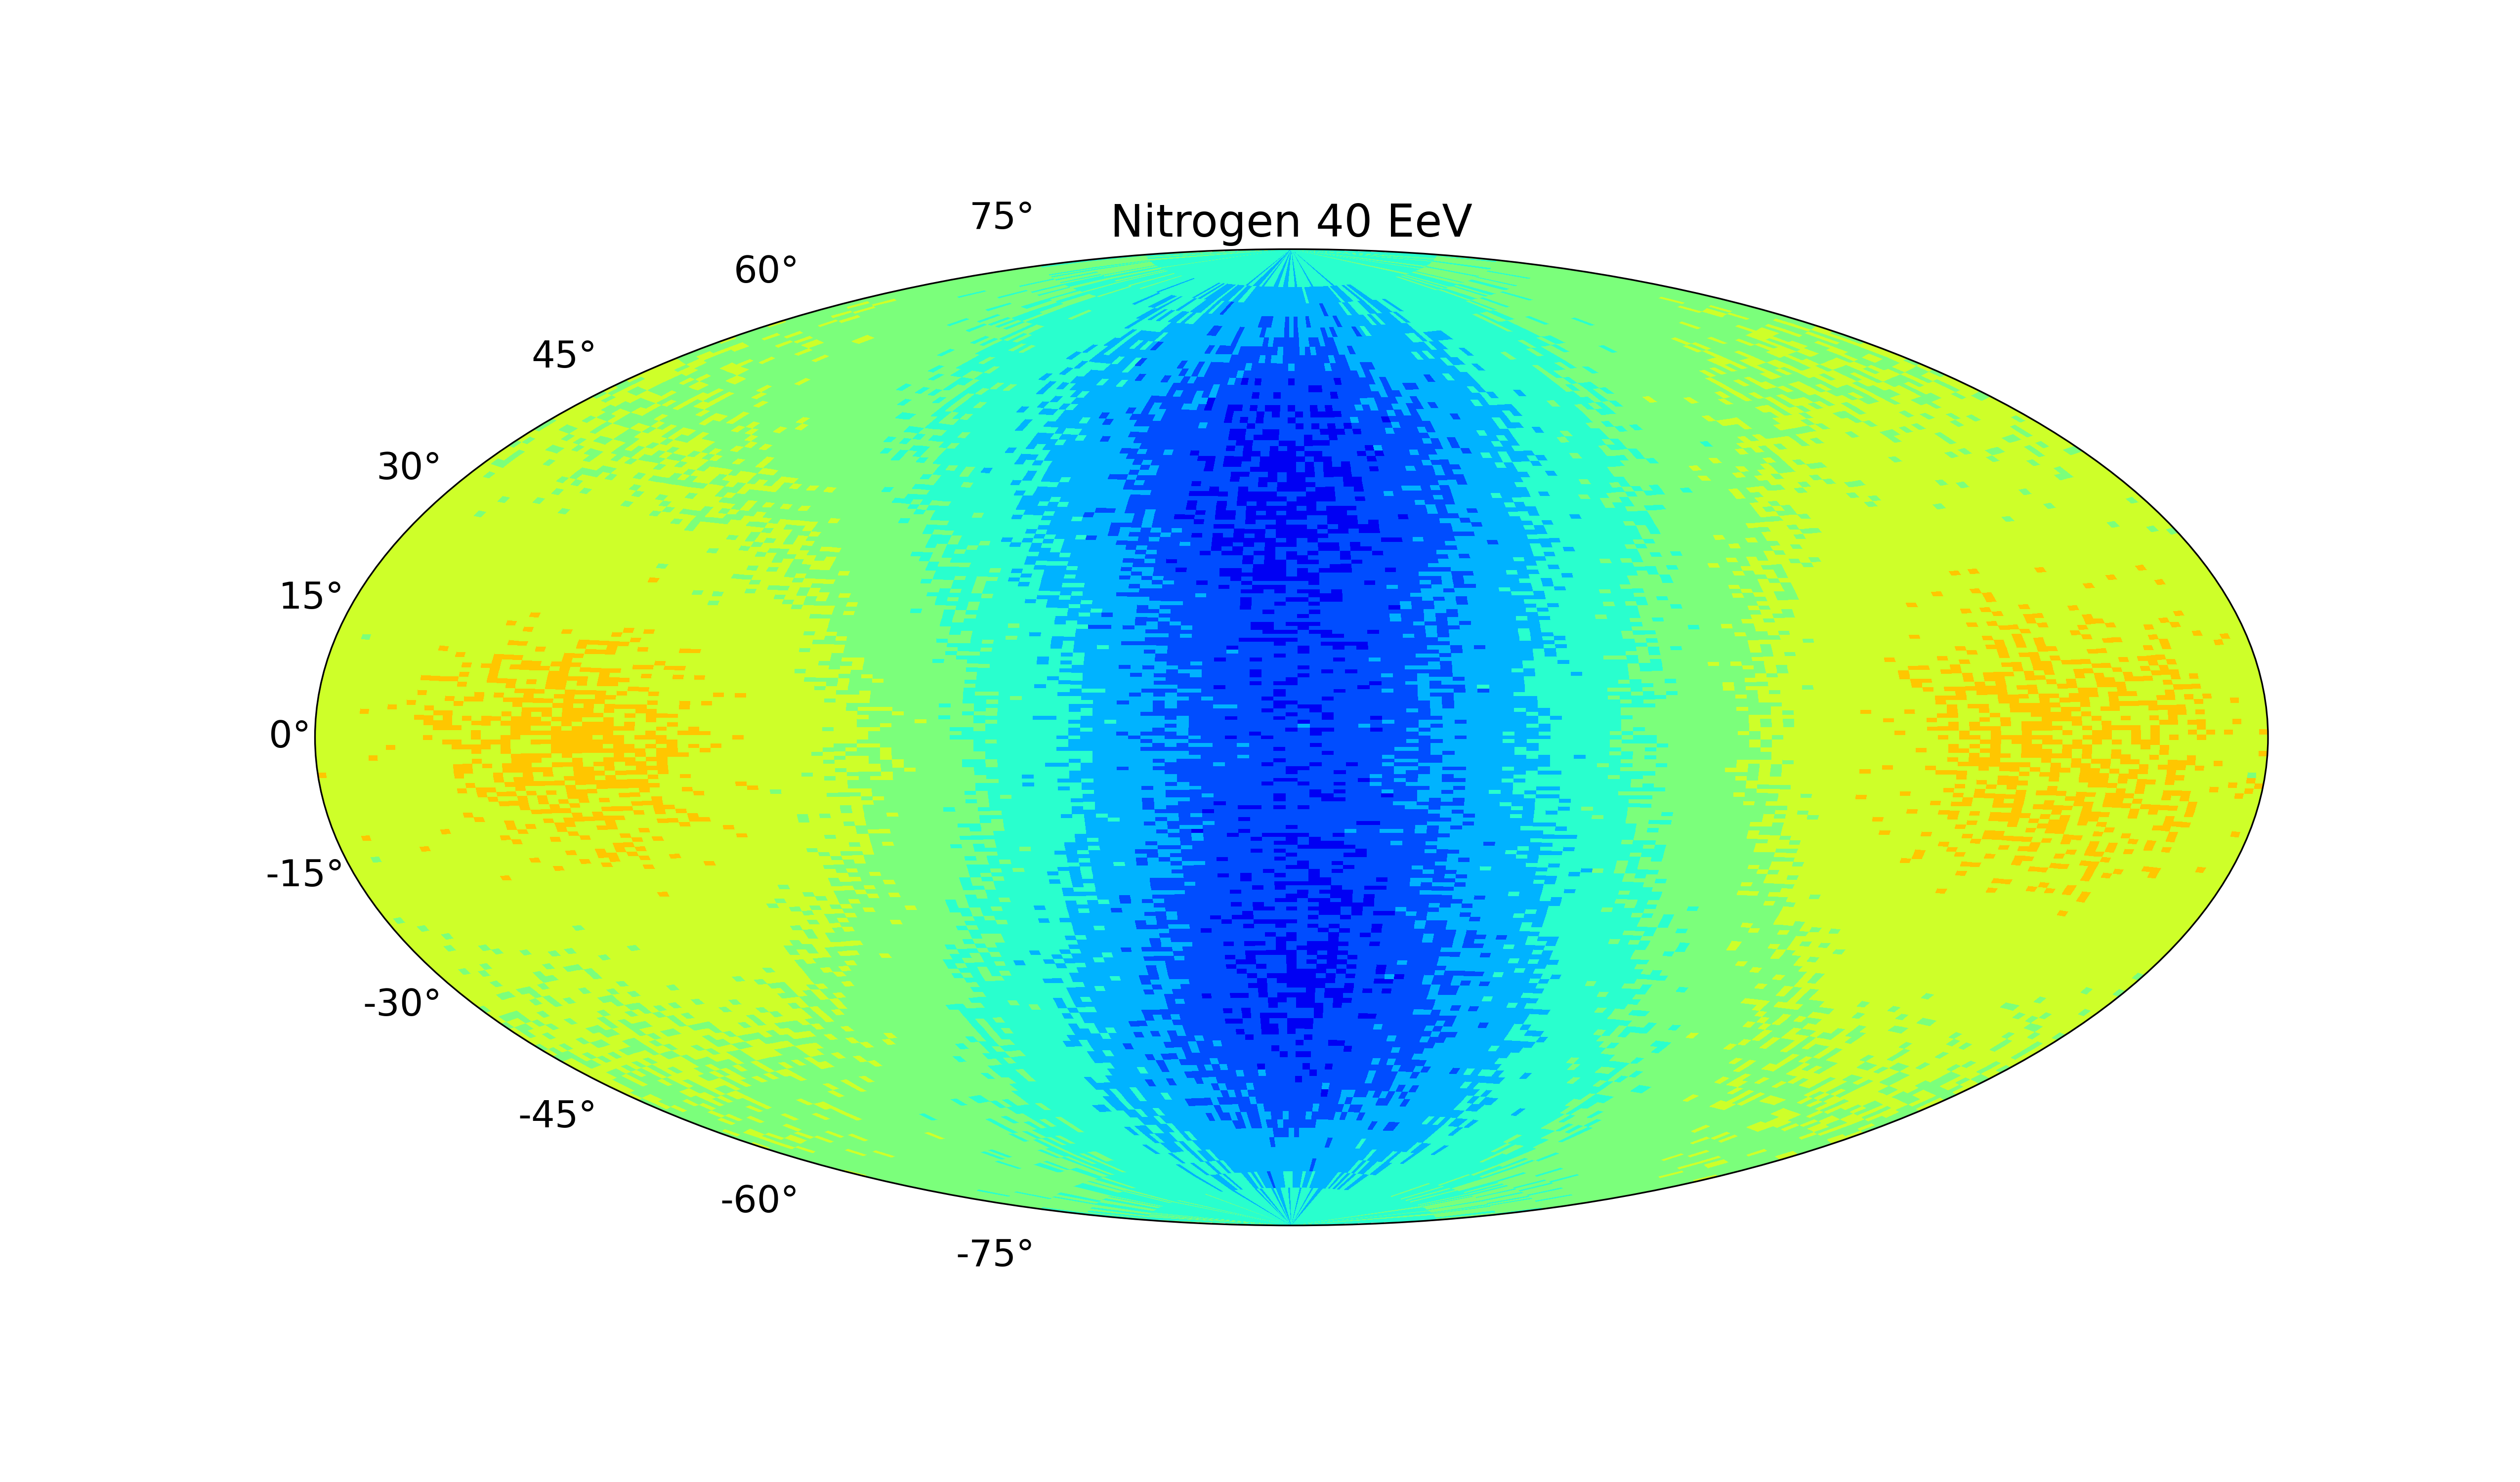
\includegraphics[width=0.49\linewidth]{Images/Log_Bins_180_Historgam_BF_N2_Str_Tur_TM_40_EeV.png}
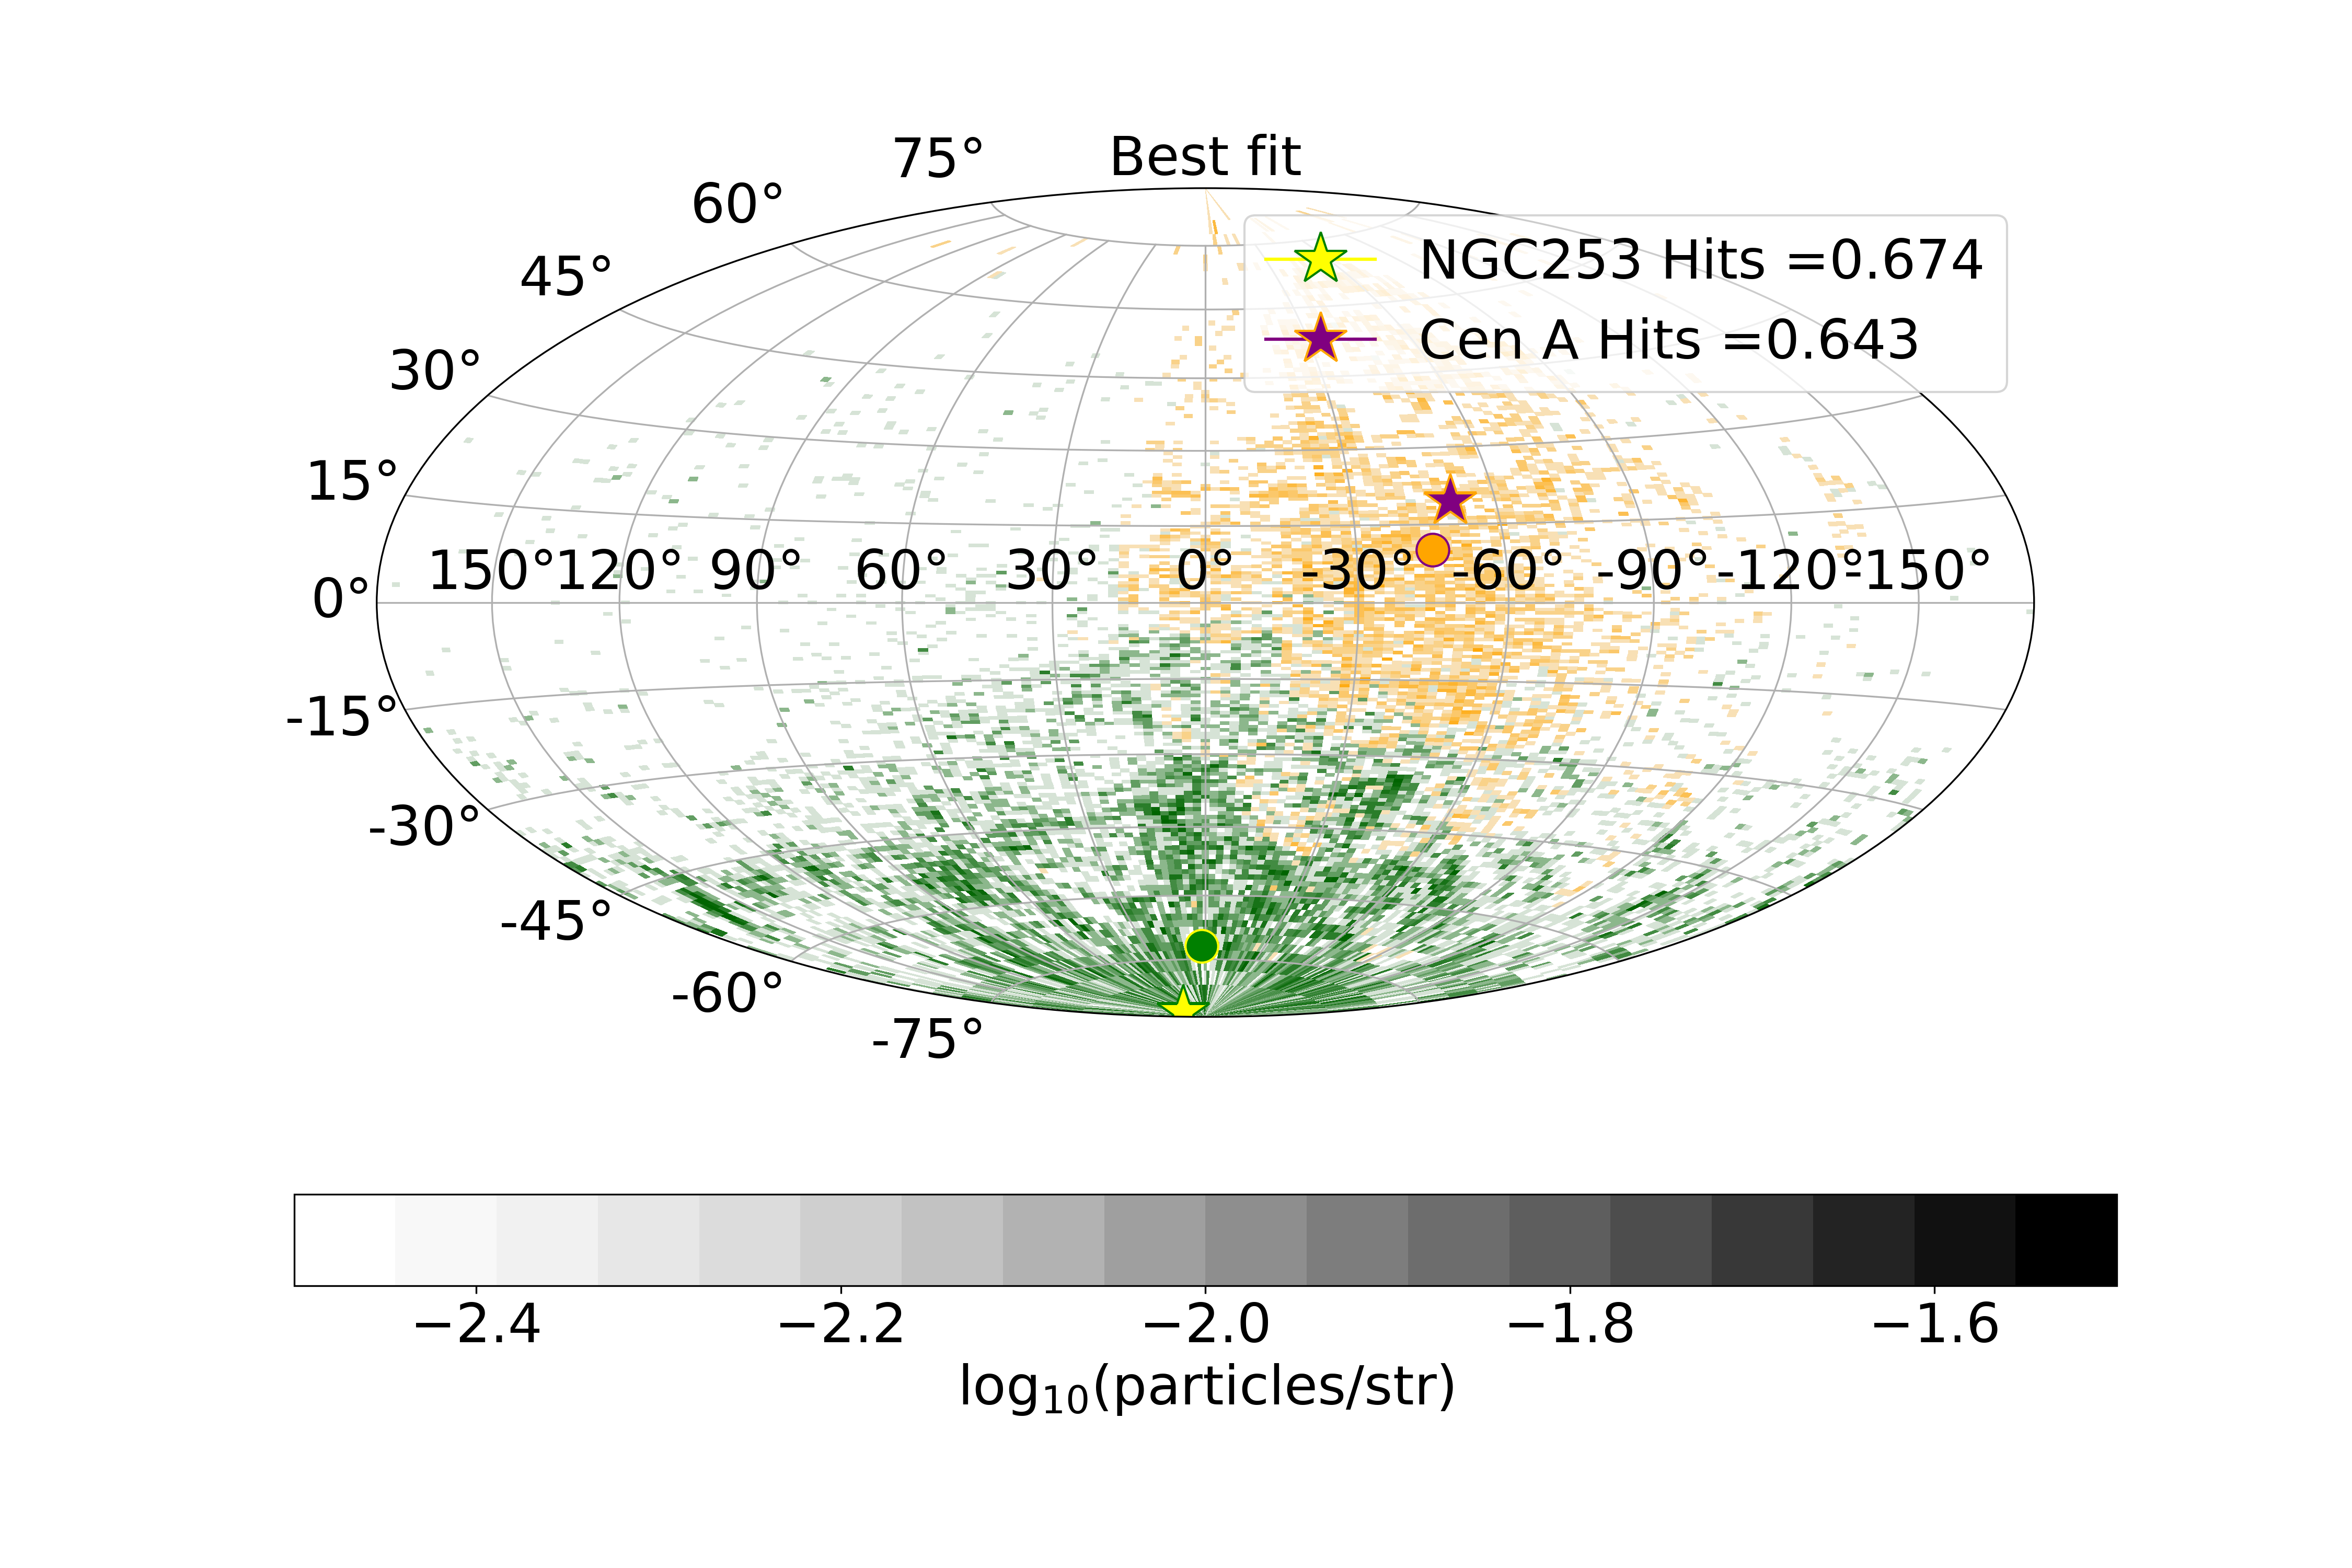
\includegraphics[width=0.49\linewidth]{Images/Bins_180_BF_N2_CenA_NGC253_Str_Tur_TM_40_EeV.png}\\
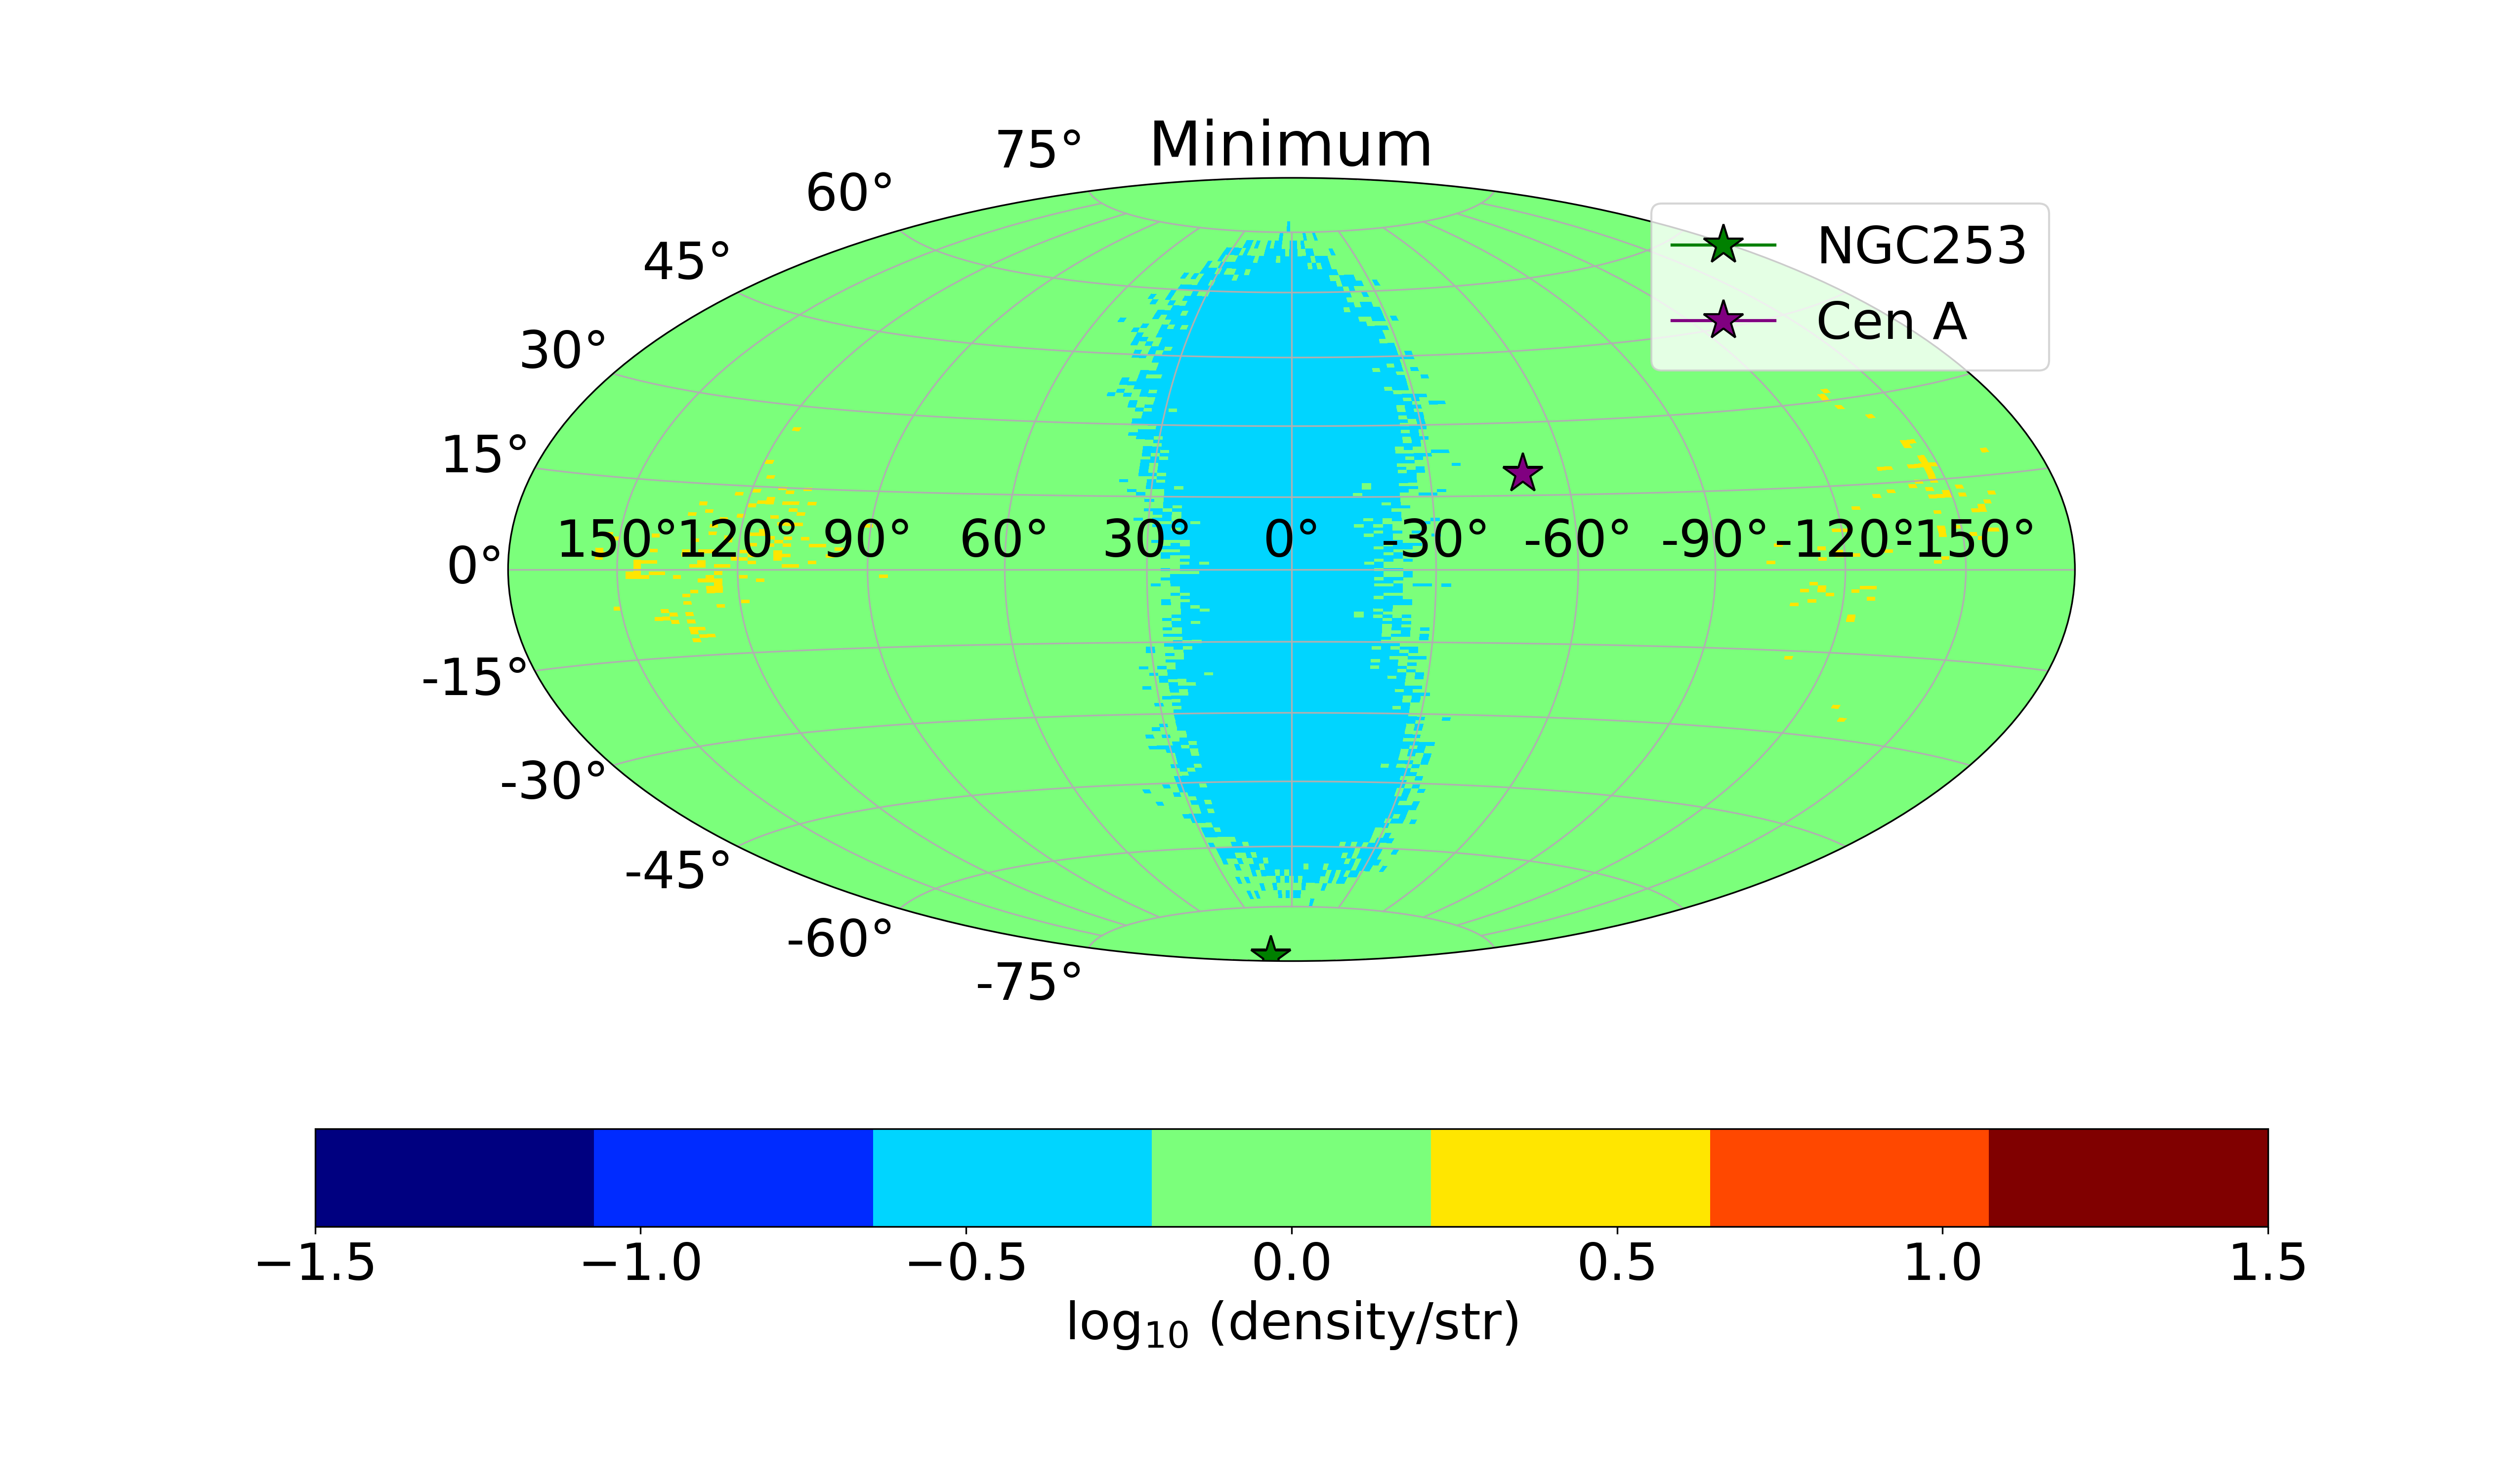
\includegraphics[width=0.49\linewidth]{Images/Log_Bins_180_Historgam_LB_N2_Str_Tur_TM_40_EeV.png}
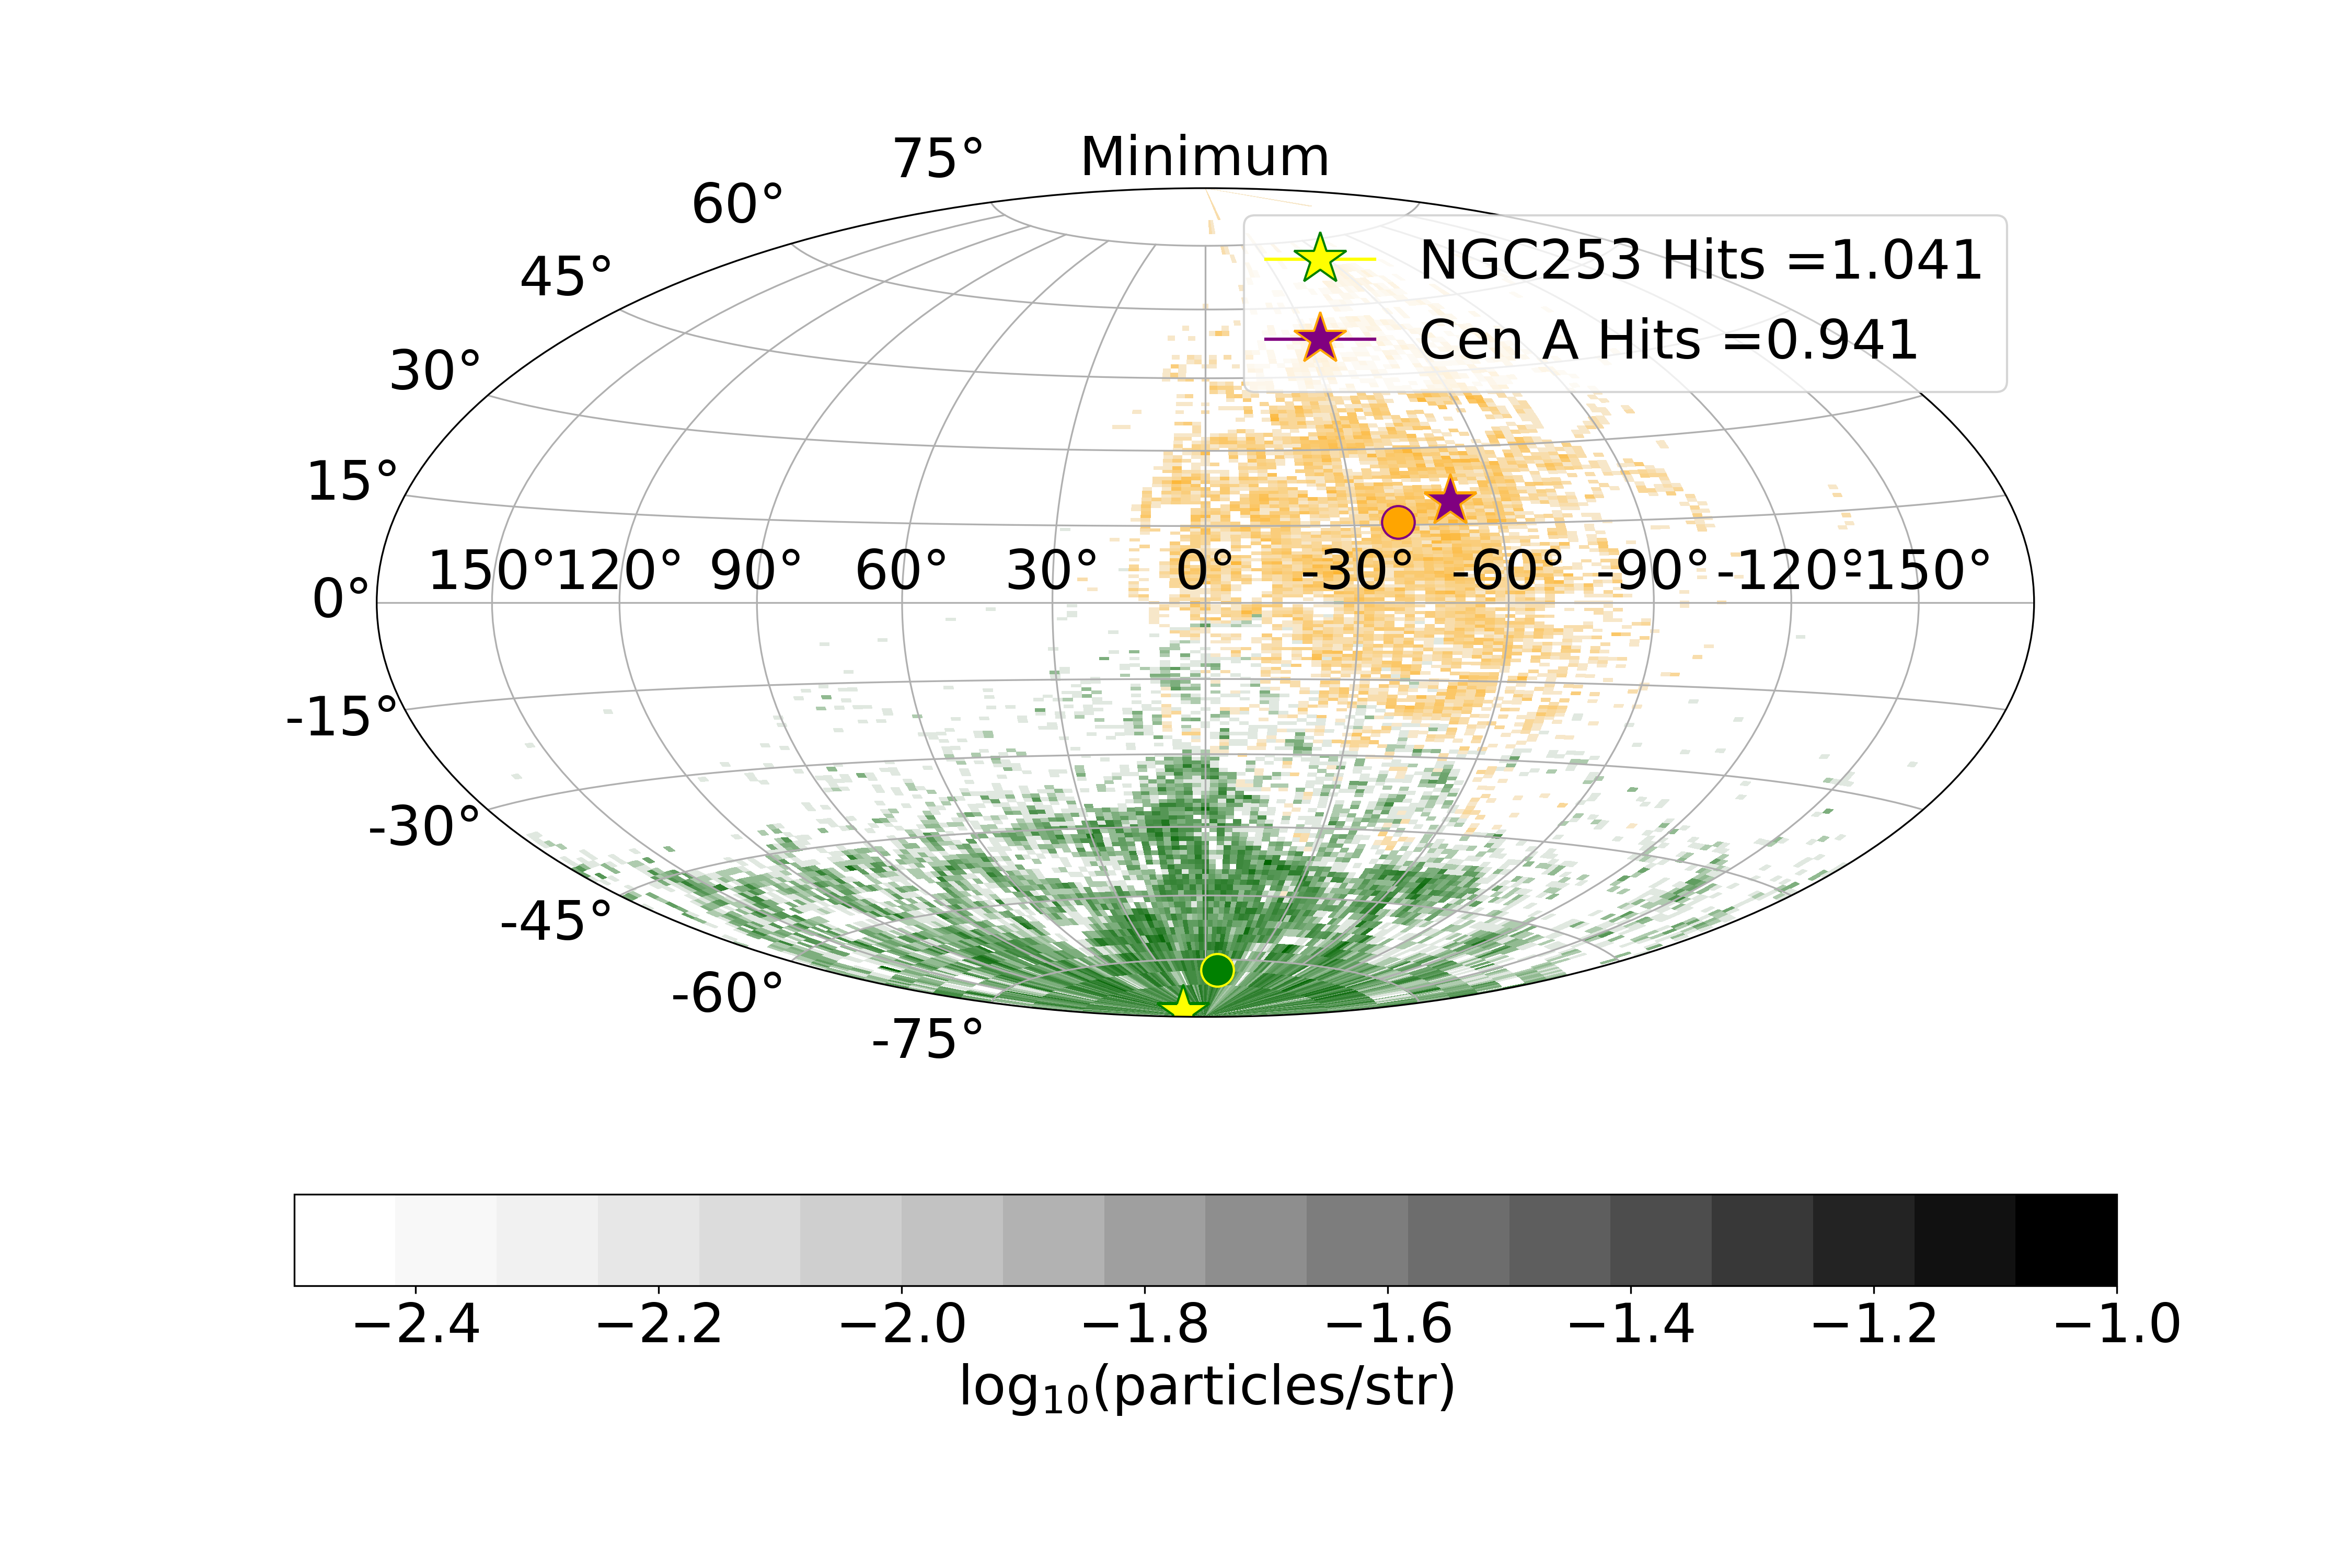
\includegraphics[width=0.49\linewidth]{Images/Bins_180_LB_N2_CenA_NGC253_Str_Tur_TM_40_EeV.png}\\
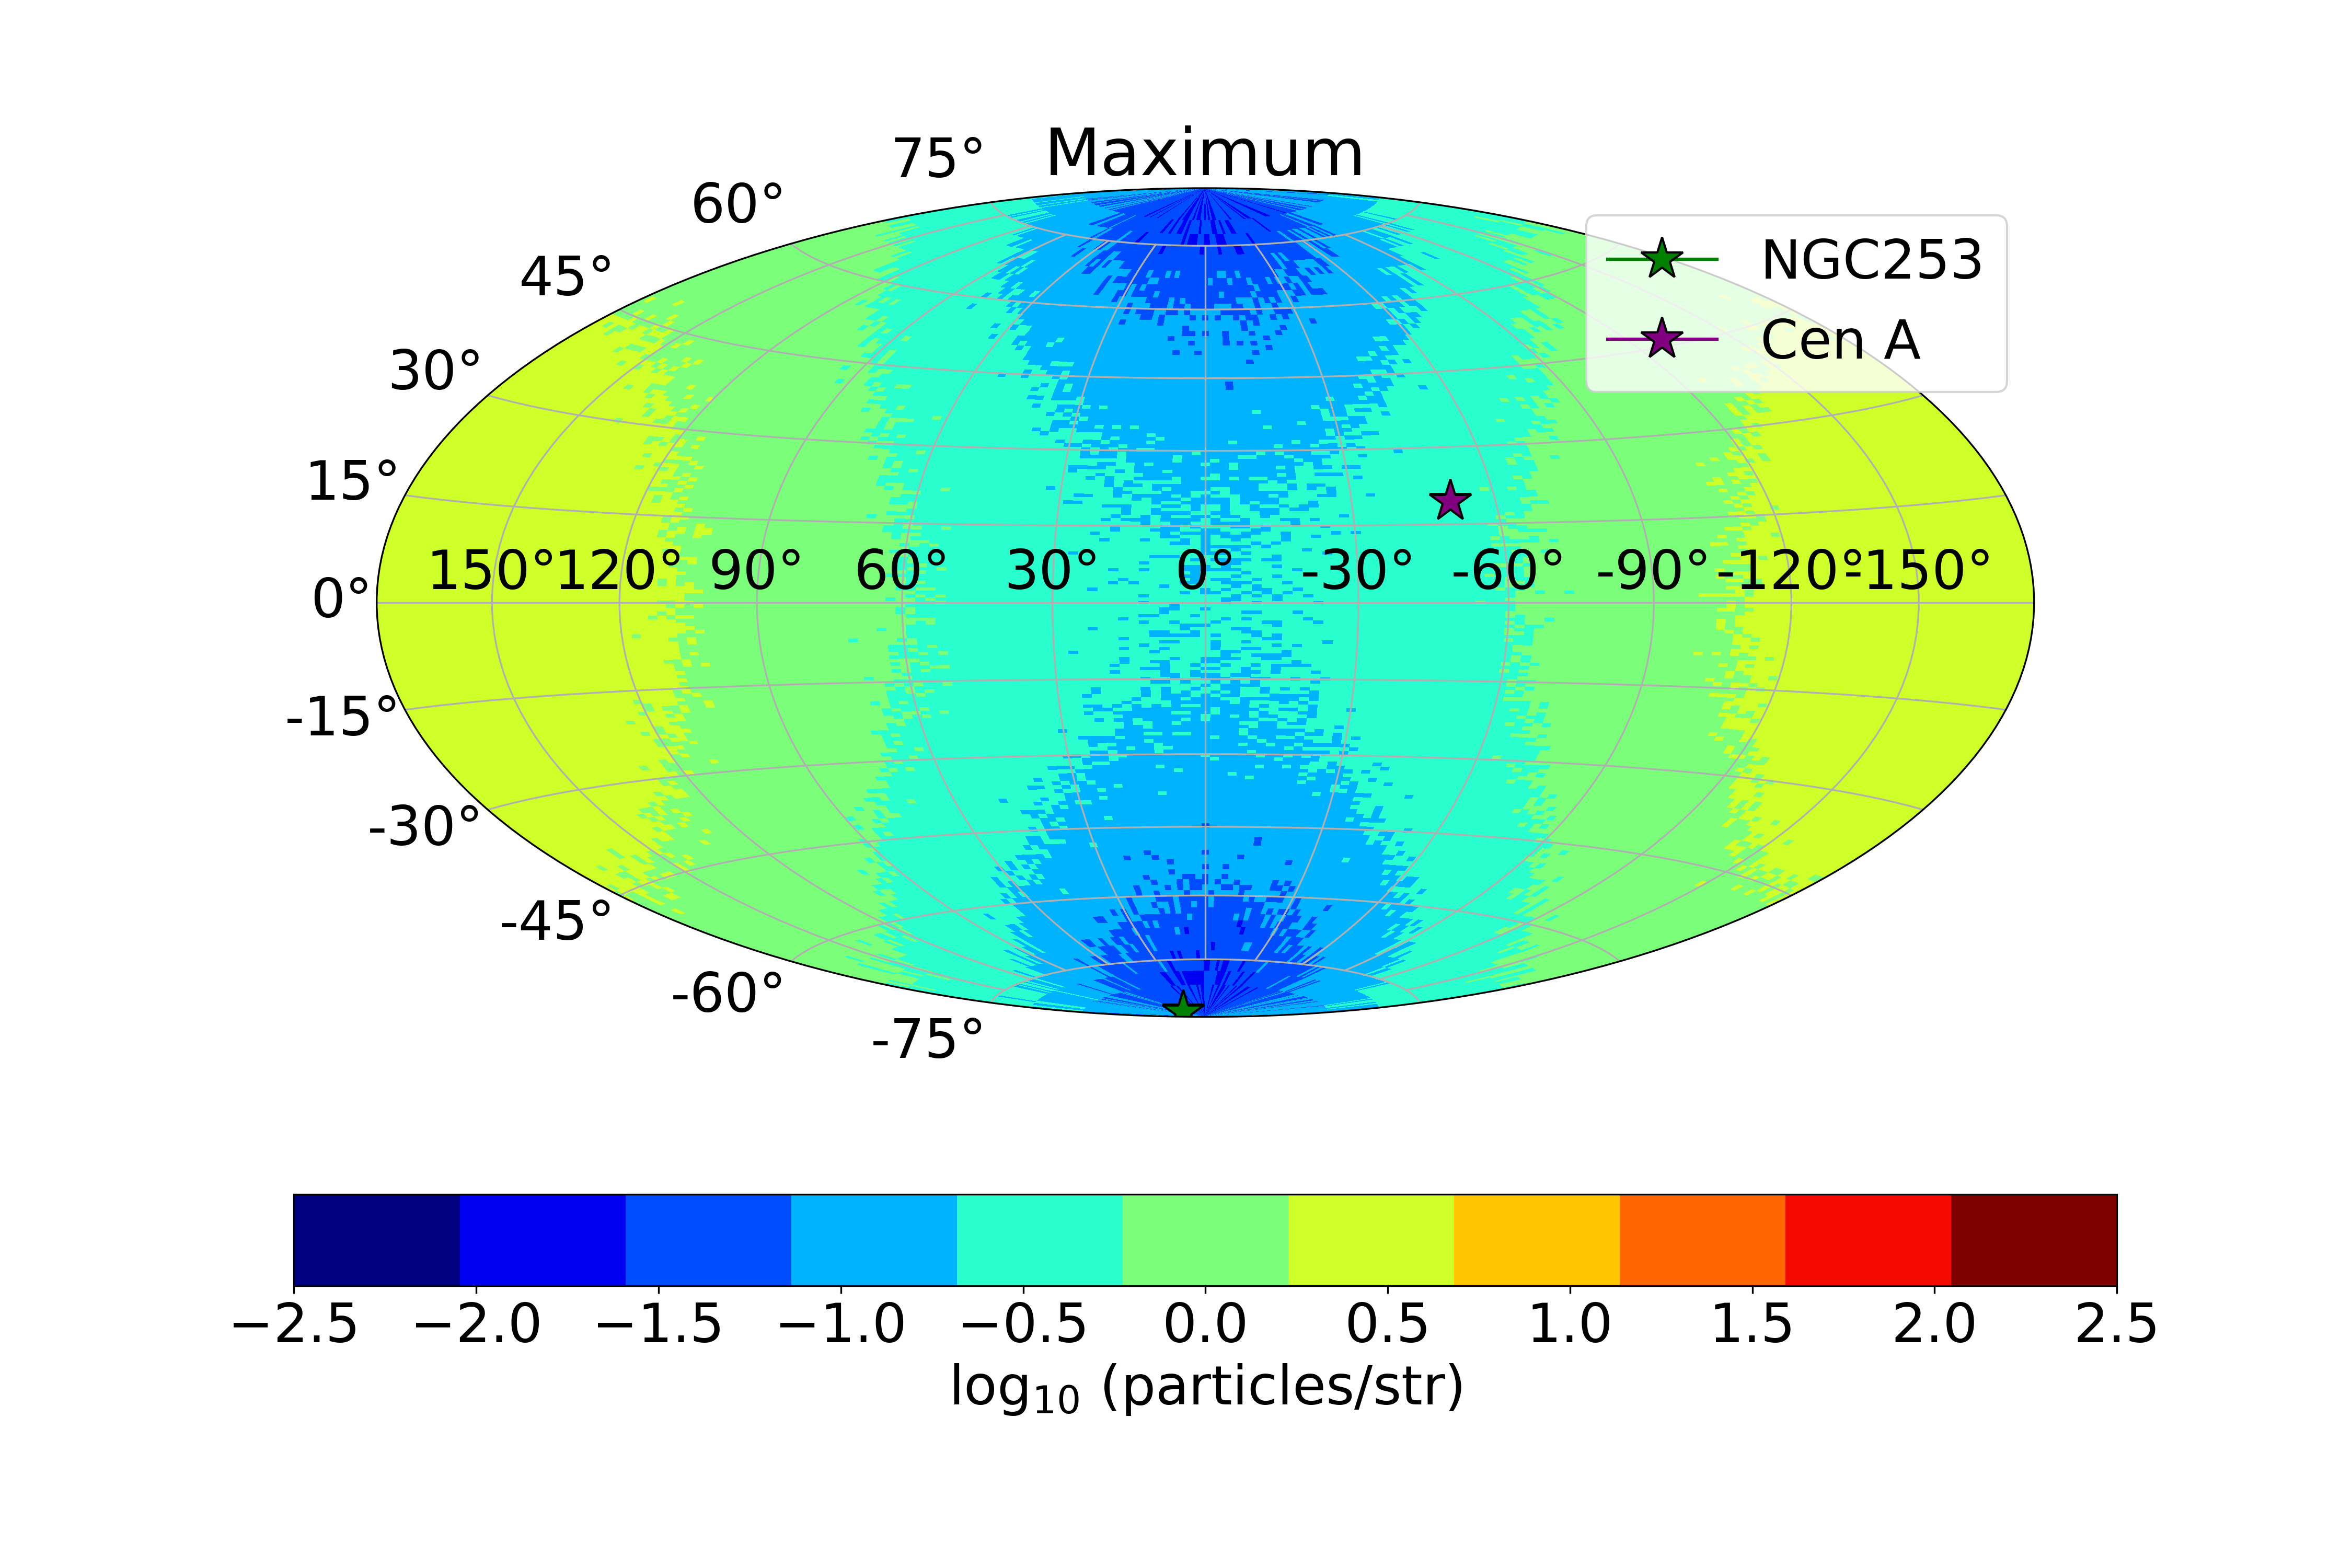
\includegraphics[width=0.49\linewidth]{Images/Log_Bins_180_Historgam_UB_N2_Str_Tur_TM_40_EeV.png}
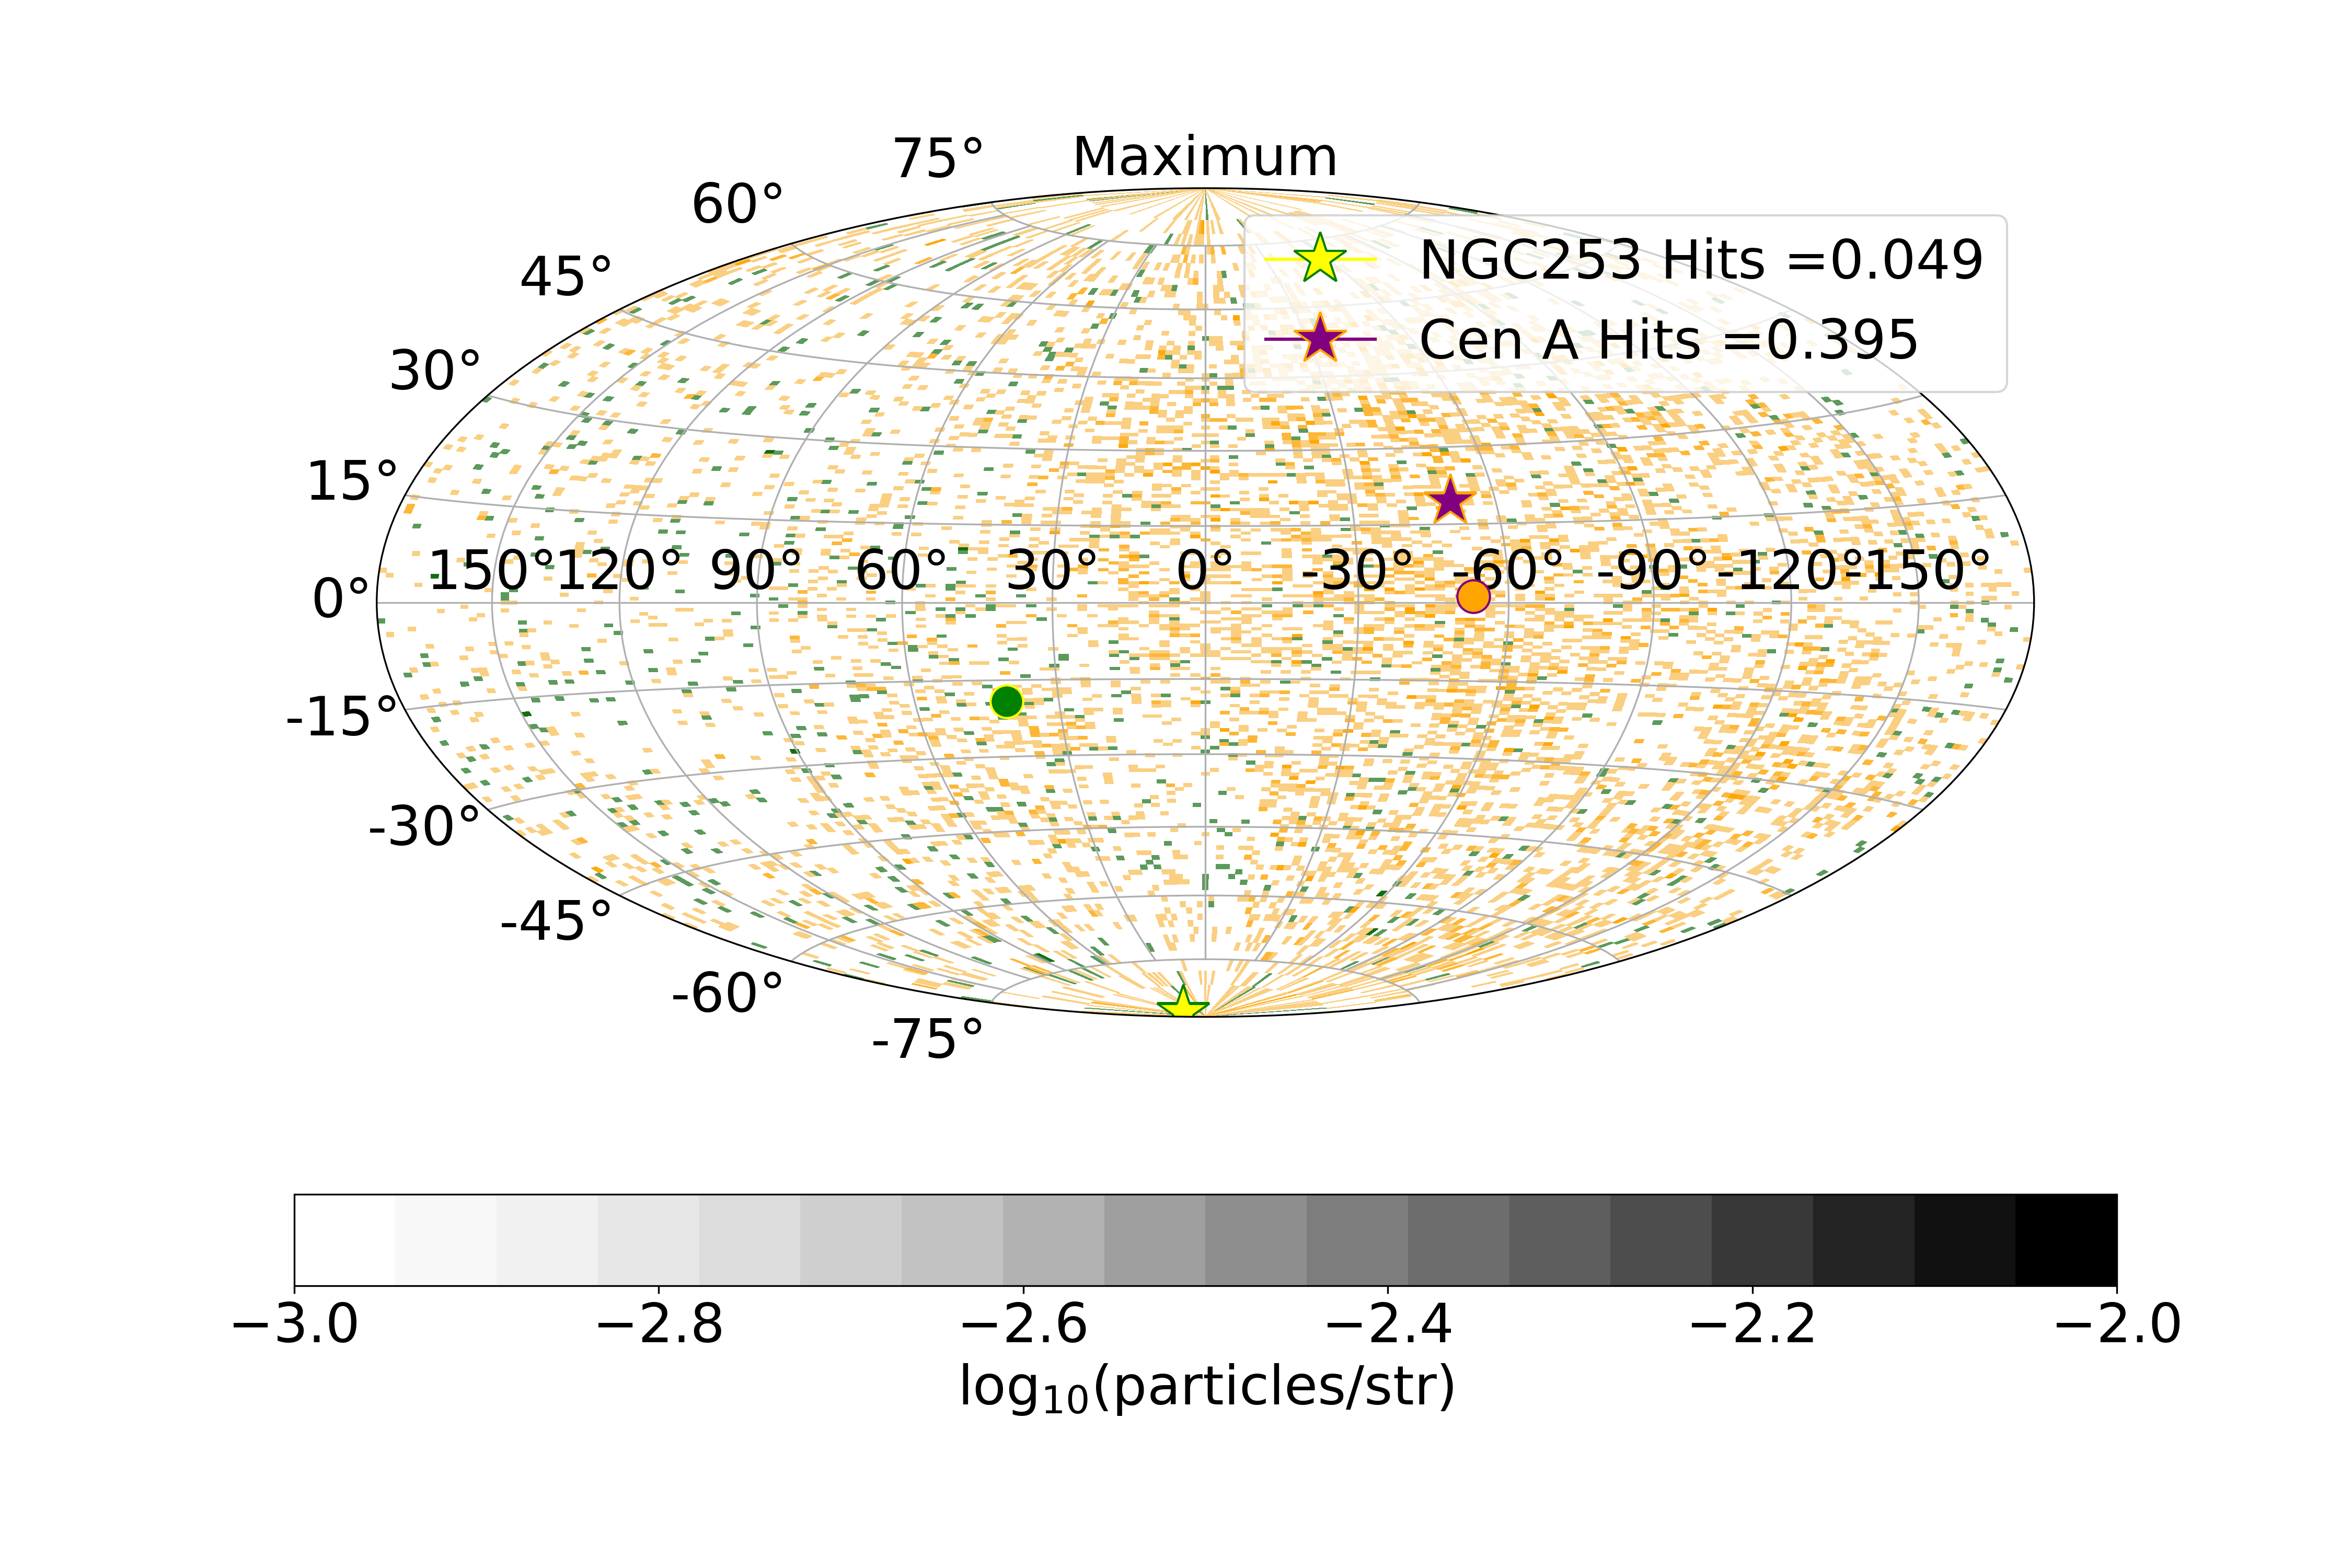
\includegraphics[width=0.49\linewidth]{Images/Bins_180_UB_N2_CenA_NGC253_Str_Tur_TM_40_EeV.png}
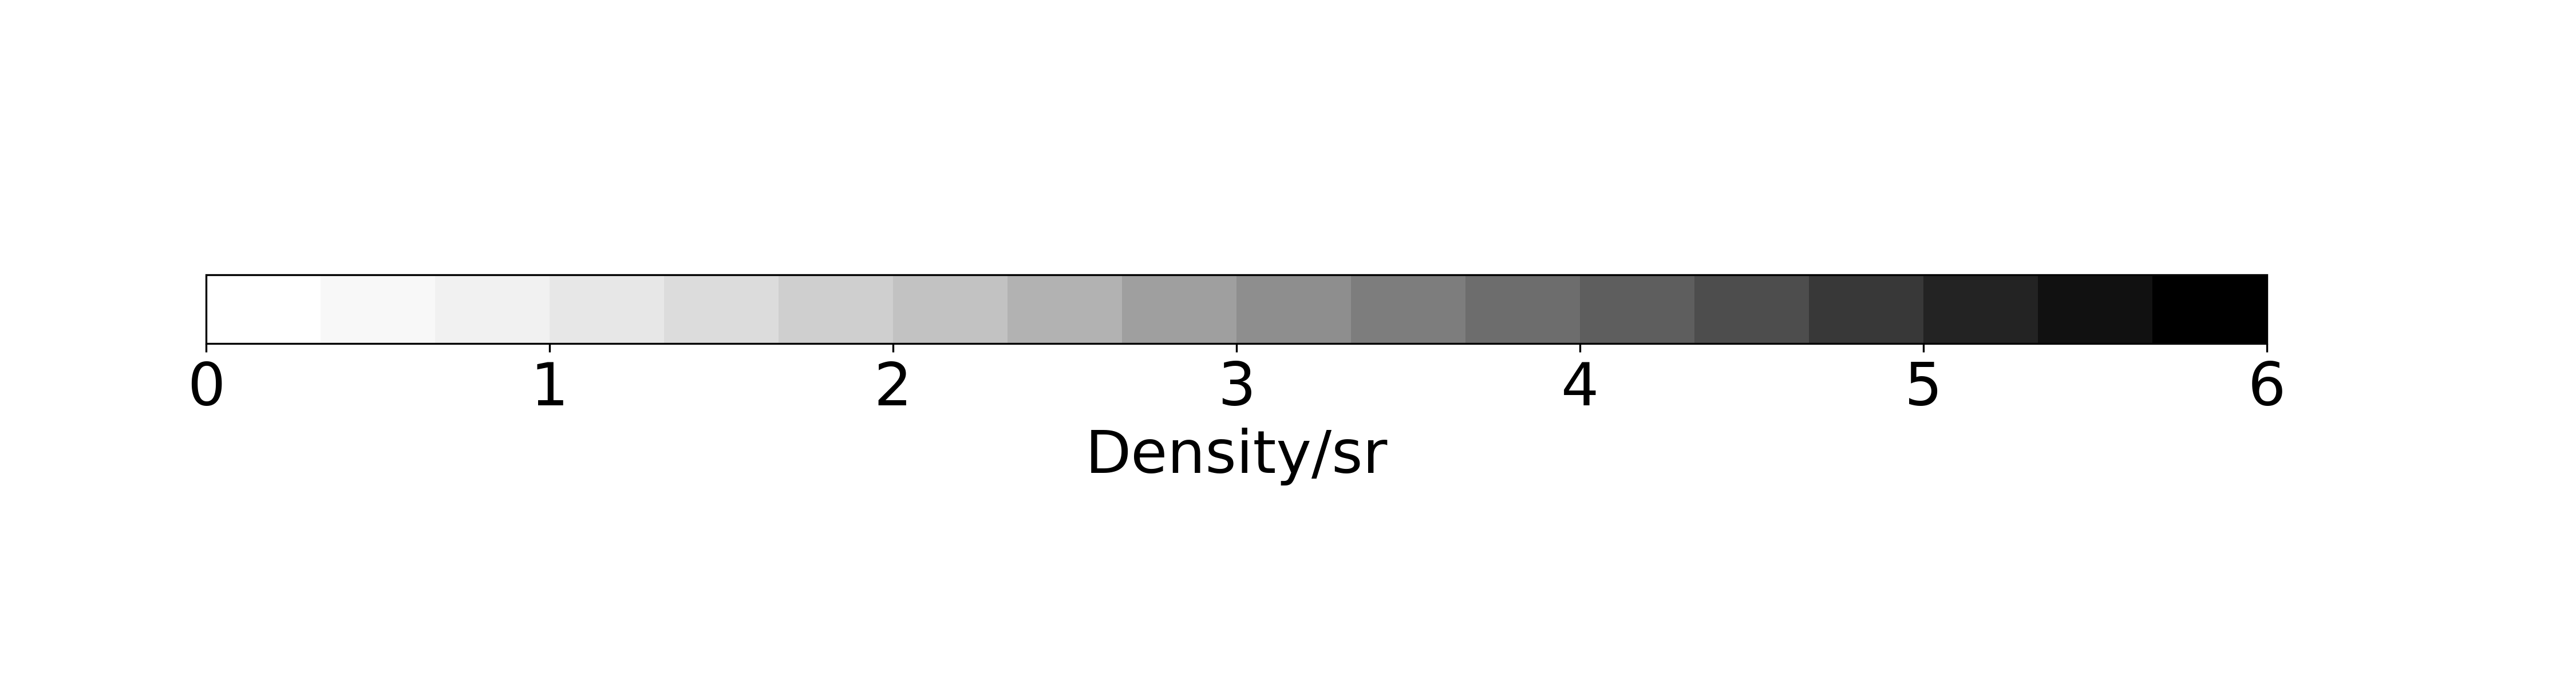
\includegraphics[width=0.49\linewidth]{Images/Colorbar.png}
\caption{Log brightness of the backtracked positions for cosmic rays shown on \textbf{left} and the arrival directions of the cosmic rays from two known sources Cen A and NGC 253 on \textbf{right} (From table~\ref{Para_table} \textbf{Top} - Best Fit Parameters, {\textbf{Middle} - Lower extreme parameters)} \& {\textbf{Bottom} - Upper extreme parameters, we use $R_{\rm Mag} = $ 20~kpc since that is the maximum extent of the magnetic fields in our simulation.}}
\label{fig:AD_Plots}
\end{figure*}
%\newpage

\section{Conclusions}
\label{Conclusions}

%\clearpage
\section{References}

%\printbibliography[heading=none]

\bibliographystyle{mnras}
\bibliography{references.bib}

\appendix

%\nocite{*}

In table ~\ref{Para_table} we provide the list of all free parameters and the constraints obtained on them.

\section{Polarised Synchrotron Emission}
\label{Appendix_A}
As discussed in section(\ref{Synchrotron_theory}) the line of sight components for Stokes parameters is given by:
\begin{eqnarray}
Q^l_{\rm in} = ({J_{\perp}^l} - J_{\parallel}^l) \ {\cos}(2\Psi^l_{\rm in}) \ \\ U^l_{\rm in} = ({J_{\perp}^l} - J_{\parallel}^l) \ {\sin}(2\Psi^l_{\rm in}) \ .
\end{eqnarray}
We can take two test cases (I \& II) given in figure(\ref{fig_tot_intensity}) and figure (\ref{fig_pol_intensity}) respectively.We consider that there are two steps along a line of sight for which ${J_{\perp}^{(1,2)}}$ = 0.85 and $J_{\parallel}^{(1,2)}$  = 0.15. 
\\ In case I the angles $\Psi_{\rm in}^{(1,2)}$ = $90^{\circ}$ \& $0^{\circ}$. The resultant value of $I_{\rm pol}$ = 0 by virtue of eq.(\ref{eq_I_pol}) and we only have a contribution in $I_{\rm tot}$. This implies that for case I the resultant emission is seen only in total intensity since the values of $J_{\perp}^{\rm tot}$ = $J_{\parallel}^{\rm tot}$. 
\\ In case II we apply similar calculations to case I however, now the angles are $\Psi_{\rm in}^{(1,2)}$ = $90^{\circ}$ \& $45^{\circ}$. This in turn results in contribution to both polarised emission $I_{\rm pol}$ and total intensity $I_{\rm tot}$. Thus the values of $J_{\perp}^{\rm tot} \neq J_{\parallel}^{\rm tot}$. In figure(\ref{fig_pol_intensity}) we only show polarised intensity for simplicity however, there will be both total intensity and polarised intensity present.
\begin{figure*}
     \centering
%     \begin{subfigure}{0.4\textwidth}
%         \centering
         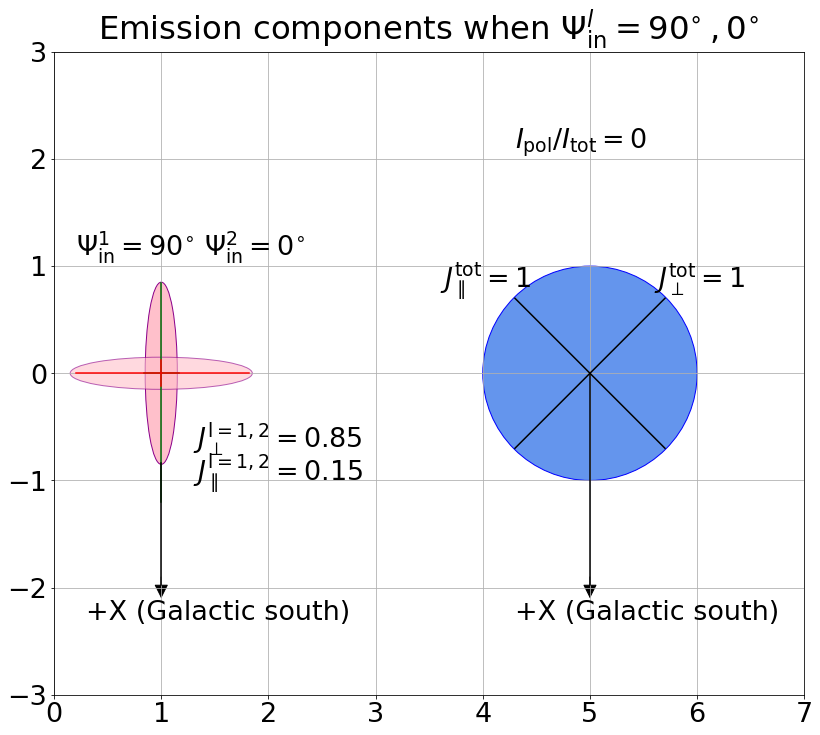
\includegraphics[width = 0.49\linewidth]{Images/Total_intensity_Ellipses_circles_emissions.png}
%         \caption{Case I - Total intensity}
%         \label{fig_tot_intensity}
%     \end{subfigure}
%  \hfill
%    \begin{subfigure}{0.4\textwidth}
%         \centering
         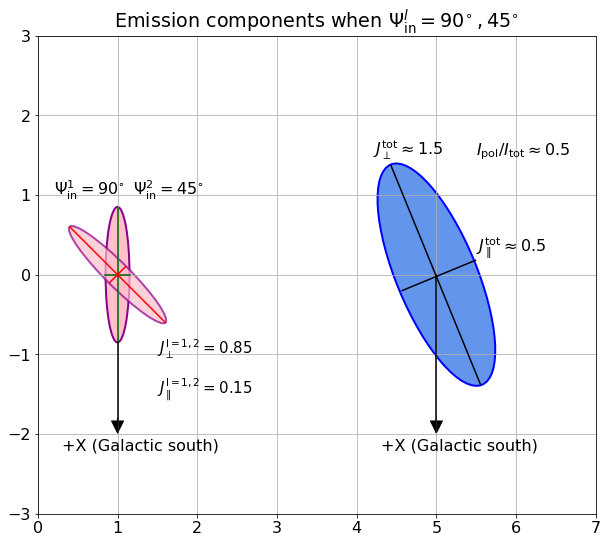
\includegraphics[width = 0.49\linewidth]{Images/Pol_intensity_Ellipses_circles_emissions.png}
%         \caption{Case II - Polarised intensity}
%         \label{fig_pol_intensity}
%     \end{subfigure}
%     \hfill
\caption{Simplified diagram of emission components for total and polarised intensities in terms of the polarisation ellipses.}
\end{figure*}

%\newpage

\section{Turbulent Magnetic Field}
\label{Appendix_B}
As discussed in section ~\ref{GMF} we generate the turbulent fields for our model using CRPropa3 ~\cite{CRPropa3_2016}. We the minimum and maximum wavelength we use to generate these fields are 
$L_{min}$ = 200 pc and $L_{max}$ = 400 pc and $L_{coh} \approx $~150 kpc. For all the three directions x,y and z we go from 1~pc to $\rm 8\times 10^{4}$~pc. One of the major reasons why we do not have enough decades covered for the wavelength is because of the time it takes to generate these fields using CRPropa. 
We looked at power spectrum for different realisations of the turbulent field. In figure ~\ref{fig:PowerSpectrum} we plot power spectrum in X,Y and Z directions by averaging over the other two directions. We chose this particular realisation since it followed closely a power law spectrum of index (5/3). 
\begin{figure}[h!]
    \centering
    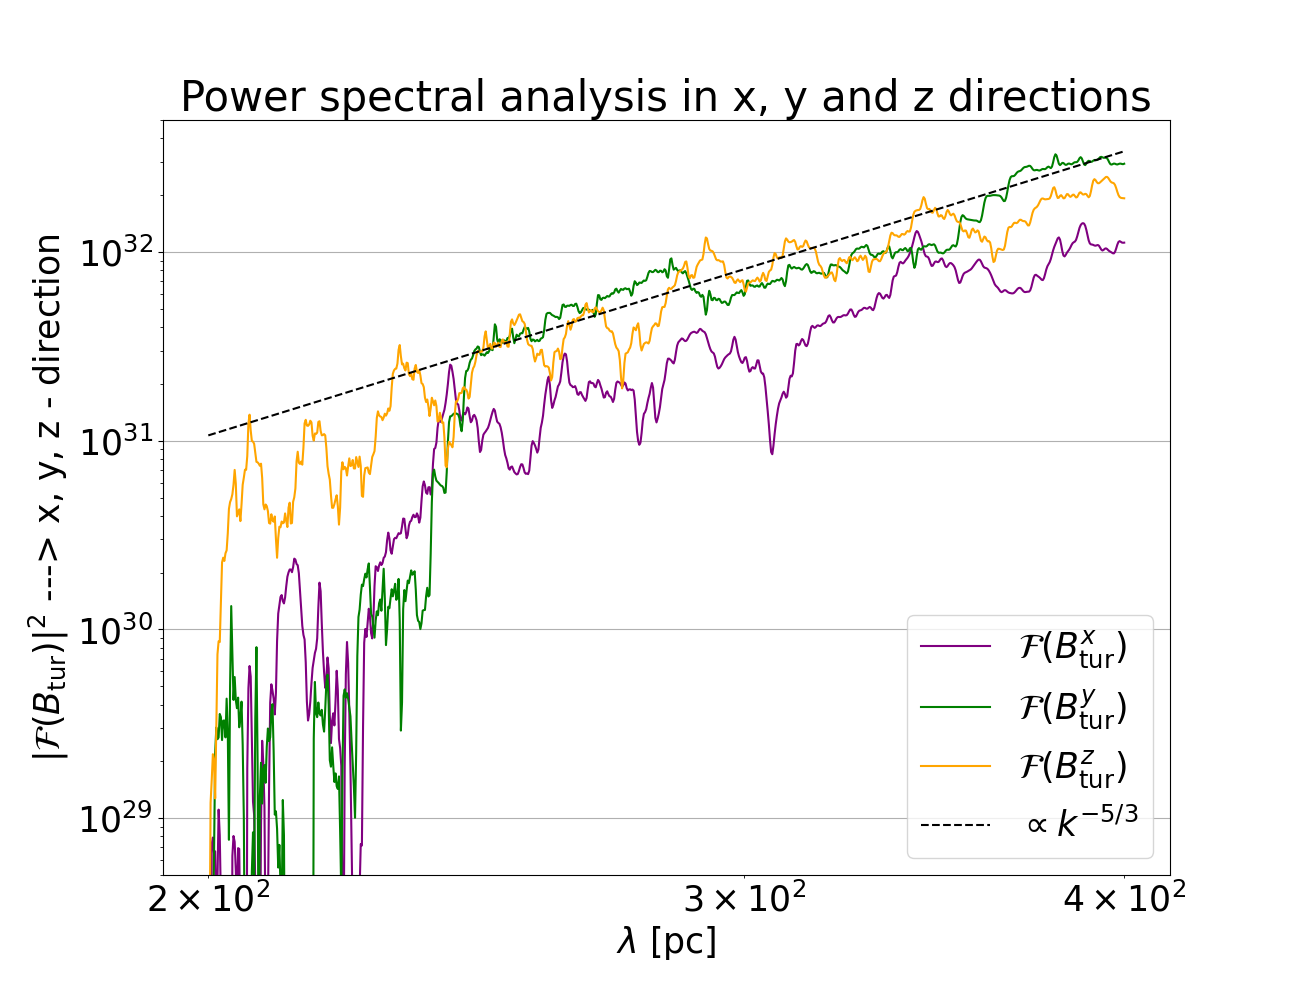
\includegraphics[width = 10cm]{Images/Jan27_Test_PowerSpectrum_vs_lambda_seed_10_lmin_200.0lmax_400.0.png}
    \caption{Power spectrum plot versus wavelength for X, Y and Z direction}
    \label{fig:PowerSpectrum}
\end{figure}

\iffalse

\newgeometry{top=20mm, bottom=20mm,lmargin=1.mm,rmargin=1.mm} 
\begin{figure}[h!]
    \centering
    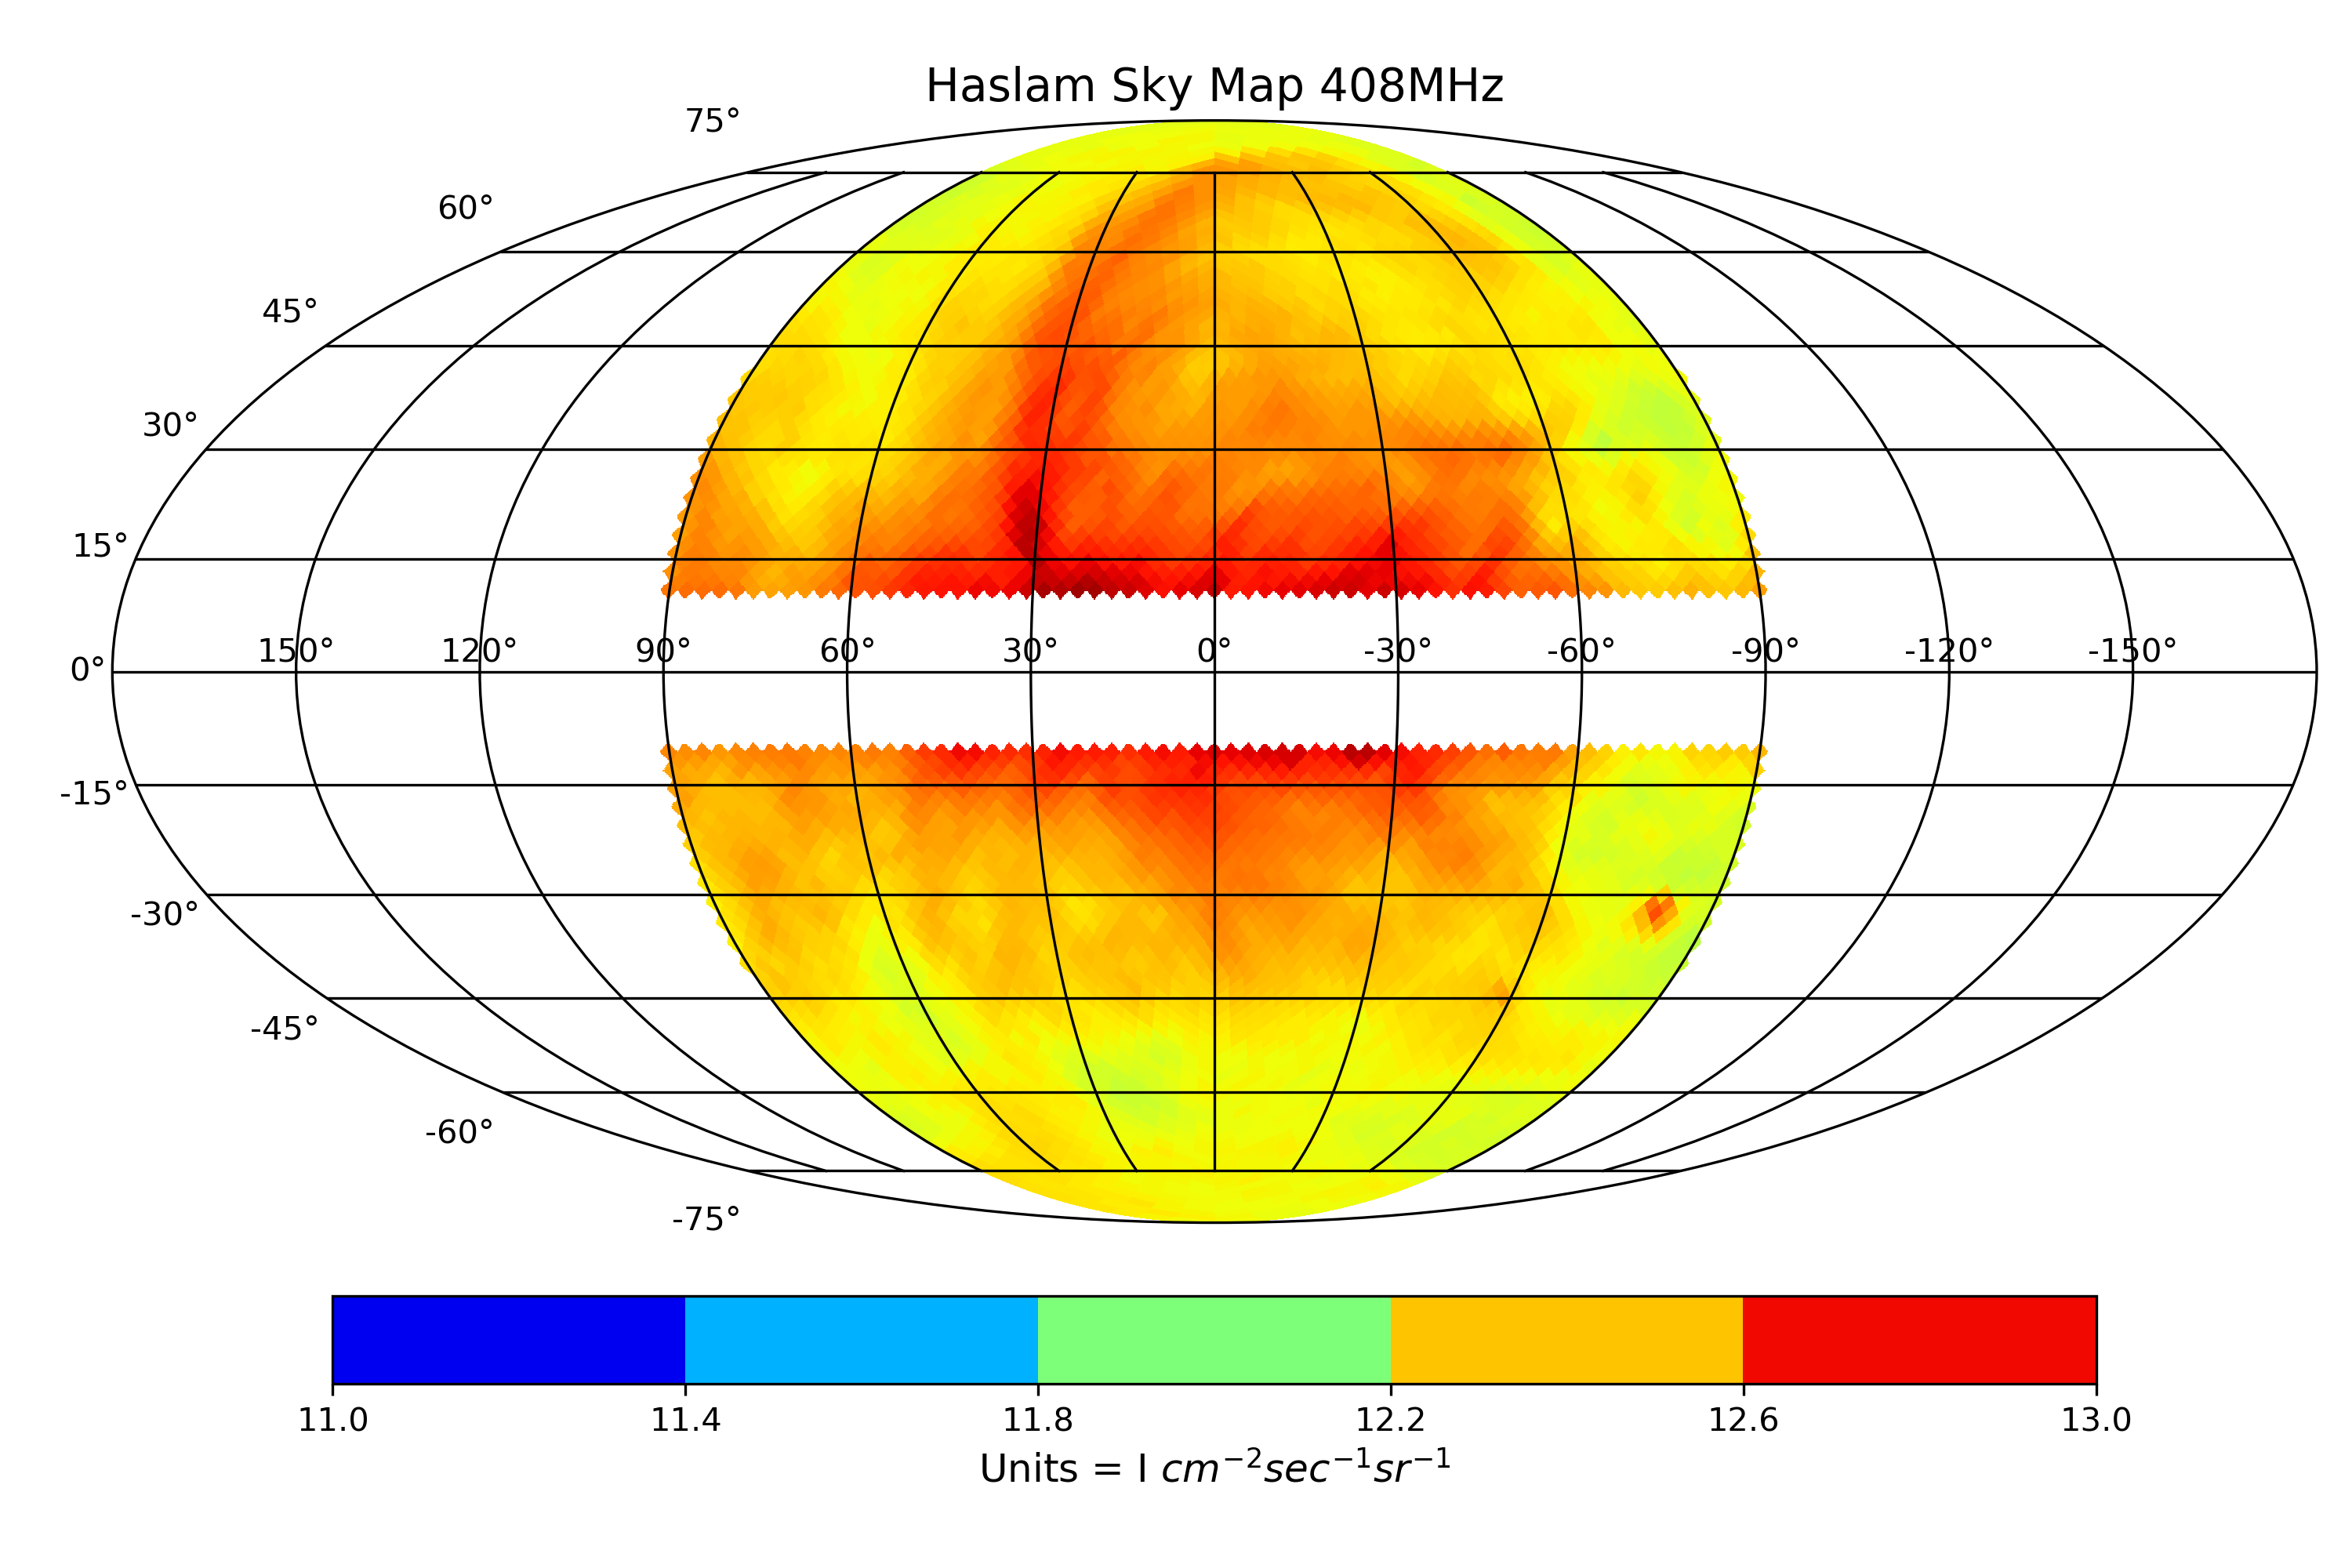
\includegraphics[width = 10cm]{Images/Haslam_408MHz.png}
    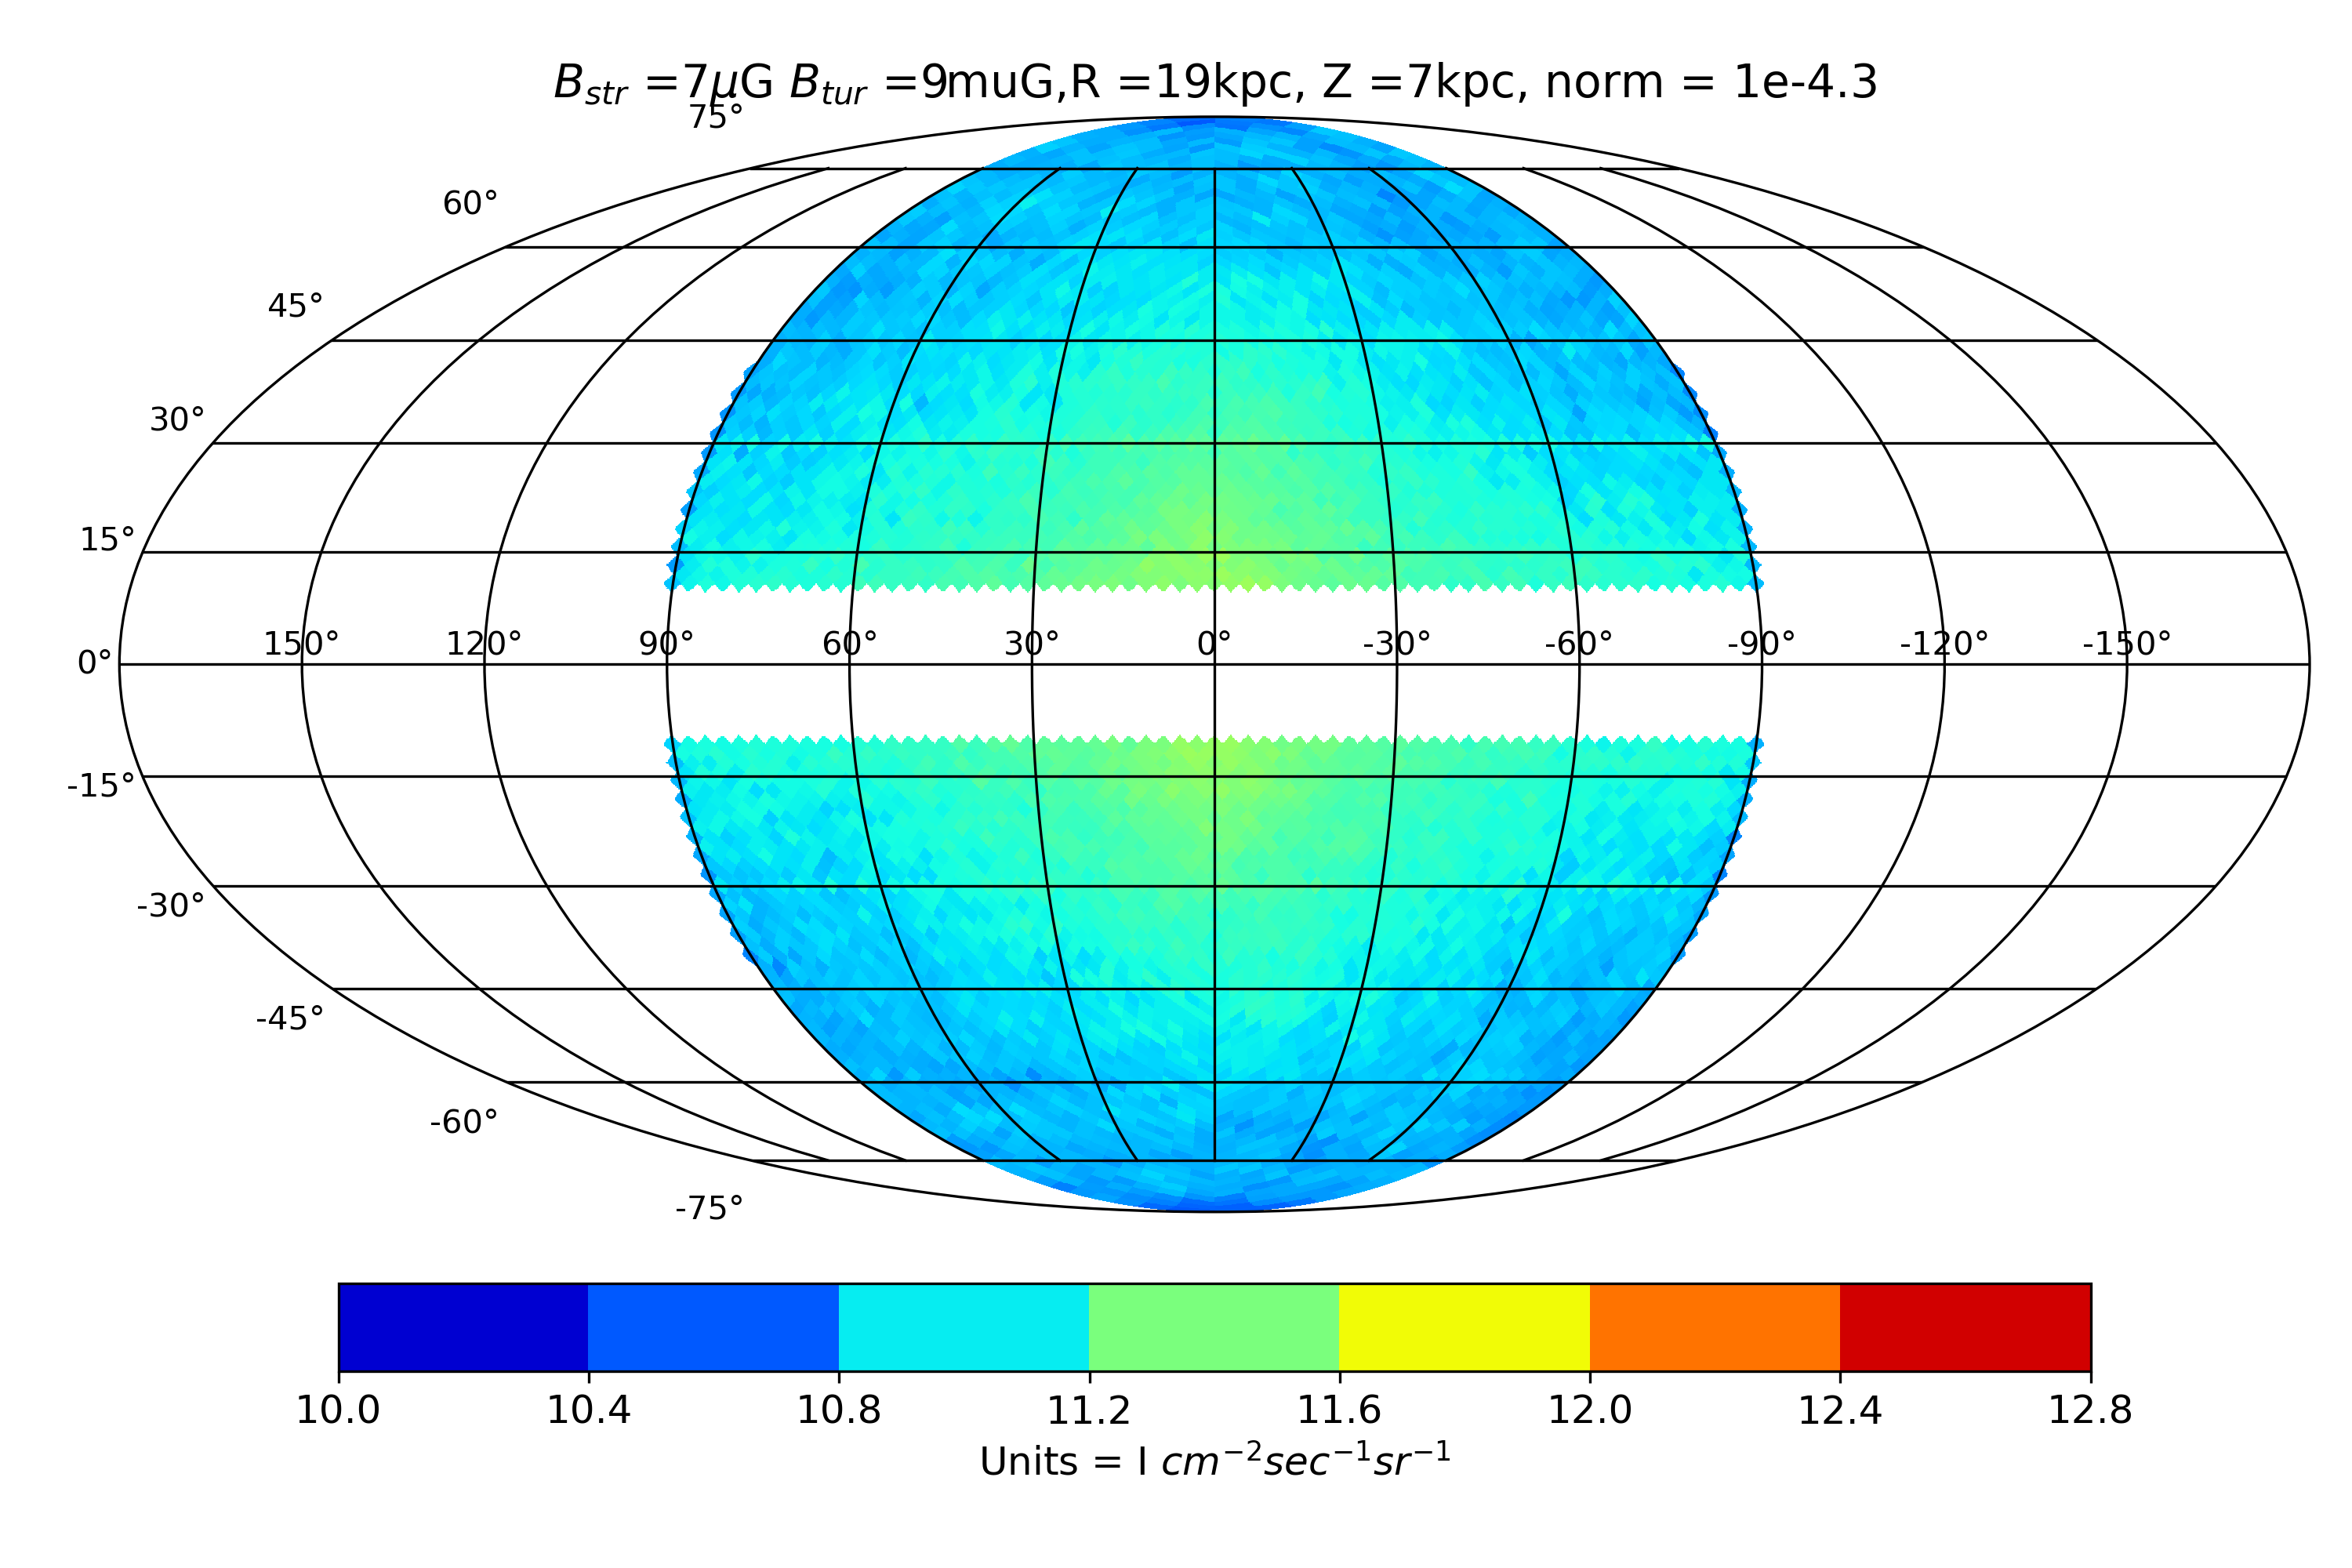
\includegraphics[width =
    10cm]{Images/408MHz_TI_Spec_Ind_3.0_Bstr_7_Btur_9_R_19_Z_7_norm_4.3.png}
 %   \includegraphics[width = 10cm]{Images/408MHz_TI_Spec_Ind_3.3_Bstr_5_Btur_10_R_12_Z_7.png}
    \caption{In figure Haslam data is shown top left, toy model total intensity map top right and in the bottom JF12 skymaps. The disc field is removed from this skymap and it includes Xfield, toroidal halo and turbulent fields.All calculated at $408$MHz. \Andrew{Color bar scales should have a fixed ranged (to allow easy comparison between maps)}}
    \label{fig:my_label}
\end{figure}
%\newpage

\fi


\end{document}
